\documentclass[11pt]{article}

\usepackage[a4paper, margin=1in]{geometry}
\usepackage{amsmath, amssymb}
\usepackage{graphicx}
\usepackage{booktabs}
\usepackage{caption}
\usepackage{subcaption}
\usepackage{float}
\usepackage{hyperref}
\usepackage{xcolor}
\usepackage{listings}

\title{Digital Image Processing --- Assignment 1}
\author{Ujjwal Gupta \\ Roll Number: 2024117015}
\date{\today}

\newcommand{\todoblock}[1]{\textcolor{red}{\textbf{TODO:} #1}}

\begin{document}

\maketitle

\section*{Machine specification}
All numbers reported below were measured on the following machine.

\begin{table}[H]
\centering
\begin{tabular}{ll}
\toprule
Item & Value \\
\midrule
CPU & Intel(R) Core(TM) i5-9300H CPU @ 2.40GHz (4 cores / 8 threads) \\
RAM & 14 GiB total \\
NumPy version & 2.5.2 \\
\bottomrule
\end{tabular}
\end{table}

\tableofcontents

%=======================================================================
\section{Problem 1 --- Convolution (30)}
%=======================================================================

\subsection{1.1 Correctness (6)}

Four implementations of 2-D convolution were built from scratch: \texttt{conv2d\_loops} (four
nested Python loops), \texttt{conv2d\_taps} (loop over the $k \times k$ kernel taps, vectorised
over the image), \texttt{conv2d\_im2col} (patch matrix followed by a single matrix--vector
product), and \texttt{conv2d\_fft} (multiplication in the frequency domain via
\texttt{numpy.fft}). All four use zero padding, \texttt{mode='same'}, and true convolution: the
kernel is flipped along both axes before the sliding sum (\texttt{K[::-1, ::-1]}), which is what
distinguishes convolution from correlation.

\paragraph{Verification against \texttt{scipy.signal.convolve2d}.} Tested on a $128 \times 128$
crop of \texttt{images/p1/base\_2048.png} with the $7\times7$ Gaussian kernel from the supplied
kernel bank, \texttt{mode='same'}, zero (\texttt{fill}) boundary.

\begin{table}[H]
\centering
\begin{tabular}{lc}
\toprule
Implementation & max $|$error$|$ vs \texttt{scipy.signal.convolve2d} \\
\midrule
\texttt{conv2d\_loops}  & $1.990\times10^{-13}$ \\
\texttt{conv2d\_taps}   & $1.990\times10^{-13}$ \\
\texttt{conv2d\_im2col} & $1.990\times10^{-13}$ \\
\texttt{conv2d\_fft}    & $2.274\times10^{-13}$ \\
\bottomrule
\end{tabular}
\caption{Maximum absolute error against the SciPy reference, $k=7$ Gaussian, $128\times128$ crop.}
\end{table}

All four agree with SciPy's reference to within floating-point round-off ($\sim 10^{-13}$), far
below the $1/255$ quantisation step of an 8-bit image, confirming correctness of all four
implementations. Figure~\ref{fig:error_heatmaps} shows the per-method $|\text{error}|$ map
against the SciPy reference --- uniformly at the $10^{-13}$ floor with no spatial structure, i.e.\
pure floating-point round-off rather than a systematic bug (a real bug, e.g.\ an unflipped kernel
or a padding off-by-one, would show up as a spatially structured error, typically concentrated at
the borders).

\begin{figure}[H]
\centering
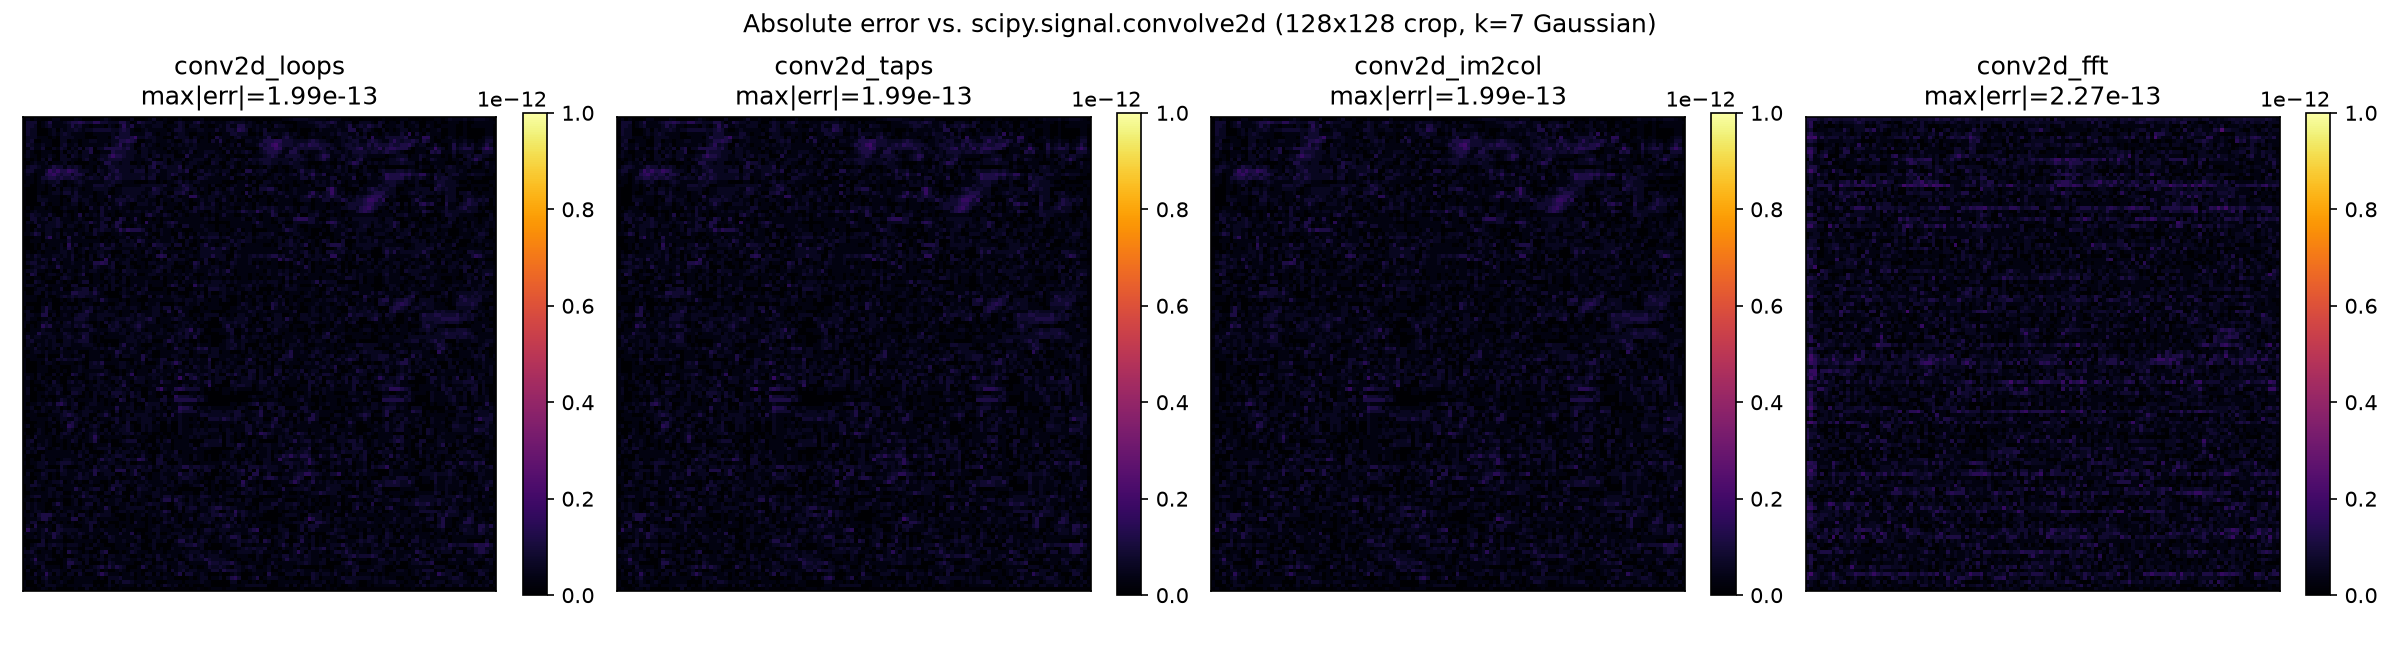
\includegraphics[width=\textwidth]{Images/p1_1_1_error_heatmaps.png}
\caption{Absolute error of each from-scratch implementation against the SciPy reference. All
four are flat at the $\sim10^{-13}$ floating-point floor with no spatial pattern.}
\label{fig:error_heatmaps}
\end{figure}

\paragraph{Asymmetric-kernel test: convolution vs.\ correlation.}
The \texttt{sobel3} kernel from the supplied bank,
\[
K = \begin{bmatrix} -1 & 0 & 1 \\ -2 & 0 & 2 \\ -1 & 0 & 1 \end{bmatrix},
\]
is antisymmetric under a $180^\circ$ flip: $K[::-1,::-1] = -K$. Convolution flips the kernel
before sliding; correlation does not. So for this kernel the two operations must produce exactly
negated results, unlike for a symmetric kernel (e.g.\ the Gaussian above) where flipping is a
no-op and convolution and correlation coincide.

This was verified on a $256\times256$ textured crop of \texttt{images/p1/base\_2048.png} (chosen
for visible structure; the flat $128\times128$ correctness-table crop shows almost no edge
content). Figure~\ref{fig:conv_vs_corr} shows, left to right: the input crop, the convolution
output, the correlation output, and their difference. At the pixel with the largest disagreement,
$(246, 255)$, convolution gives $+1013.0$ while correlation gives $-1013.0$ --- an exact sign
flip, as predicted, and visible in the figure as the convolution and correlation panels being
mirror images of each other in sign (blue and red swap) while sharing the same edge structure.

\begin{figure}[H]
\centering
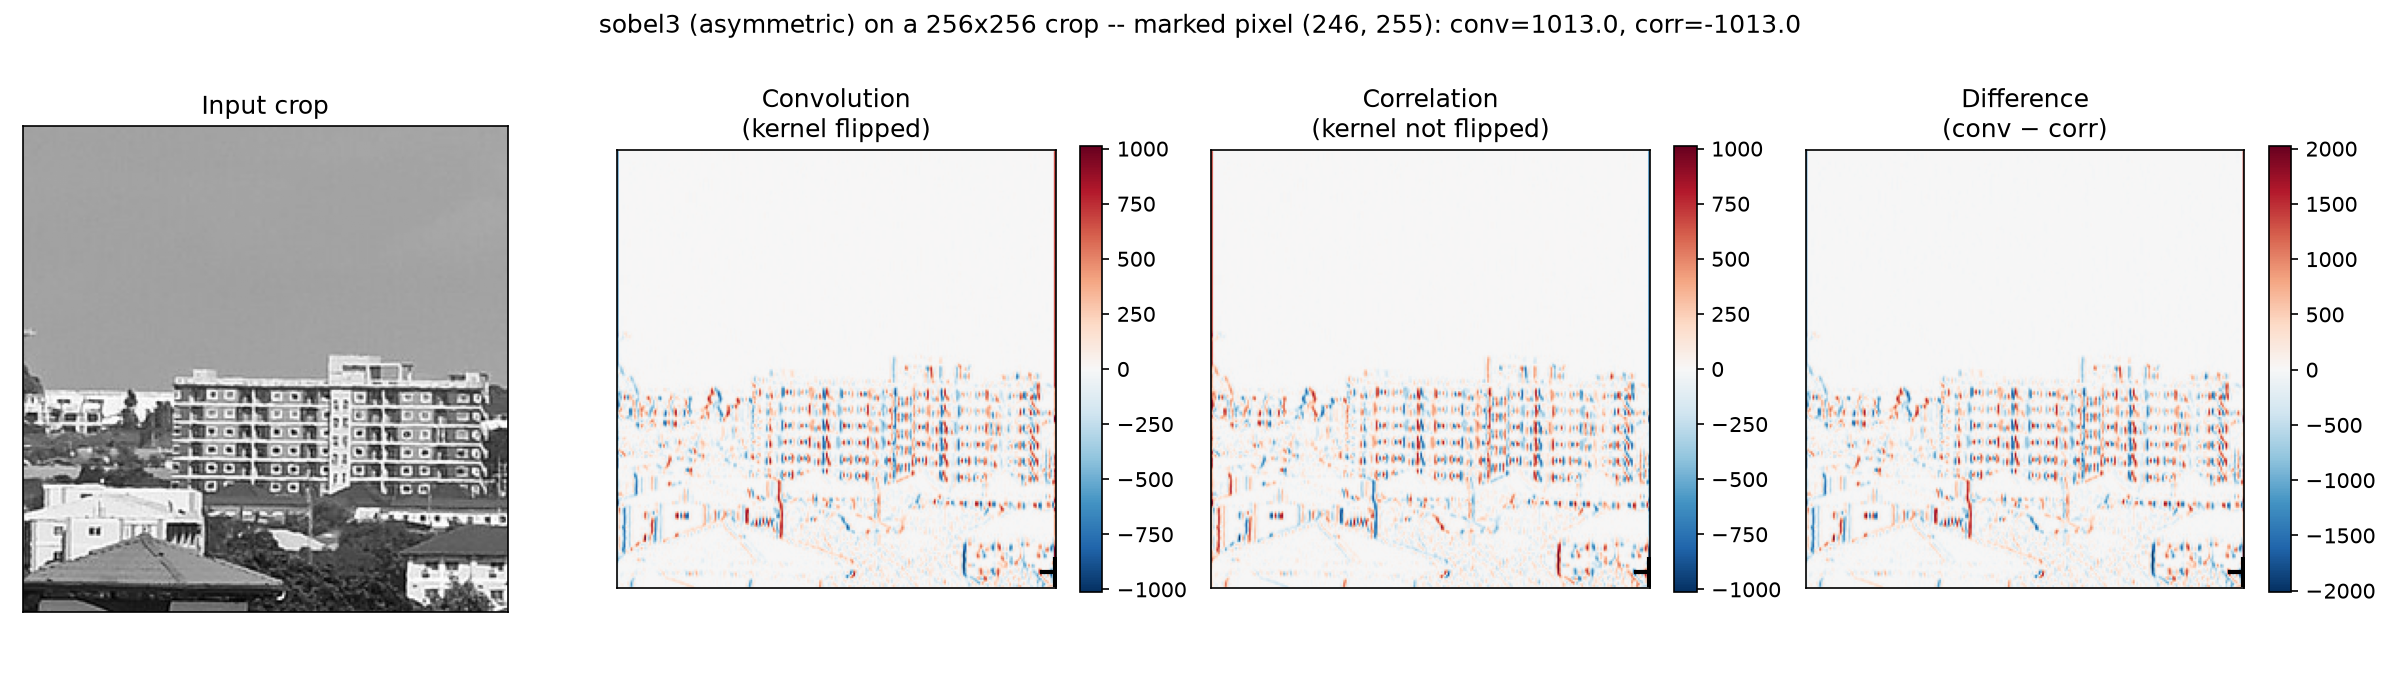
\includegraphics[width=\textwidth]{Images/p1_1_1_conv_vs_corr_sobel3.png}
\caption{Convolution vs.\ correlation with the asymmetric \texttt{sobel3} kernel on a
$256\times256$ crop of \texttt{base\_2048.png}. Convolution and correlation locate the same
edges but with opposite sign at every pixel, because flipping this antisymmetric kernel negates
it entirely ($K[::-1,::-1]=-K$); the marked pixel is where the two outputs disagree most.}
\label{fig:conv_vs_corr}
\end{figure}

\paragraph{Timing \texttt{conv2d\_loops} and extrapolating to full size.}
\texttt{conv2d\_loops} was timed on the $128\times128$ crop at $k=7$ (best of 3 runs), giving
$t_{128,7} = 0.375$\,s. The four nested Python loops make the cost scale as $O(HWk^2)$: linearly
in the number of output pixels $H \times W$ and quadratically in the kernel side $k$. This scaling
was checked empirically before extrapolating:

\begin{table}[H]
\centering
\begin{tabular}{lcc}
\toprule
Change & Measured ratio & Predicted ratio ($HWk^2$) \\
\midrule
$128\times128 \to 256\times256$ crop, $k=7$ fixed & $3.85\times$ & $4\times$ \\
$k{=}7 \to k{=}15$, $128\times128$ fixed & $4.46\times$ & $4.59\times$ \\
\bottomrule
\end{tabular}
\caption{Empirical scaling checks for \texttt{conv2d\_loops}, confirming $O(HWk^2)$ before
extrapolating to a size that was never actually run.}
\end{table}

Both measured ratios track the $O(HWk^2)$ prediction closely (small deviations are Python-loop
overhead noise, not a different asymptotic scaling). Extrapolating from $t_{128,7}$ to
$N=2048$, $k=15$:
\[
t_{2048,15} = t_{128,7} \times \underbrace{\frac{2048^2}{128^2}}_{256} \times
\underbrace{\frac{15^2}{7^2}}_{4.59} \approx 0.375 \times 256 \times 4.59 \approx 441\text{ s}
\;\;(\approx 7.3\text{ minutes}).
\]

This is why the handout does not ask for the full-size run: at $\sim 7$ minutes for a single
convolution, running \texttt{conv2d\_loops} at $2048\times2048, k{=}15$ would be a poor use of
time for a result already predictable from the loop structure. This cost motivates the vectorised
(\texttt{conv2d\_taps}), im2col, and FFT implementations benchmarked in
Section~\ref{sec:1.4}.

\subsection{1.2 Kernel rank (6)}

\paragraph{Threshold for calling a singular value zero.}
$\sigma_i$ is treated as zero if $\sigma_i \le \tau$, with
\[
\tau = \max(k_h, k_w) \cdot \sigma_{\max} \cdot \varepsilon_{\text{machine}},
\qquad \varepsilon_{\text{machine}} \approx 2.22\times10^{-16}\ \text{(float64)},
\]
matching \texttt{numpy.linalg.matrix\_rank}'s convention. Two properties motivate this choice
over a fixed absolute tolerance: (i) $\tau \propto \sigma_{\max}$ makes the reported rank
invariant to uniformly rescaling $K$ (rank is a shape property, not a normalisation), and (ii)
$\tau \propto \max(k_h,k_w)$ accounts for SVD round-off growing with matrix size. A fixed
absolute tolerance (e.g.\ $10^{-10}$) has neither property and can misclassify kernels that are
scaled very small or very large.

\paragraph{Rank table, $k=15$.}
\begin{table}[H]
\centering
% Auto-generated by run_1_2_rank.py -- do not edit by hand
\begin{tabular}{lccc}
\toprule
Kernel & Numerical rank & $\sigma_{\max}$ & threshold $\tau$ \\
\midrule
\texttt{box} & 1 & 6.667e-02 & 2.220e-16 \\
\texttt{gaussian} & 1 & 1.134e-01 & 3.777e-16 \\
\texttt{sobel3} & 1 & 3.464e+00 & 2.308e-15 \\
\texttt{log} & 2 & 9.680e-01 & 3.224e-15 \\
\texttt{log\_dc\_removed} & 3 & 9.638e-01 & 3.210e-15 \\
\texttt{motion\_0deg} & 1 & 2.582e-01 & 8.600e-16 \\
\texttt{motion\_45deg} & 15 & 6.667e-02 & 2.220e-16 \\
\texttt{disk} & 5 & 7.110e-02 & 2.368e-16 \\
\texttt{random} & 15 & 4.124e-02 & 1.374e-16 \\
\bottomrule
\end{tabular}

\caption{Numerical rank of every supplied kernel at $k=15$, with $\sigma_{\max}$ and the
threshold $\tau$ used to call a singular value zero.}
\label{tab:rank_table}
\end{table}

\begin{figure}[H]
\centering
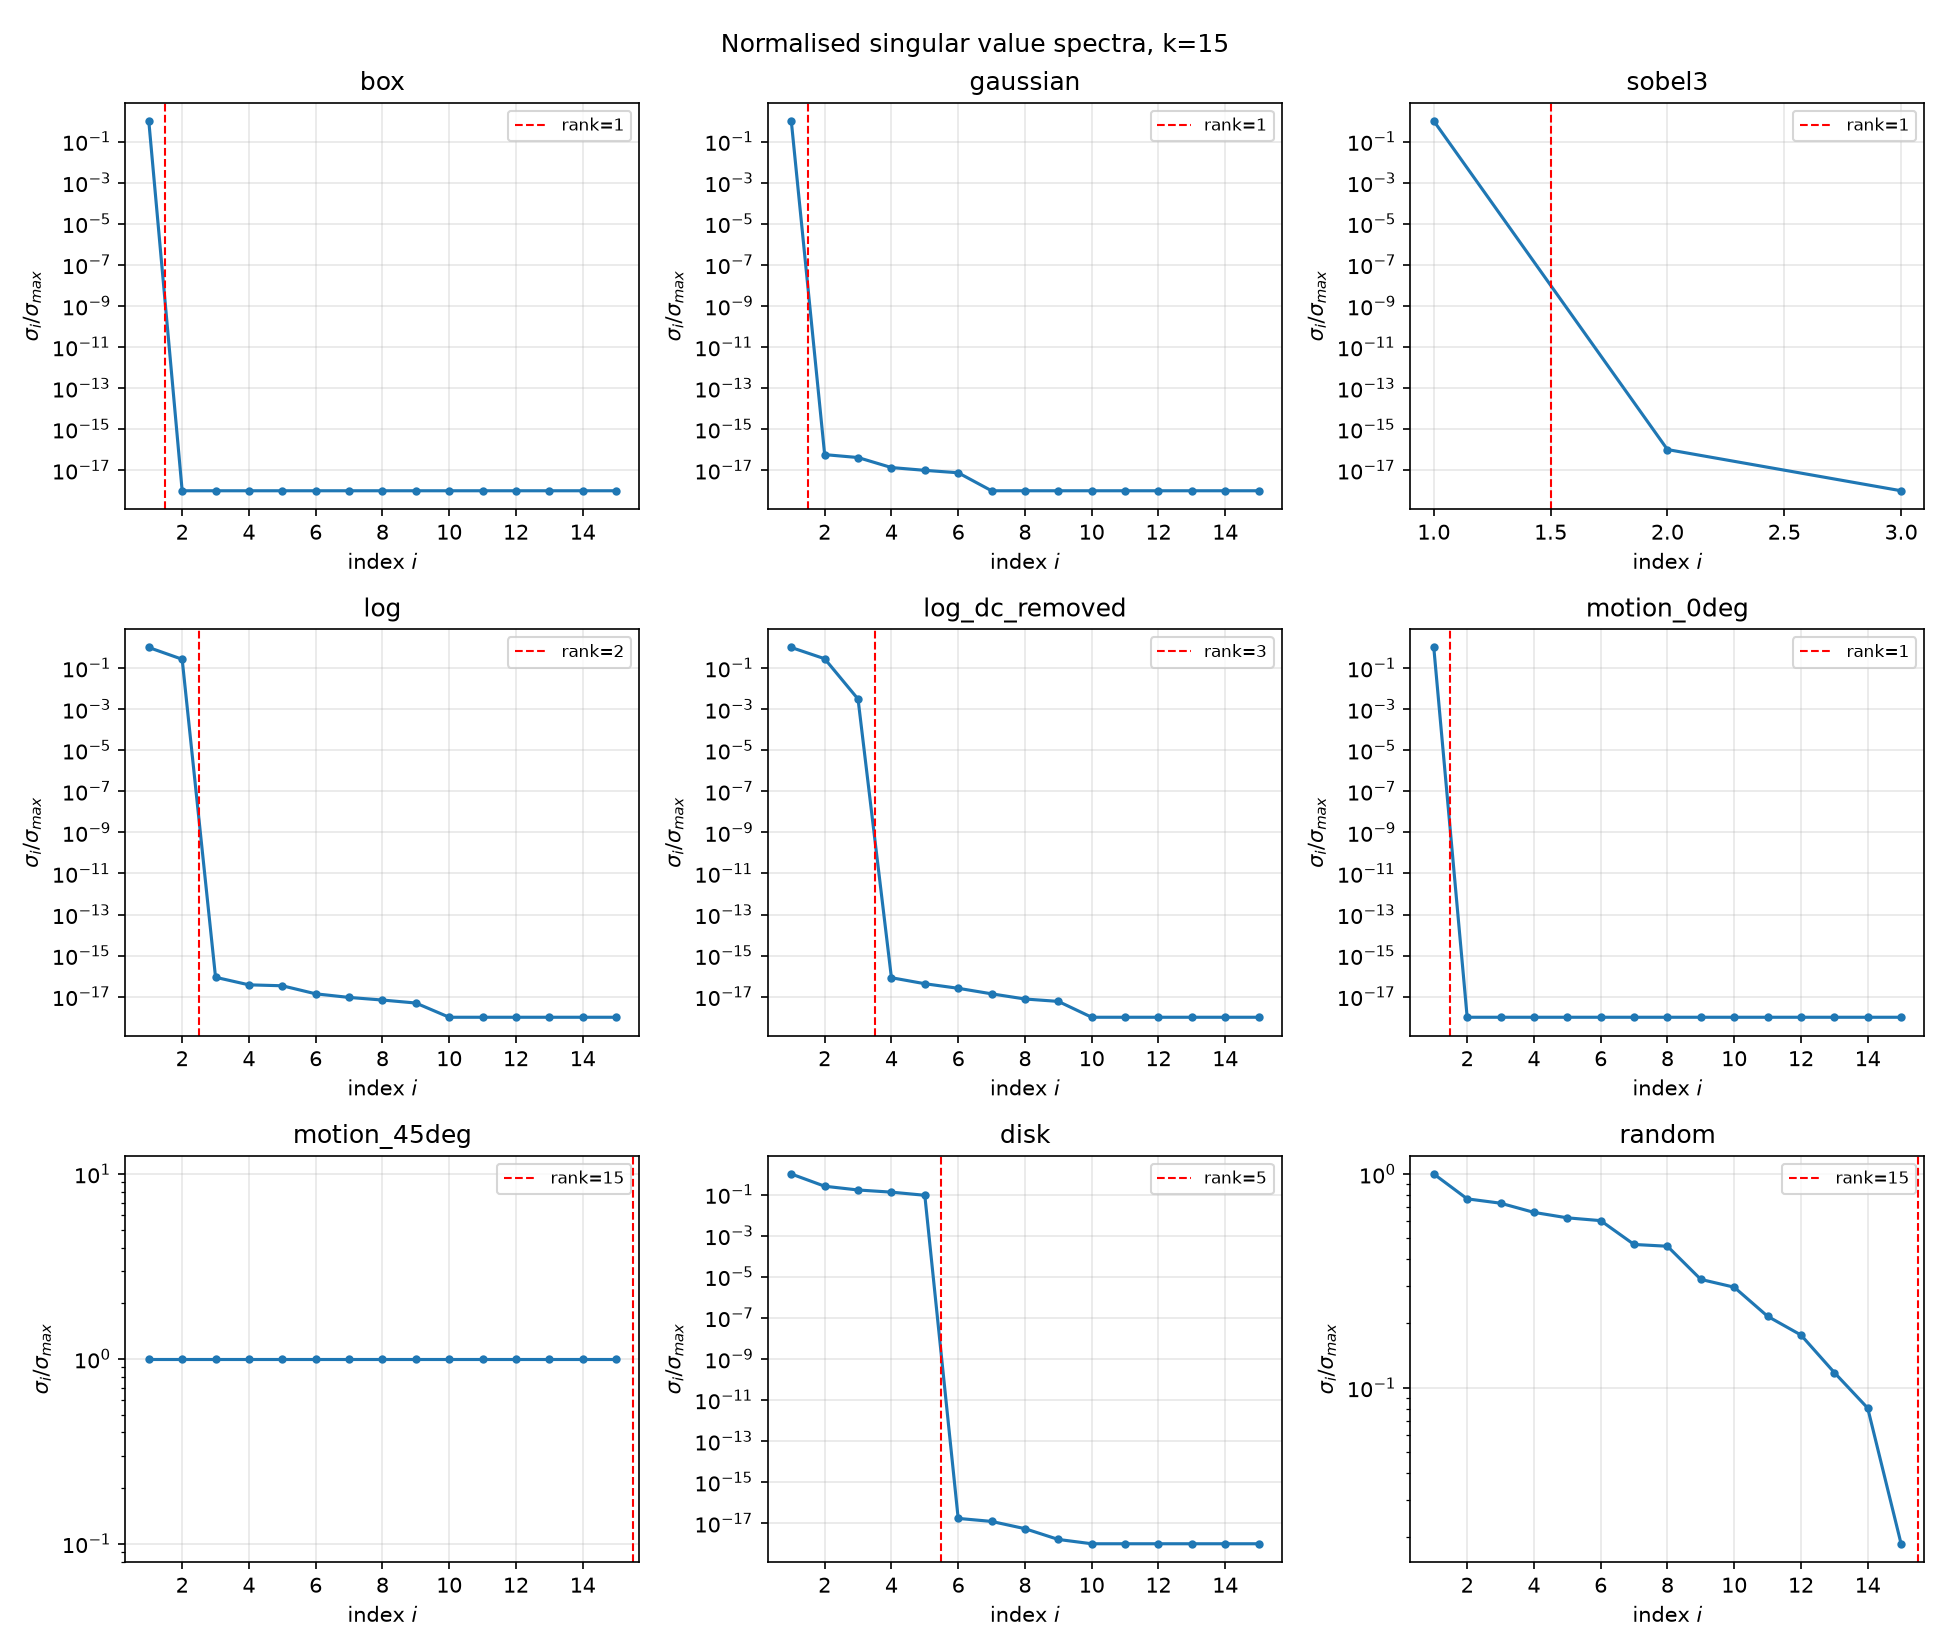
\includegraphics[width=\textwidth]{Images/p1_1_2_singular_spectra.png}
\caption{Normalised singular value spectra ($\sigma_i/\sigma_{\max}$, log scale), $k=15$. Red
dashed line marks the numerical rank; the spectrum drops to the $10^{-16}$--$10^{-17}$
floating-point floor immediately after it, except for \texttt{motion\_45deg} and
\texttt{random}, which decay smoothly (full rank).}
\label{fig:singular_spectra}
\end{figure}

\paragraph{(a) The raw LoG is exactly rank 2.}
\[
\text{LoG}(x,y) = -\frac{1}{\pi\sigma^4}\left(1 - \frac{x^2+y^2}{2\sigma^2}\right)
e^{-\frac{x^2+y^2}{2\sigma^2}}.
\]
With $g(x) = e^{-x^2/2\sigma^2}$ and $e^{-(x^2+y^2)/2\sigma^2} = g(x)g(y)$:
\[
\text{LoG}(x,y) \;\propto\; \left(1 - \frac{x^2}{2\sigma^2} - \frac{y^2}{2\sigma^2}\right) g(x)g(y)
= \underbrace{\left(1-\frac{x^2}{2\sigma^2}\right)g(x)}_{u_1(x)}\,\underbrace{g(y)}_{v_1(y)}
\;+\; \underbrace{g(x)}_{u_2(x)}\,\underbrace{\left(-\frac{y^2}{2\sigma^2}\right)g(y)}_{v_2(y)}.
\]
Sum of two rank-1 terms $\Rightarrow \text{rank} \le 2$. Not lower: $u_1$ (Gaussian $\times$
downward parabola, sign change at $x=\pm\sigma\sqrt2$) is not a scalar multiple of $u_2$ (pure
Gaussian, no sign change), so the two terms are linearly independent $\Rightarrow$ rank exactly
2, matching Table~\ref{tab:rank_table}.

\paragraph{(b) Mean subtraction raises LoG's rank from 2 to 3.}
Subtracting the mean $m$ adds $C = -m\cdot\mathbf{1}_{k\times k}$ (rank 1). Subadditivity gives
the upper bound
\[
\text{rank}(K_{\text{dc\_removed}}) = \text{rank}(K_{\text{raw}} + C) \le
\text{rank}(K_{\text{raw}}) + \text{rank}(C) = 2 + 1 = 3.
\]
This bound is not always tight: a rank-1 perturbation whose column space already lies inside the
original column space leaves the rank unchanged. Equality holds here because
$\mathbf{1}_k \notin \text{span}\{u_1, u_2\}$: $u_1, u_2$ are Gaussian-weighted and vanish near
the kernel edges, while $\mathbf{1}_k$ is constant to the border, so no combination of $u_1,u_2$
reproduces it. $\mathbf{1}_k$ is a genuinely new third direction $\Rightarrow$ rank exactly 3,
matching Table~\ref{tab:rank_table}.

\paragraph{(c) Motion blur at $0^\circ$ vs.\ $45^\circ$.}
\texttt{motion\_0deg} has one nonzero row ($1/k$ along the centre row); every other row is zero
$\Rightarrow$ rank 1 (it is the outer product $e_{k//2}\mathbf{1}_k^\top/k$, separable by
construction).

\texttt{motion\_45deg} $= I_k/k$ has its single nonzero entry in a different column for every
row, so no row is a multiple of another $\Rightarrow$ all $k$ rows independent $\Rightarrow$ full
rank $k=15$.

Both are physically the same operation (linear motion smear), but sampled rank depends on
alignment with the pixel grid. Axis-aligned smear stays within one row, which a rank-1 outer
product represents exactly. Diagonal smear advances one row \emph{and} one column per step, so no
single $(u,v)$ pair reproduces it via $uv^\top$: representing which column is active at each row
needs one degree of freedom per row, i.e.\ full rank. Separability is a property of how the
operator aligns with the sampling grid, not an invariant of the operator itself.

\subsection{1.3 Separability and low rank (10)}

\texttt{conv2d\_separable} uses the SVD $K = U S V^\top$, raises if $K$'s numeric rank exceeds 1,
and otherwise convolves with the flipped column factor $u_1[::-1]$ along one axis, then the
flipped row factor $v_1[::-1]$ along the other, scaled by $\sigma_1$: two $O(HWk)$ 1-D
convolutions instead of one $O(HWk^2)$ 2-D convolution. \texttt{conv2d\_lowrank} sums $r$ such
rank-1 passes from the truncated SVD, $K \approx \sum_{i=1}^r \sigma_i u_i v_i^\top$. Both were
checked against \texttt{conv2d\_fft}: \texttt{conv2d\_separable} matches to $\sim10^{-13}$ on the
rank-1 kernels \texttt{motion\_0deg} and \texttt{sobel3}, raises \texttt{ValueError} on the
rank-5 \texttt{disk} kernel, and \texttt{conv2d\_lowrank} at $r=k$ (full rank) recovers exact
convolution to $\sim10^{-13}$ for every kernel tested.

\paragraph{PSNR against $r$.}
Figure~\ref{fig:psnr_vs_r} plots PSNR of the rank-$r$ approximation against exact convolution
(\texttt{conv2d\_fft}) for \texttt{disk}, \texttt{log}, \texttt{motion\_45deg} and
\texttt{random} at $k=21$, on the top-left $512\times512$ crop of \texttt{base\_2048.png}.

\begin{figure}[H]
\centering
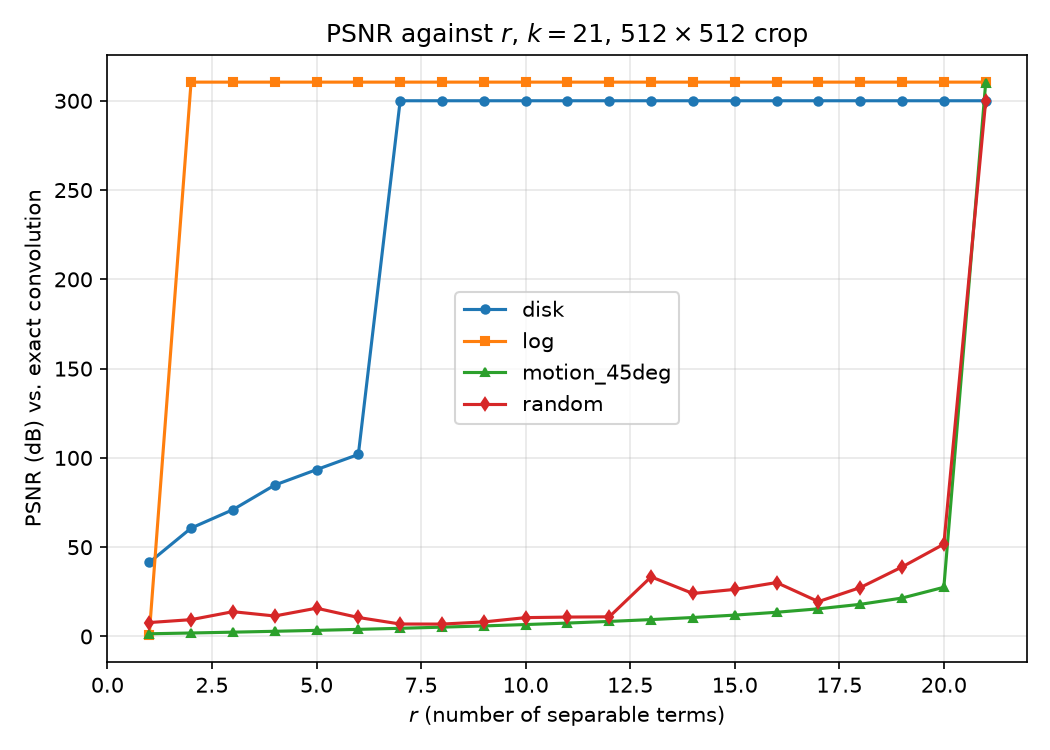
\includegraphics[width=0.75\textwidth]{Images/p1_1_3_psnr_vs_r.png}
\caption{PSNR of the rank-$r$ low-rank approximation vs.\ exact convolution, $k=21$,
$512\times512$ crop. \texttt{disk} and \texttt{log} reach near-exact fidelity within a handful
of terms; \texttt{motion\_45deg} and \texttt{random} stay poor until $r$ approaches $k$.}
\label{fig:psnr_vs_r}
\end{figure}

\texttt{log} reaches 310\,dB (numerically exact) by $r=3$, consistent with \S1.2's finding that
the raw LoG is exactly rank 2 (rank 2 also at $k=21$, by the same derivation --- see
Table~\ref{tab:energy_table}). \texttt{disk} reaches 71\,dB by $r=3$ and is exact by $r=10$.
\texttt{motion\_45deg} and \texttt{random} stay under 10\,dB until $r$ is nearly $k=21$, jumping
to $\sim300$\,dB only once $r$ reaches full rank.

\paragraph{Why disk needs few terms but motion-45\textdegree\ needs all $k$.}
Both are non-separable (rank $>1$), but PSNR at fixed $r$ depends on how the kernel's energy,
$\sum_i \sigma_i^2$, is distributed across singular values, not on rank alone. A rank-$r$
truncation captures the fraction of squared Frobenius norm $\sum_{i\le r}\sigma_i^2 \big/
\sum_i \sigma_i^2$; the closer this ratio is to 1 for small $r$, the smaller the approximation
error (dropped energy is the truncation's squared error, by the Eckart--Young theorem).

\begin{table}[H]
\centering
% Auto-generated by run_1_3_lowrank.py -- do not edit by hand
\begin{tabular}{lcccc}
\toprule
Kernel & rank & energy at $r{=}1$ & energy at $r{=}3$ & energy at $r{=}10$ \\
\midrule
\texttt{disk} & 7 & 89.23\% & 97.34\% & 100.00\% \\
\texttt{log} & 2 & 93.33\% & 100.00\% & 100.00\% \\
\texttt{motion\_45deg} & 21 & 4.76\% & 14.29\% & 47.62\% \\
\texttt{random} & 21 & 19.17\% & 41.27\% & 88.32\% \\
\bottomrule
\end{tabular}

\caption{Numerical rank and cumulative energy fraction $\sum_{i\le r}\sigma_i^2/\sum_i\sigma_i^2$
captured by the first $r$ singular values, $k=21$.}
\label{tab:energy_table}
\end{table}

\texttt{disk} is a smooth, roughly circularly-symmetric weighting; such kernels are well
approximated by a small number of separable (rank-1) "stripe" patterns, so its spectrum decays
fast --- 89\% of its energy is already in $\sigma_1$, 97\% by $\sigma_3$. \texttt{motion\_45deg}
$=I_k/k$ places equal weight $1/k$ on each of its $k$ singular values (a scaled identity is its
own SVD), so energy is spread \emph{uniformly}: capturing 47\% of it still needs 10 of 21 terms,
and no small truncation is good until $r$ is close to $k$. This is the general prediction rule:
\textbf{read the decay rate of the normalised singular value spectrum, not the rank}. A spectrum
that drops steeply after the first few terms (disk, log) is well approximated at small $r$
regardless of its exact rank; a flat or slowly-decaying spectrum (motion-45\textdegree, random)
needs $r$ close to the full rank for any accuracy, exactly as seen in
Figure~\ref{fig:spectra_linear} and predicted before ever running
\texttt{conv2d\_lowrank}.

\begin{figure}[H]
\centering
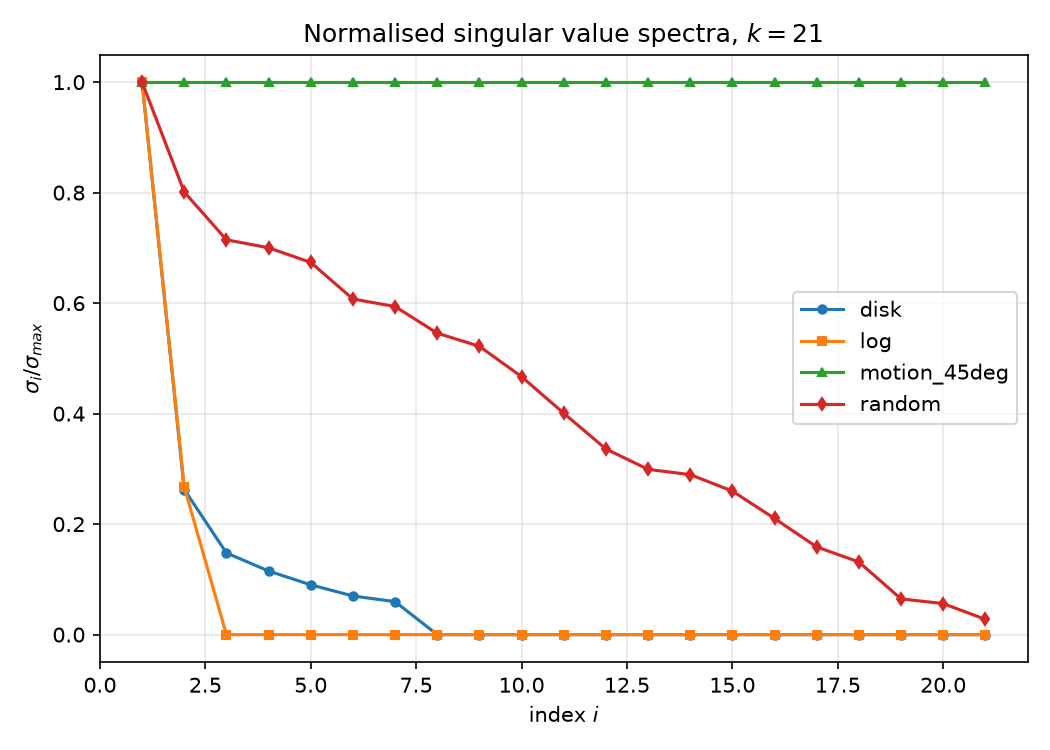
\includegraphics[width=0.75\textwidth]{Images/p1_1_3_spectra_linear.png}
\caption{Normalised singular value spectra (linear scale) for the four kernels in
Figure~\ref{fig:psnr_vs_r}. Steep early decay (disk, log) predicts good low-rank PSNR; flat
decay (motion-45\textdegree, random) predicts poor low-rank PSNR until $r \to k$.}
\label{fig:spectra_linear}
\end{figure}

\subsection{1.4 Runtime analysis (8)}
\label{sec:1.4}

All timings below use the separable Gaussian kernel (rank 1 at every $k$ tested, matching \S1.1)
and report the \emph{median} of 7 repetitions (3 for the two largest $N$, where each run already
takes seconds and repeated large allocations risk memory pressure --- see below). Median rather
than best-of-$N$ is used because best-of-$N$ at small $k$/$N$ is dominated by occasional fast
outlier runs from OS/GC scheduling noise, which distorts the fitted slope. \texttt{conv2d\_loops}
is excluded from both sweeps: \S1.1 measured $\sim$7 minutes for a single run at $N{=}2048,
k{=}15$, making a full sweep impractical.

\paragraph{Sweep 1: runtime vs.\ $k$, $N=512$.}
\begin{figure}[H]
\centering
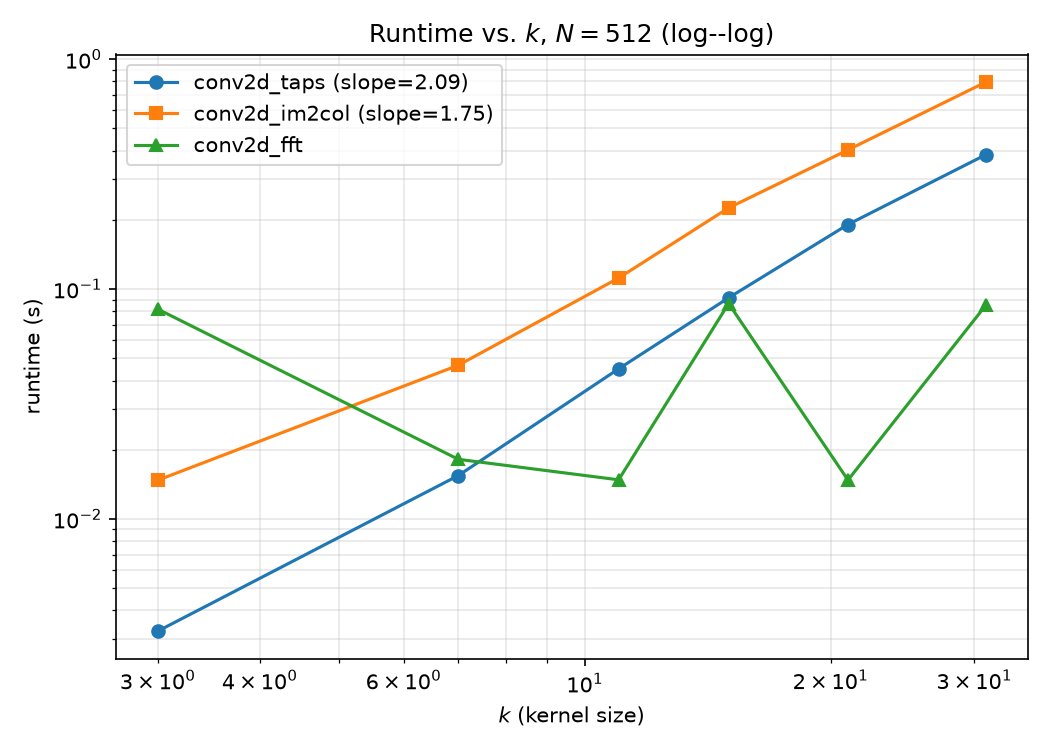
\includegraphics[width=0.75\textwidth]{Images/p1_1_4_runtime_vs_k.png}
\caption{Runtime vs.\ kernel size $k \in \{3,7,11,15,21,31\}$, $N=512$, log--log axes with
fitted power-law slopes.}
\label{fig:runtime_vs_k}
\end{figure}
Fitted slopes: \texttt{conv2d\_taps} $= 2.09$, \texttt{conv2d\_im2col} $=1.75$.
\texttt{conv2d\_fft}'s runtime is dominated by the fixed-size FFT of the $(N{+}k{-}1)$-padded
image rather than $k$, and does not follow a clean power law over this range.

\paragraph{Sweep 2: runtime vs.\ $N$, $k=15$.}
\begin{figure}[H]
\centering
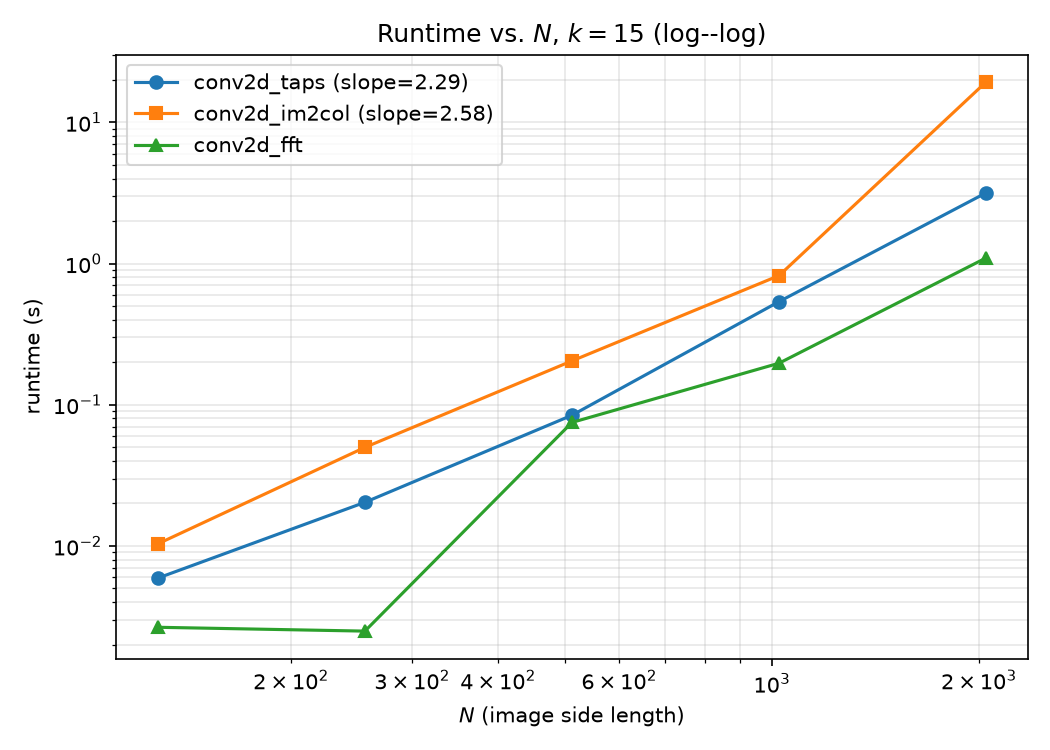
\includegraphics[width=0.75\textwidth]{Images/p1_1_4_runtime_vs_N.png}
\caption{Runtime vs.\ image side $N \in \{128,256,512,1024,2048\}$, $k=15$, log--log axes with
fitted power-law slopes.}
\label{fig:runtime_vs_N}
\end{figure}
Fitted slopes: \texttt{conv2d\_taps} $=2.29$, \texttt{conv2d\_im2col} $=2.58$ (inflated by the
memory-pressure effect at $N{=}2048$ discussed below); both are close to the $H W \propto N^2$
prediction.

\paragraph{Peak im2col memory.}
\texttt{conv2d\_im2col} materialises the patch matrix of shape $(HW,\ k_hk_w)$ in float64
(8 bytes/entry): $\text{bytes} = 8\,N^2 k^2$ for a square $N{\times}N$ image and $k{\times}k$
kernel. This is exactly $k^2$ times the size of the image itself, independent of $N$ (Table
\ref{tab:memory_table}, right column) --- every pixel's $k^2$-tap neighbourhood is copied out
in full, so the redundancy factor is fixed by the kernel footprint.

\begin{table}[H]
\centering
% Auto-generated by run_1_4_runtime.py -- do not edit by hand
\begin{tabular}{lccc}
\toprule
$N$ & patch matrix shape & peak memory (float64) & as fraction of image size \\
\midrule
128 & $(16384,\,225)$ & 29.5 MB & 225$\times$ \\
256 & $(65536,\,225)$ & 118.0 MB & 225$\times$ \\
512 & $(262144,\,225)$ & 471.9 MB & 225$\times$ \\
1024 & $(1048576,\,225)$ & 1887.4 MB & 225$\times$ \\
2048 & $(4194304,\,225)$ & 7549.7 MB & 225$\times$ \\
\bottomrule
\end{tabular}

\caption{Peak im2col patch-matrix memory at $k=15$ (225 taps/pixel), by image size.}
\label{tab:memory_table}
\end{table}

At $N=2048, k=15$ the patch matrix alone is 7.5\,GB, on a 14\,GiB-RAM machine already holding the
original image, padded copy, and Python/NumPy overhead. In this regime im2col's runtime became
unreliable across repeated runs: an early run measured 7.7\,s, a later run of the same
computation (with other memory already in use, confirmed via \texttt{free -h} showing $\sim$2.4\,GiB
of swap in use at the time) measured 19.3\,s for the same array shapes. The formula makes this
predictable: at $N{=}4096$ the same kernel would need $8\times4096^2\times225 \approx 30$\,GB,
exceeding this machine's RAM outright, so \texttt{conv2d\_im2col} would start swapping
continuously or fail to allocate --- the technique's cost is memory-bound at large $N$, not
compute-bound.

\paragraph{(a) Why the fitted tap-loop slope is not below 2.}
On this machine the measured slope vs.\ $k$ is $2.09$ --- at, not below, the theoretical $k^2$.
\texttt{conv2d\_taps} loops over $k^2$ taps in Python, but the $O(HW)$ work per tap is a single
vectorised NumPy slice-multiply-accumulate; there is no per-tap Python-level overhead that would
amortise away as $k$ grows, unlike loop-unrolling overhead in a hand-written low-level loop. Each
of the $k^2$ taps does a fixed, non-shrinking amount of work ($O(HW)$ memory reads and
multiply-adds), so this implementation has no mechanism to produce a sub-quadratic slope. A slope
below 2 would instead need per-tap Python overhead that amortises over more work as $k$ grows, or
SIMD/cache reuse that improves with wider taps --- neither applies to independent full-image
NumPy slice operations.

\paragraph{(b) Does im2col beat the tap loop here?}
No: at every $k$ and every $N$ tested, \texttt{conv2d\_im2col} is slower than
\texttt{conv2d\_taps} (Figures~\ref{fig:runtime_vs_k}--\ref{fig:runtime_vs_N}) --- roughly
2--3$\times$ slower across the range, and far worse at $N{=}2048$ under memory pressure. im2col
wins in deep-learning frameworks because those systems (a) run on GPUs, where the patch-matrix
construction and the matmul both map to massively parallel, highly optimised BLAS kernels, and
(b) reuse the same im2col'd input across many different kernels in a batch (many output
channels), amortising the one-time cost of building the patch matrix over many matmuls. Here,
each call reruns the patch extraction for a single kernel on a single CPU core via
\texttt{sliding\_window\_view} plus a materialising \texttt{reshape}, so the patch matrix's
construction cost is paid in full for a single convolution and never amortised: neither condition
that lets im2col win holds in this benchmark.

\paragraph{(c) Separable speedup at $512^2$ vs.\ $2048^2$.}
\begin{table}[H]
\centering
% Auto-generated by run_1_4_runtime.py -- do not edit by hand
\begin{tabular}{lccc}
\toprule
$N$ & \texttt{conv2d\_taps} & \texttt{conv2d\_separable} & measured speedup ($k/2=7.5\times$ theory) \\
\midrule
512 & 0.0810s & 0.0142s & 5.69$\times$ \\
2048 & 2.9398s & 0.4154s & 7.08$\times$ \\
\bottomrule
\end{tabular}

\caption{\texttt{conv2d\_separable} speedup over \texttt{conv2d\_taps} at $k=15$ (theoretical
$k/2=7.5\times$).}
\label{tab:speedup_table}
\end{table}
The measured speedup is $5.7\times$ at $512^2$ but $7.1\times$ at $2048^2$ --- closer to the
$7.5\times$ theoretical value at the larger size. At $512^2$ both the 2-D tap loop and the two
1-D passes finish in tens of milliseconds, where fixed per-call Python/NumPy overhead (function
calls, array allocation, padding) is a larger fraction of the total time and is not itself
$k$-dependent; this overhead is paid twice by the separable version (once per 1-D pass) but
included in the $2HWk$ separable cost either way, so it dilutes the achieved speedup below the
asymptotic $k/2$. At $2048^2$ the actual per-tap arithmetic dominates both implementations'
runtime, the fixed overhead becomes negligible by comparison, and the measured speedup converges
towards the asymptotic prediction.

%=======================================================================
\section{Problem 2 --- Bit-plane slicing and steganography (20)}
%=======================================================================

\subsection{2.1 Decomposition (5)}

\paragraph{Bit planes.} \texttt{cover\_textured.png} decomposed into its 8 bit planes via
$(\text{img} \gg b)\ \&\ 1$, $b=0$ (LSB) to $b=7$ (MSB).

\begin{figure}[H]
\centering
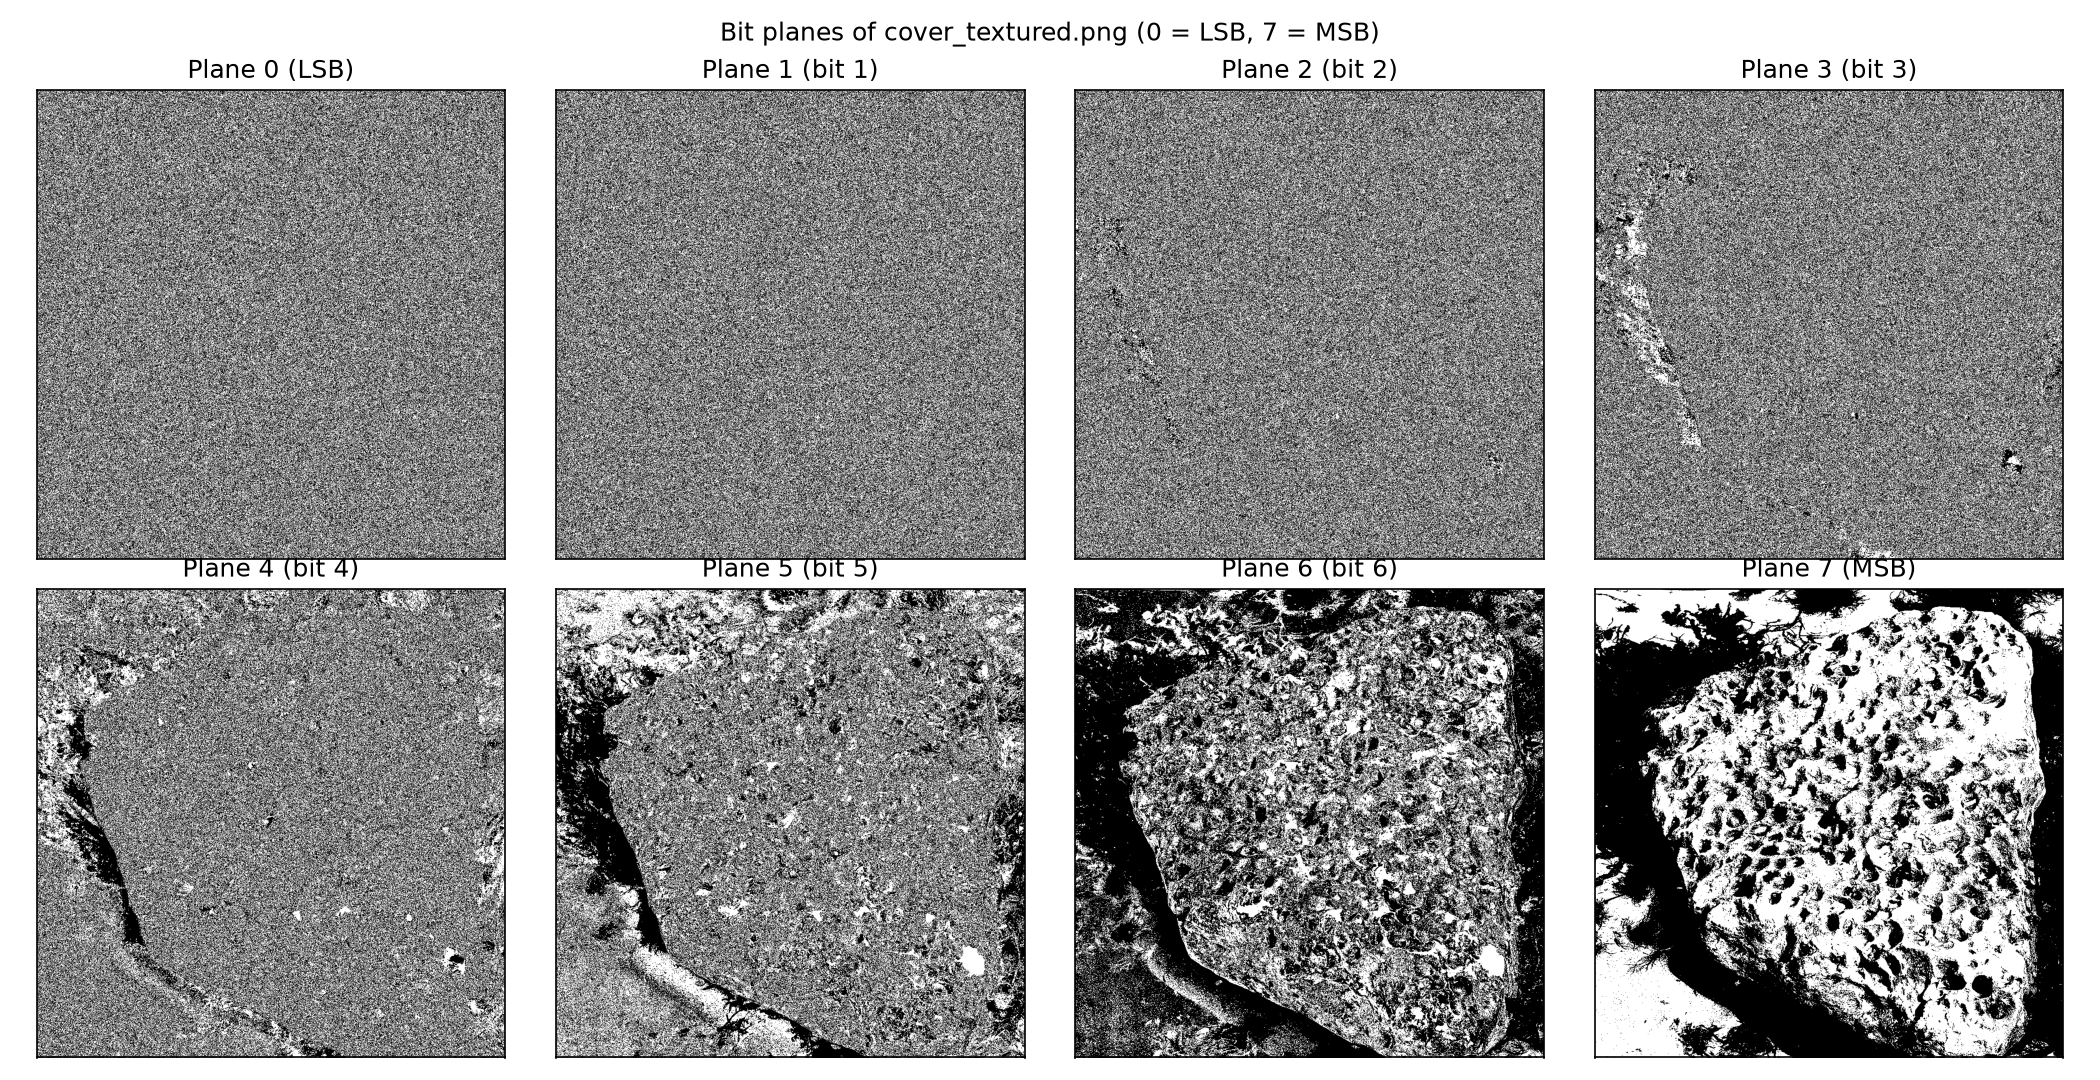
\includegraphics[width=\textwidth]{Images/p2_2_1_bit_planes.png}
\caption{Eight bit planes of \texttt{cover\_textured.png}. High planes (6, 7) carry recognisable
image structure; low planes (0--2) look like noise.}
\label{fig:bit_planes}
\end{figure}

\paragraph{PSNR against $n$.}
\begin{figure}[H]
\centering
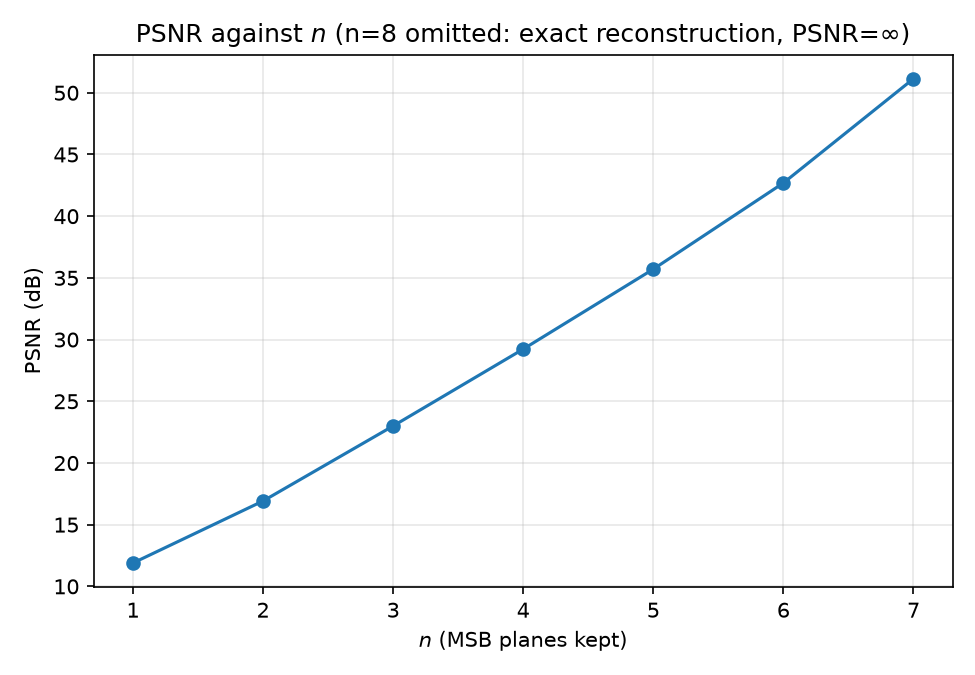
\includegraphics[width=0.65\textwidth]{Images/p2_2_1_psnr_vs_n.png}
\caption{PSNR of the reconstruction from the top $n$ MSB planes vs.\ the original ($n=8$ is
exact, PSNR$=\infty$, omitted from the axis).}
\label{fig:psnr_vs_n}
\end{figure}

\begin{table}[H]
\centering
\begin{tabular}{lccccccc}
\toprule
$n$ & 1 & 2 & 3 & 4 & 5 & 6 & 7 \\
\midrule
PSNR (dB) & 11.89 & 16.92 & 23.00 & 29.23 & 35.71 & 42.69 & 51.14 \\
\bottomrule
\end{tabular}
\caption{PSNR against $n$ MSB planes kept; mean per-plane gain $\approx 6.5$\,dB.}
\end{table}

Keeping only the top $n$ MSB planes is uniform quantisation with step size
$\Delta_n = 2^{8-n}$: one more plane halves the step, $\Delta_n = \Delta_{n-1}/2$. For a uniform
quantiser the reconstruction MSE is $\Delta^2/12$, so adding a plane reduces MSE by exactly
$4\times$, and
\[
\Delta\text{PSNR} = 10\log_{10}\!\left(\frac{\text{MSE}_{n-1}}{\text{MSE}_n}\right)
= 10\log_{10}(4) \approx 6.02\text{ dB},
\]
independent of image content --- this is the classical "6\,dB per bit" quantisation-noise rule.
The measured gain ($\approx6.5$\,dB, close to but slightly above 6.02) matches this prediction;
the small excess comes from \texttt{reconstruct} truncating to the kept planes (equivalent to
always rounding down within each quantisation bin) rather than rounding to bin centre, which
would shift MSE by a content-independent constant without changing the $4\times$ ratio between
successive $n$.

\paragraph{Ramp: binary vs.\ Gray code.}
\begin{figure}[H]
\centering
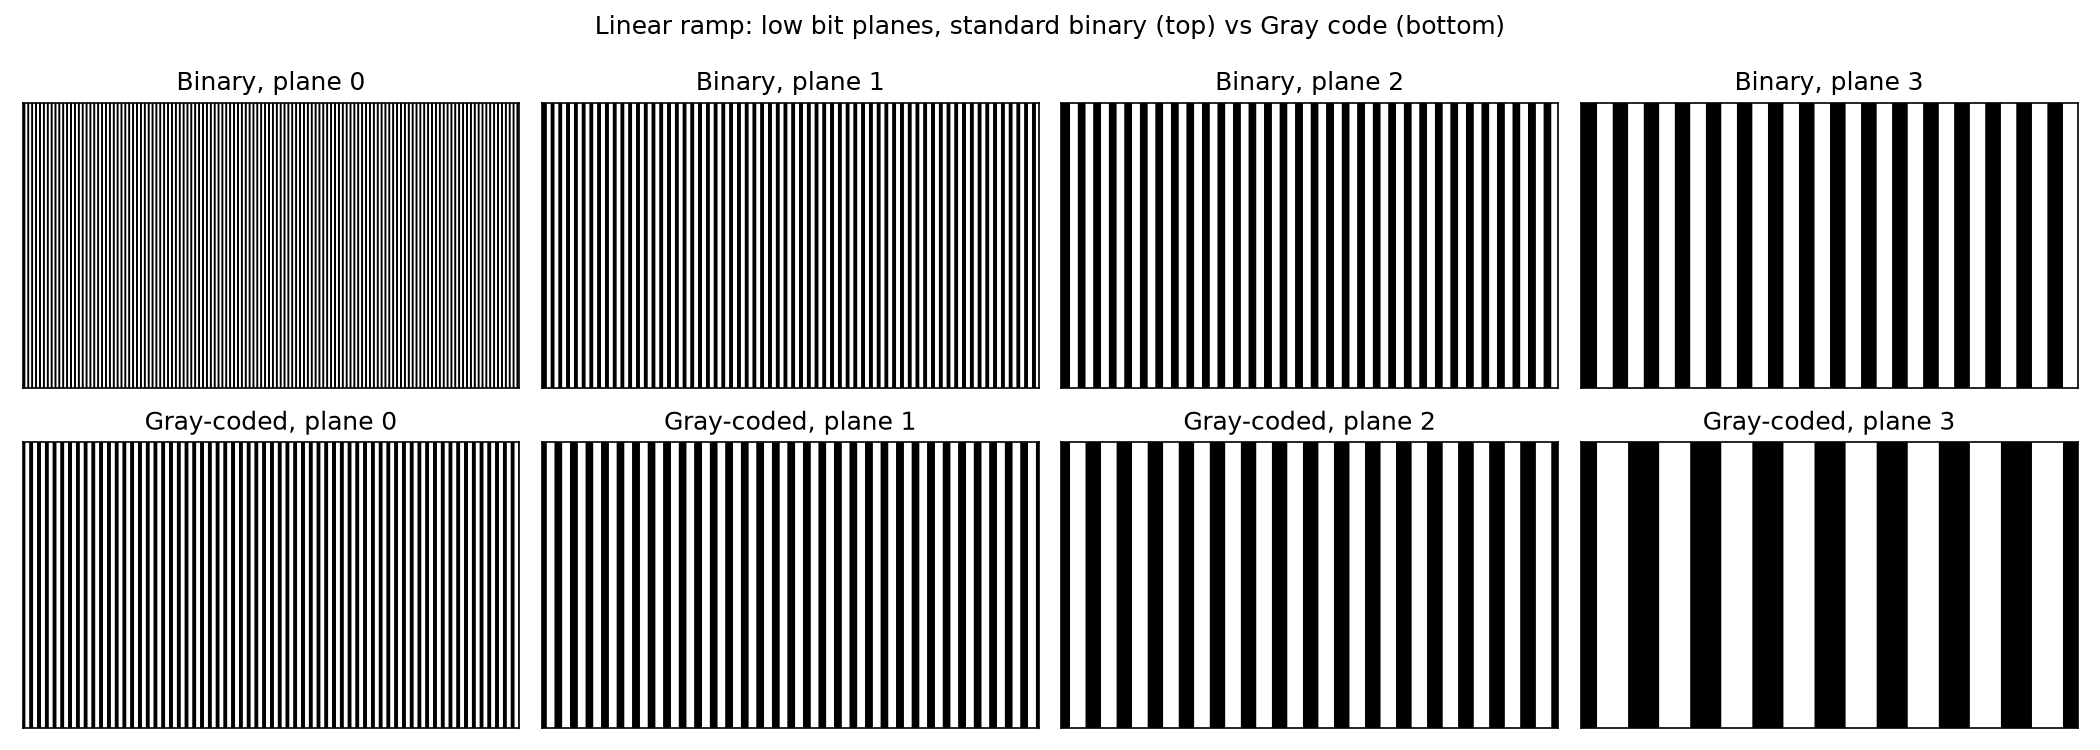
\includegraphics[width=\textwidth]{Images/p2_2_1_ramp_gray_comparison.png}
\caption{Low bit planes of a constructed linear ramp, standard binary encoding (top) vs.\
Gray-coded intensities (bottom).}
\label{fig:ramp_gray}
\end{figure}
The ramp's low planes under standard binary encoding show a regular, high-frequency
\emph{striped} pattern --- plane $b$ toggles every $2^b$ pixels along the ramp, a direct artefact
of binary counting (unlike a natural image, whose low planes look like unstructured noise because
neighbouring pixel values are not perfectly linearly increasing). This is the well-known
weakness of standard binary bit-plane encoding: a value change of just 1 grey level can flip
many bits at once (e.g.\ $127 \to 128$ flips all 8 bits), producing these visible stripes even
though the underlying signal is smooth. Gray coding (bottom row) guarantees adjacent intensities
differ in exactly one bit, so each plane instead shows broader, coarser bands rather than tight
periodic stripes, and no plane is disturbed by a carry propagating through multiple bit
positions.

\subsection{2.2 Hide and recover a payload (5)}

\paragraph{Recovery.} Reading plane-0 LSBs of \texttt{decode\_me.png} in raster order recovers
the sync marker \texttt{10101010} exactly, followed by height $=64$, width $=64$
(bits 8--23, MSB-first), and a $64\times64$ payload (bits 24 onward).

\begin{figure}[H]
\centering
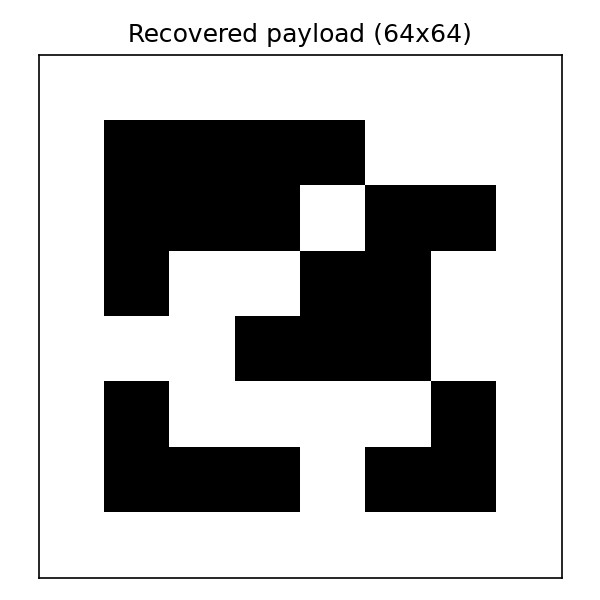
\includegraphics[width=0.35\textwidth]{Images/p2_2_2_recovered_payload.png}
\caption{Recovered $64\times64$ binary payload from \texttt{decode\_me.png}.}
\label{fig:recovered_payload}
\end{figure}

\paragraph{PSNR and visibility.}
\begin{figure}[H]
\centering
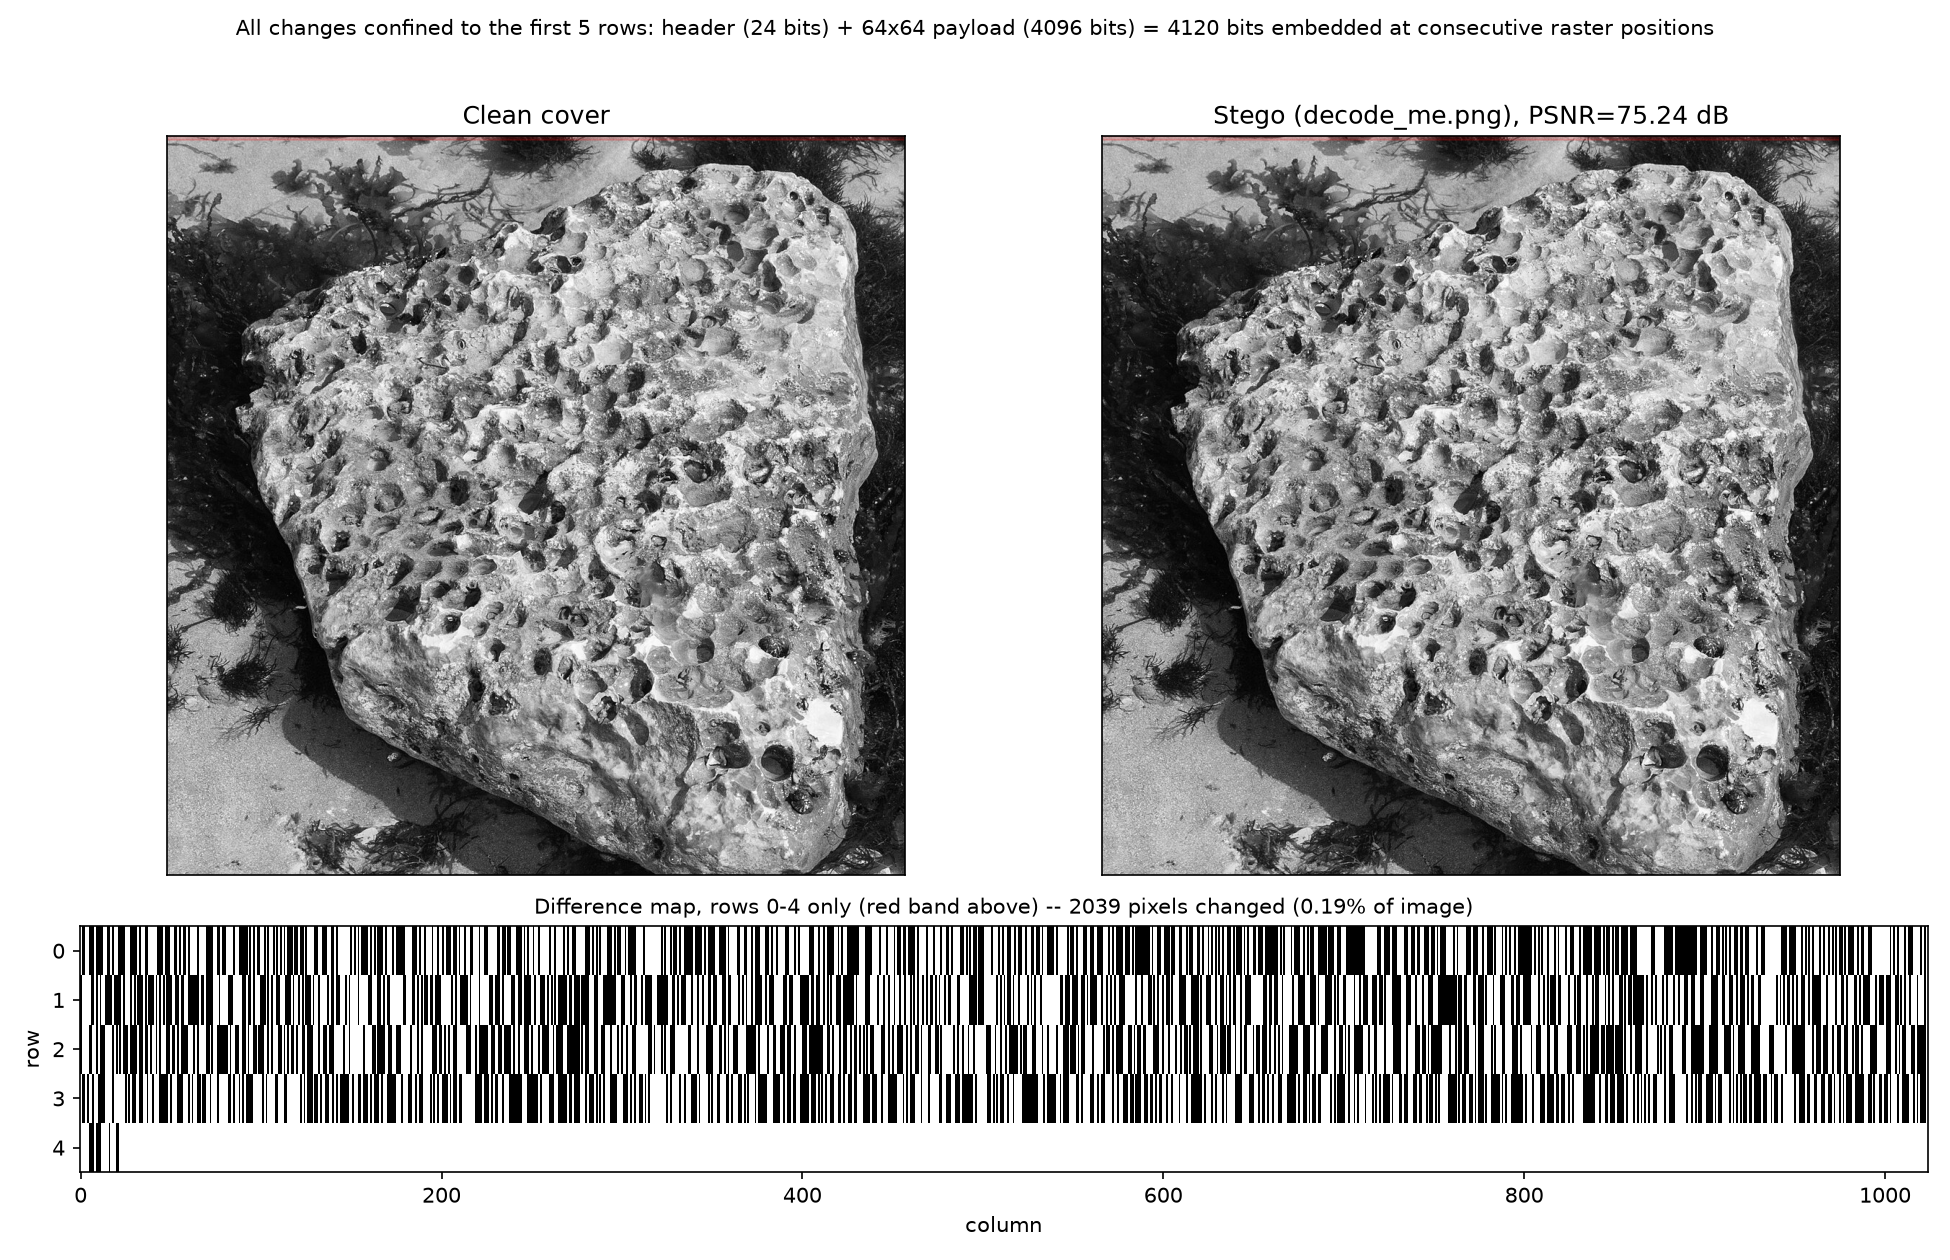
\includegraphics[width=\textwidth]{Images/p2_2_2_stego_diff.png}
\caption{Clean cover and stego image (red band marks where all 2039 of 1{,}048{,}576 changed
pixels, 0.19\%, are located --- invisible at this scale); bottom strip zooms into exactly those
rows, showing the embedded bit pattern directly. All changes fall in rows 0--4 because the 4120
header+payload bits are written at consecutive raster positions starting from the top-left.}
\label{fig:stego_diff}
\end{figure}
PSNR(stego, clean cover) $= 75.24$\,dB. At this PSNR and with only $0.19\%$ of pixels perturbed
by a single grey level, the payload is not visible by eye --- a single-LSB change is far below
the just-noticeable difference for natural images, and the difference map (right panel) shows no
structure recognisable as the payload shape without being told where to look.

\paragraph{Textured vs.\ smooth cover.}
The same $256\times256$-bit payload (65{,}536 payload bits plus the 24-bit header) was embedded
at identical raster positions into both \texttt{cover\_textured.png} and
\texttt{cover\_smooth.png}. PSNR is $63.20$\,dB for \emph{both} covers --- identical to two
decimal places, confirming the handout's point that PSNR is nearly cover-independent for a fixed
count of one-level changes (MSE depends only on how many pixels were flipped by 1 grey level, not
on what those pixels' neighbourhoods look like).

To distinguish the two covers, the local $5\times5$ standard deviation of each cover was measured
at every changed pixel:

\begin{table}[H]
\centering
\begin{tabular}{lcc}
\toprule
& \texttt{cover\_textured} & \texttt{cover\_smooth} \\
\midrule
Mean local std at changed pixels & 16.44 & 3.57 \\
Median local std at changed pixels & 11.05 & 3.39 \\
\bottomrule
\end{tabular}
\caption{Local $5\times5$ neighbourhood standard deviation (grey levels) at the positions the
embedding actually changed.}
\end{table}

\begin{figure}[H]
\centering
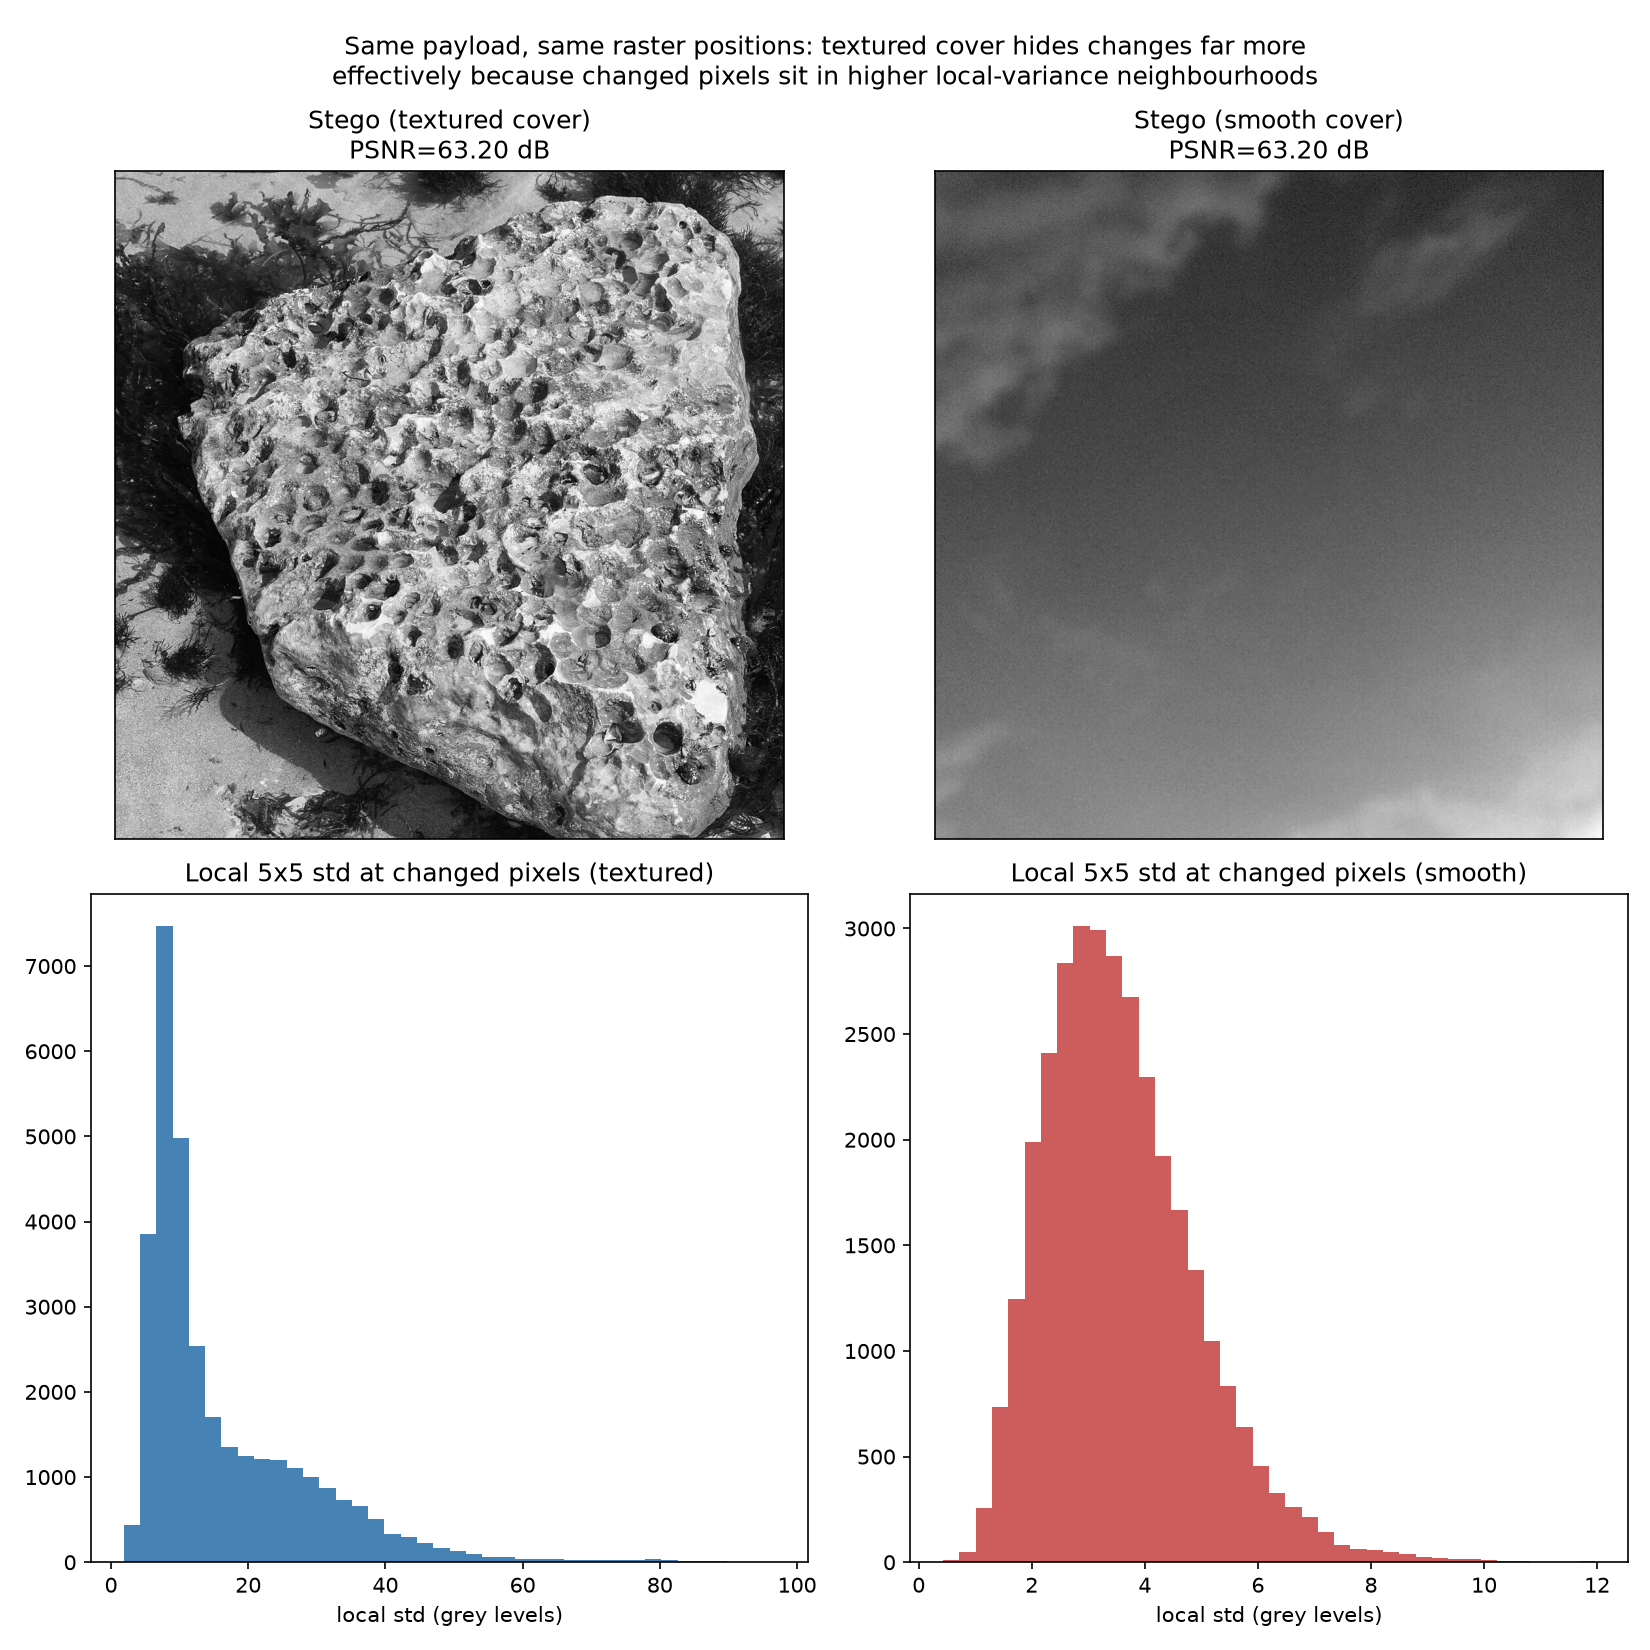
\includegraphics[width=0.75\textwidth]{Images/p2_2_2_textured_vs_smooth.png}
\caption{Stego images and the distribution of local standard deviation at changed pixels, for
both covers.}
\label{fig:textured_vs_smooth}
\end{figure}

In \texttt{cover\_smooth}, a changed pixel's local neighbourhood has $\approx4.6\times$ less
natural variability (std $\approx3.6$ vs.\ $\approx16.4$ grey levels), so a 1-level LSB flip is a
much larger fraction of the local signal --- easier to detect statistically (e.g.\ by a
noise/variance-based steganalysis filter) and closer to visually perceptible in flat regions,
where the eye is more sensitive to small deviations than in high-texture regions. PSNR alone
cannot show this because it is a global, per-pixel-squared-error average that is blind to where
the changes land relative to local image structure; \texttt{cover\_textured} is the
materially better hiding place.

\subsection{2.3 Survive the channel (10)}

\paragraph{Naive LSB baseline.} As stated in the handout, naive plane-0 LSB embedding is already
at chance: measured BER $\ge 0.45$ at every $\sigma \ge 1$ tested and $0.555$ after JPEG-75
(Table~\ref{tab:ber_results}), because a $\pm1$-level LSB change is far below both the Gaussian
noise floor and the quantisation step JPEG applies to spatial-domain content.

\paragraph{Design: block-mean quantisation-index modulation (QIM) with repetition.}
The $1024\times1024$ cover is partitioned into non-overlapping $16\times16$ blocks (4096 blocks
total). Each of the 128 message bits is assigned a disjoint run of $4096/128=32$ blocks; every
pixel in each assigned block is shifted by $+\delta$ (bit $=1$) or $-\delta$ (bit $=0$),
$\delta=2$ grey levels, clipped to $[0,255]$. To decode, each block's mean in the received image
is compared against its mean in the clean cover; a positive difference votes bit 1, negative
votes bit 0, and the 32 votes per bit are majority-combined.

Two independent averaging effects make this robust. First, by the central limit theorem,
averaging i.i.d.\ noise of standard deviation $\sigma$ over a $16\times16=256$-pixel block
reduces the noise seen by the block \emph{mean} to standard deviation $\sigma/16$; at the
required $\sigma=5$ this is an effective $\approx0.31$ on the block mean, tiny next to
$\delta=2$. Second, JPEG's luminance quantisation table allocates a much finer step to the DC coefficient
(proportional to the block mean) than to high-frequency AC coefficients --- a uniform
block-level shift survives JPEG-75 essentially intact, unlike single-pixel LSB parity. The 32-way majority vote adds a third, independent layer of margin on top of both
effects.

\paragraph{(a) Blind or cover-assisted.}
The submitted decoder is \textbf{cover-assisted}: it compares each block's stego mean against
its mean in the original cover to determine the sign of the shift. Removing this dependency
would require a decision rule computable from the stego image alone, e.g.\ quantising the block
mean to the nearest multiple of $2\delta$ from a fixed grid (true QIM/dither modulation) rather
than measuring a signed shift relative to an unknown original --- this trades some robustness
margin (the fixed grid must absorb all channel noise directly, with no cover reference to
subtract out the image's own local mean) for cover-independence, and was not required here since
the handout accepts either.

\paragraph{(b) Distortion budget.}
At the $\text{PSNR}\ge40$dB floor, the maximum allowed MSE is
$255^2/10^{4} = 6.50$, i.e.\ an RMS error budget of $\sqrt{6.50}\approx2.55$ grey levels per
pixel if \emph{every} pixel is modified (as in this design, where all $1024^2$ pixels are
shifted by exactly $\delta$). This design spends MSE $=\delta^2=4.0$ (PSNR $=42.11$dB), i.e.\
about 61\% of the available budget, banking the rest as margin -- consistent with the 0 BER
observed up to $\sigma=20$ (four times the required $\sigma=5$), not just at the required
threshold. Because 128 bits are spread over $2^{20}$ pixels, the floor is not the binding
constraint at all: even $\delta=2.55$ (using the entire budget) would touch every pixel by only
2--3 grey levels, invisible next to this cover's own texture (\S2.2 measured local std of tens
of grey levels in textured regions).

\paragraph{BER against $\sigma$, and JPEG-75.}
\begin{figure}[H]
\centering
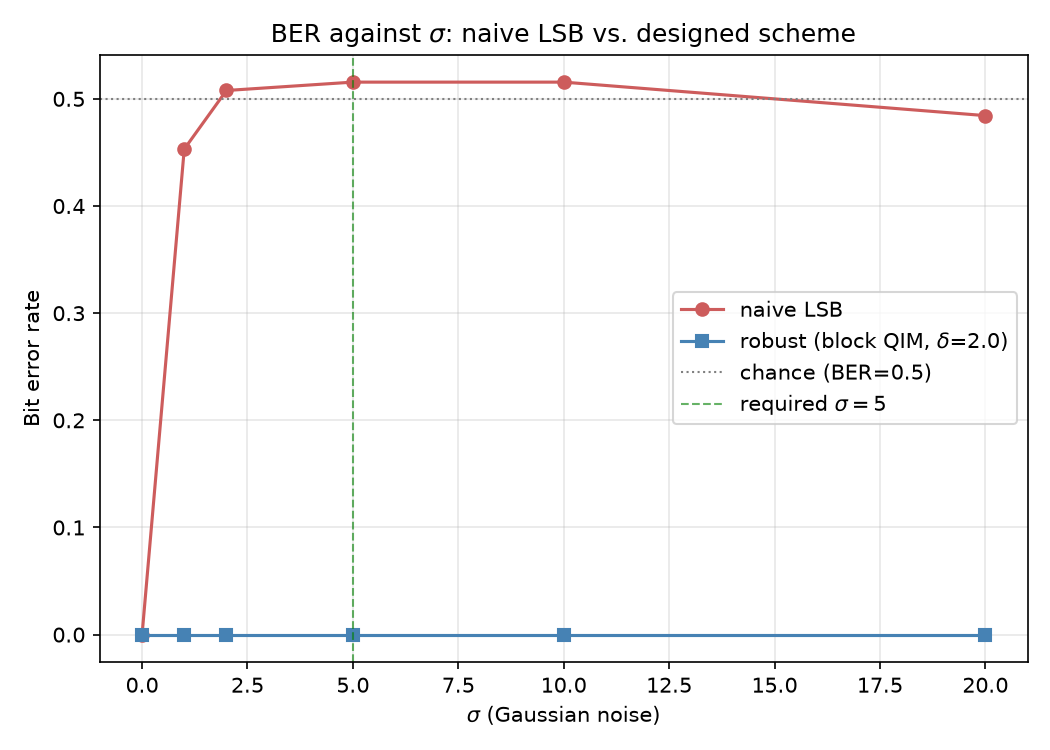
\includegraphics[width=0.75\textwidth]{Images/p2_2_3_ber_vs_sigma.png}
\caption{BER against $\sigma$ for naive LSB and the designed block-QIM scheme.}
\label{fig:ber_vs_sigma}
\end{figure}

\begin{table}[H]
\centering
\resizebox{\textwidth}{!}{% Auto-generated by run_2_3_robust.py -- do not edit by hand
\begin{tabular}{lcccccccc}
\toprule
Scheme & PSNR & $\sigma{=}0$ & $\sigma{=}1$ & $\sigma{=}2$ & $\sigma{=}5$ & $\sigma{=}10$ & $\sigma{=}20$ & JPEG75 \\
\midrule
Naive LSB & 90.28dB & 0.000 & 0.453 & 0.508 & 0.516 & 0.516 & 0.484 & 0.555 \\
Robust (ours) & 42.11dB & 0.000 & 0.000 & 0.000 & 0.000 & 0.000 & 0.000 & 0.000 \\
\bottomrule
\end{tabular}
}
\caption{PSNR, BER at each $\sigma\in\{0,1,2,5,10,20\}$, and JPEG-75 BER, for naive LSB and the
designed scheme (128-bit payload, \texttt{cover\_textured.png}).}
\label{tab:ber_results}
\end{table}

The designed scheme achieves exactly 0 BER at every $\sigma$ tested (including the required
$\sigma=5$) and after JPEG-75, at PSNR $=42.11$dB $\ge40$dB, meeting the stated requirement with
margin on both the imperceptibility and robustness axes.

\paragraph{A rejected alternative: blind mid-frequency DCT differencing.}
A block-DCT scheme was also implemented and tested: partition the image into $64\times64$
regions (one per bit), and within each region's $8\times8$ blocks enforce a signed margin
$|C(3,2)-C(2,3)|\ge\Delta$ between two mid-frequency AC coefficients (chosen for a textbook
reason -- resistant to both Gaussian smoothing, which mainly attenuates high frequencies, and
JPEG's coarser quantisation of high-frequency AC content), decoding \emph{blindly} from the sign
of $\sum_{\text{blocks}}[C(3,2){-}C(2,3)]$ with no clean cover needed. This does reach 0 BER at
$\sigma=5$ and JPEG-75, but only at $\text{PSNR}=40.33$dB for $\Delta=10$ -- a $0.33$dB margin
above the floor, an order of magnitude thinner than the submitted design's $2.1$dB margin, and
uncomfortably close to failing the requirement outright under any additional measurement
variance. Investigating why revealed a deeper issue with the blindness claim itself: on the
\emph{unmodified} cover, the same statistic $\sum[C(3,2){-}C(2,3)]$ has mean $15.3$ but standard
deviation $\approx345$ across the 128 regions -- real image content already biases this
coefficient pair by an amount comparable to the embedding margin, so the "blind" zero threshold
is implicitly relying on this particular cover's coefficient statistics happening to wash out
under majority vote, not on a property guaranteed to hold for any image. This is the sense in
which a candidate can survive both required channels and still be the wrong design to submit:
passing both channels' BER = 0 tests once is necessary but not sufficient evidence of
robustness on this metric. This alternative was rejected in favour of the block-mean design's
larger, more legible safety margin.

\paragraph{Design justification.}
The scheme sits deliberately far towards the robustness/imperceptibility corner of the
capacity/robustness/imperceptibility triangle, away from capacity: 128 bits in $1024^2$ pixels
is a very low rate ($1.2\times10^{-4}$ bits/pixel), spent to buy a $32\times$ repetition code on
top of a per-block averaging effect that already suppresses noise by $16\times$ and a channel
(block DC) that JPEG barely touches. Imperceptibility is not sacrificed either --- PSNR is kept
comfortably clear of the 40dB floor with margin to spare, and the modification (a uniform
$\pm2$-level shift per block) produces no structured artefact, unlike concentrated single-pixel
changes. What is given up is exclusively payload size: this design could not scale to carrying
appreciably more than a few hundred bits at this block size without either shrinking $\delta$
(hurting robustness) or shrinking blocks/repetition (same trade), because both come directly out
of the same finite $1024\times1024$ pixel budget.

%=======================================================================
\section{Problem 3 --- Piecewise linear transforms (10)}
%=======================================================================

Method used throughout: for each input level $v$, \texttt{transfer\_curve} takes the mode of the
output values at pixels where \texttt{img\_in==v} as $\hat T[v]$, together with the supporting
pixel count $\texttt{cnt}[v]$. On every pair tested here the transform turned out to be exactly
deterministic (every pixel at a given input level maps to one identical output value, verified
directly), so the mode recovers $T[v]$ exactly wherever $\texttt{cnt}[v]>0$.
\texttt{fit\_piecewise} then finds, for each candidate segment count $k$, the exact optimal
placement of $k{-}1$ breakpoints (via dynamic programming over the supported levels, minimising
unweighted least-squares error --- unweighted because each \emph{level} is one independent fact
about $T$, not each pixel) and selects $k$ by a quantisation-floored BIC (derived in \S3.2).

\subsection{3.1 Recover two known transforms (4)}

\begin{figure}[H]
\centering
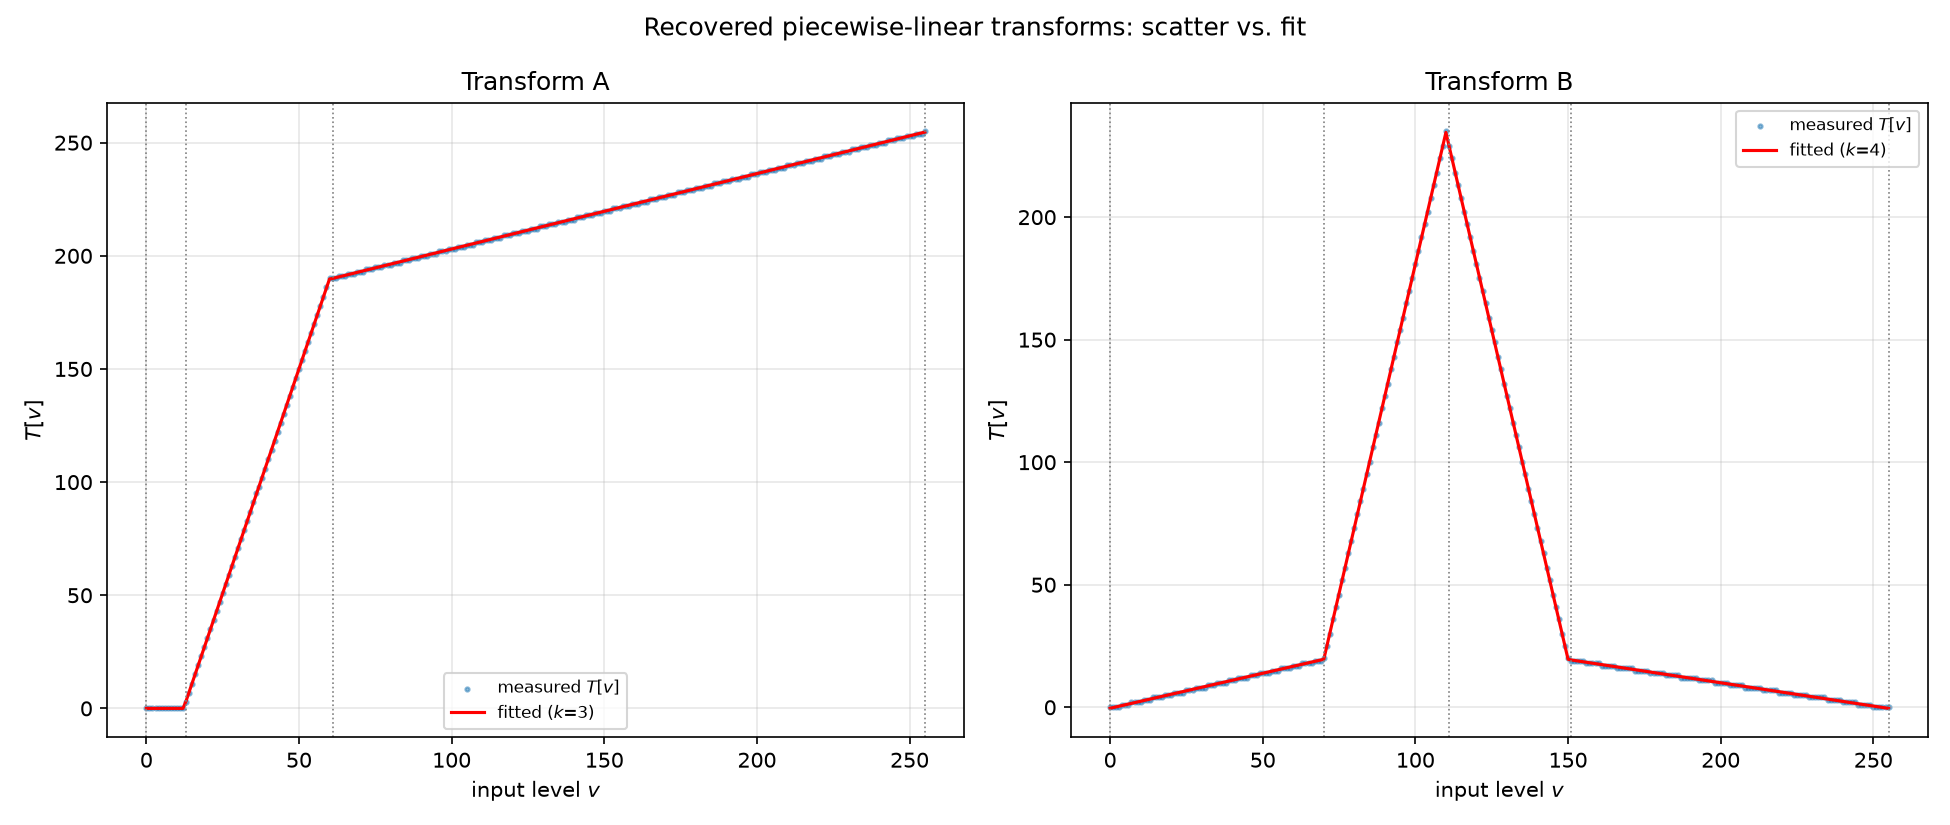
\includegraphics[width=\textwidth]{Images/p3_3_1_scatter_fit.png}
\caption{Measured $T[v]$ (scatter) and recovered piecewise-linear fit (red) for transforms A and
B, with fitted breakpoints marked.}
\label{fig:p3_scatter_fit}
\end{figure}

\begin{table}[H]
\centering
% Auto-generated by run_3_1_known_transforms.py -- do not edit by hand
\begin{tabular}{llccccc}
\toprule
Pair & Segment & Range $[v_{lo},v_{hi}]$ & Slope & Intercept & Max err & Mean err \\
\midrule
A & 1 & $[0,13]$ & 0.0000 & 0.00 & 0.000 & 0.00000 \\
A & 2 & $[13,61]$ & 3.9687 & -48.36 & -- & -- \\
A & 3 & $[61,255]$ & 0.3334 & 169.66 & -- & -- \\
B & 1 & $[0,70]$ & 0.2850 & -0.40 & 0.000 & 0.00000 \\
B & 2 & $[70,111]$ & 5.3746 & -356.64 & -- & -- \\
B & 3 & $[111,151]$ & -5.3729 & 825.54 & -- & -- \\
B & 4 & $[151,255]$ & -0.1901 & 48.03 & -- & -- \\
\bottomrule
\end{tabular}

\caption{Recovered breakpoints and slopes, and re-application error against the true output
(both exactly zero for both pairs).}
\label{tab:p3_breakpoints}
\end{table}

\textbf{A} recovers exactly $k=3$: a flat segment $[0,13]$ (slope 0, "flatten the sky floor"), a
steep rise $[13,61]$ (slope $\approx3.97$, "stretch the faint nebulosity"), and a shallow rise
$[61,255]$ (slope $\approx0.33$, "roll off the highlights") --- matching the handout's verbal
description exactly, monotonic throughout. \textbf{B} recovers $k=4$ and is clearly
\emph{non-monotonic}: slope rises to $+5.37$ then immediately falls to $-5.37$ (a symmetric tent
over $v\in[70,151]$), consistent with grey-level slicing that boosts a mid-tone band and
suppresses everything else. Re-applying each recovered transform to \texttt{field\_in.png}
reproduces the supplied output exactly (max and mean absolute error both $0.000$ for both pairs)
--- the dynamic program does not assume monotonicity anywhere, so it recovers B's tent shape with
the same machinery used for A's monotonic curve.

\textbf{B is recoverable from the pair but not invertible from the output alone} because it is
many-to-one (both $v\approx70$ and $v\approx151$ map to similar low output values): knowing only
$T(v)$ for a given $v$ tells you nothing about which of several possible pre-image bands $v$ came
from, whereas having both the input \emph{and} output image directly labels every pixel with its
$(v, T(v))$ pair, resolving the ambiguity by direct observation rather than by inverting a
non-injective function.

\subsection{3.2 Choose the number of segments (3)}

\paragraph{Complexity penalty.} A pure least-squares fit's SSE is monotonically non-increasing in
$k$ (more segments can only fit at least as well), so $k$ cannot be chosen by minimising SSE
alone. BIC, $n\log(\text{SSE}/n) + 2k\log n$ (2 free parameters --- slope, intercept --- per
segment; $n=$ number of \emph{supported levels}, not pixel count, since repeated pixels at one
level are the same observation of $T$ repeated, not independent evidence) trades fit quality
against the number of free parameters, penalising extra segments unless they earn their
complexity back in reduced error.

\paragraph{Selection for transform C.}
\begin{figure}[H]
\centering
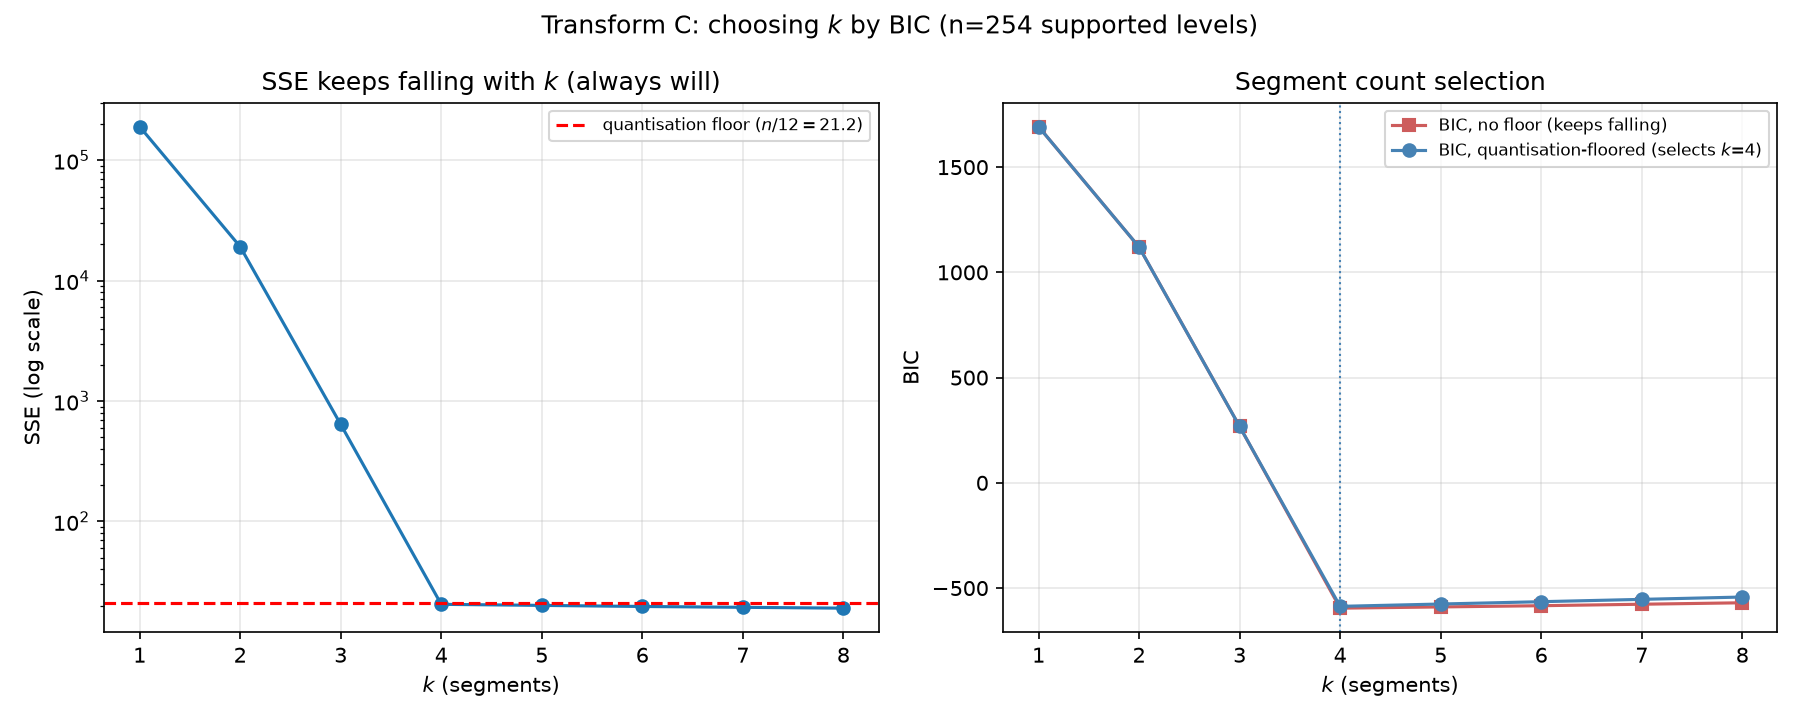
\includegraphics[width=0.85\textwidth]{Images/p3_3_2_bic_selection.png}
\caption{Transform C: SSE keeps falling with $k$ (left) but BIC bottoms out at $k=4$ (right);
$k=1..8$ tested, both floored and unfloored BIC agree here.}
\label{fig:p3_bic_C}
\end{figure}
BIC selects $k=4$ for transform C, with breakpoints $[1, 40, 121, 199, 255]$ and exact
re-application (max/mean error $0.000$, Figure~\ref{fig:p3_scatter_fit_C} below).

\begin{figure}[H]
\centering
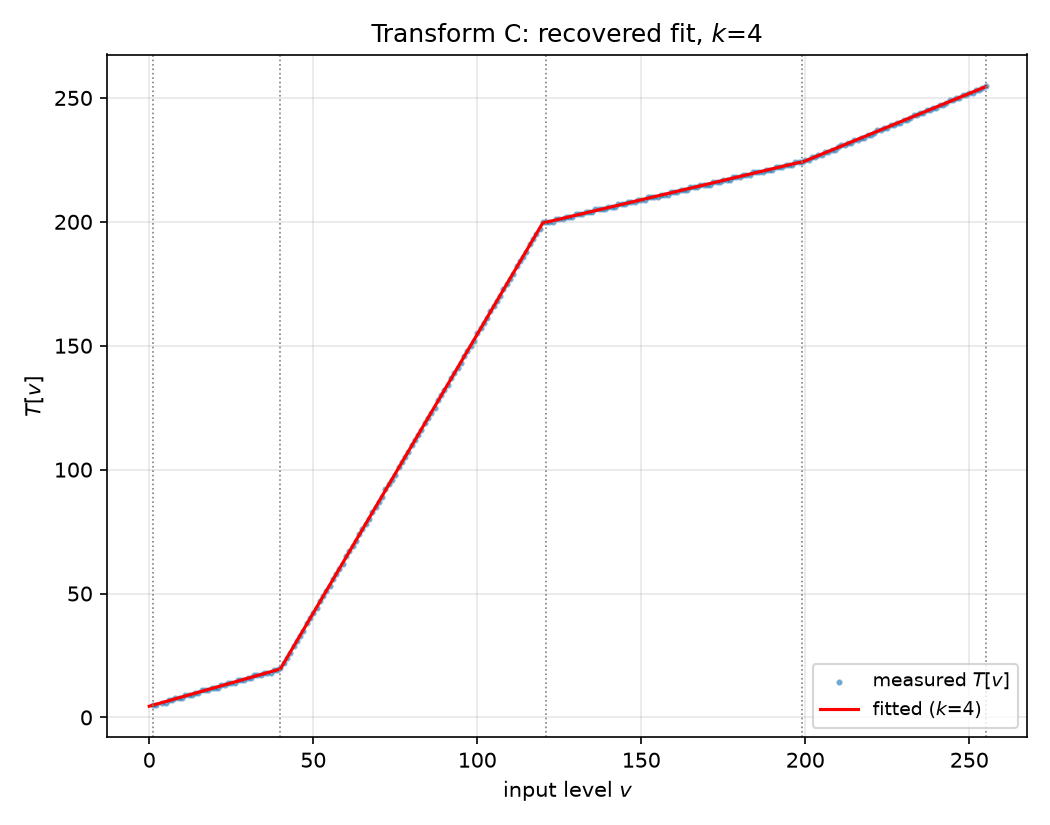
\includegraphics[width=0.6\textwidth]{Images/p3_3_2_scatter_fit_C.png}
\caption{Transform C: recovered $k=4$ fit.}
\label{fig:p3_scatter_fit_C}
\end{figure}

\paragraph{The quantisation-floor trap, demonstrated on transform A.}
Below some residual, a fit is no longer recovering the transform but the $\pm0.5$ rounding noise
of the 8-bit output LUT, and BIC's $\log(\text{SSE})$ term will happily reward chasing that noise
with more segments unless SSE is floored. The floor used is $n\cdot\tfrac1{12}$: the variance of
uniform $\pm0.5$ rounding noise per point, i.e.\ the best SSE any model can meaningfully achieve
once residuals are pure quantisation. Transform A (handout-stated true $k=3$) demonstrates the
failure mode directly:
\begin{figure}[H]
\centering
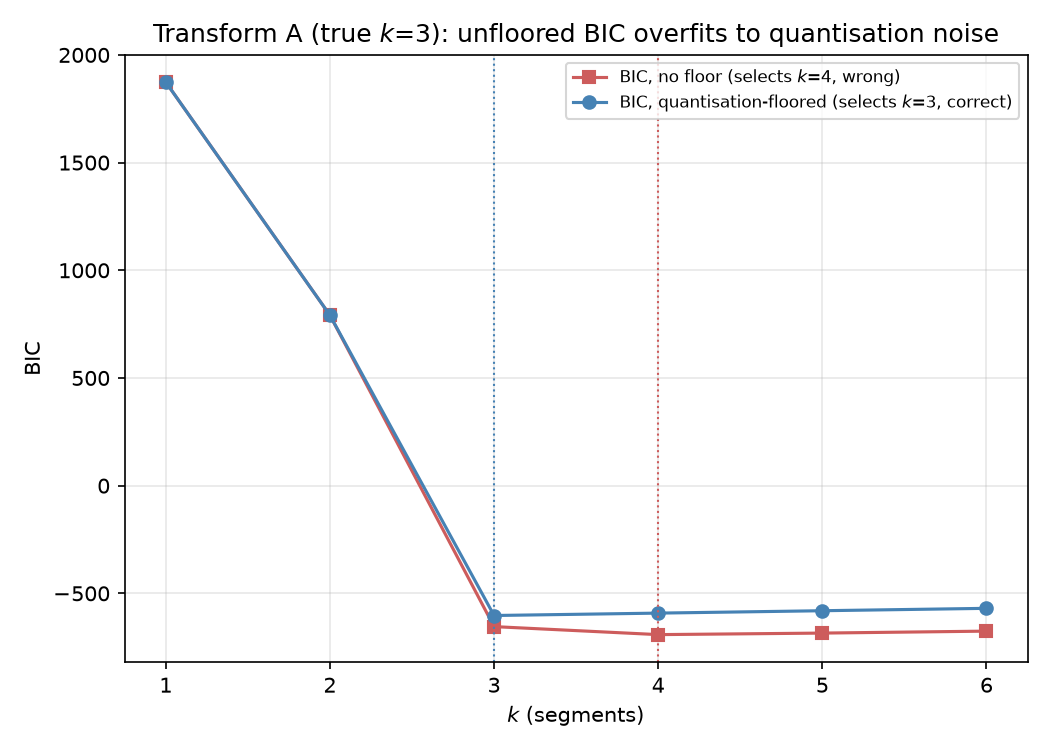
\includegraphics[width=0.7\textwidth]{Images/p3_3_2_quantisation_floor_demo.png}
\caption{Transform A: an unfloored BIC selects $k=4$ (wrong); the quantisation-floored BIC
selects $k=3$ (matches the handout).}
\label{fig:p3_quant_floor}
\end{figure}
Without the floor, BIC prefers $k=4$ (BIC $=-691.6$ vs.\ $k{=}3$'s $-654.5$) by splitting the
true middle segment $[13,60]$ into two pieces, $[13,36]$ and $[37,60]$, with slopes $3.9687$ and
$4.0000$ respectively --- near-identical integer-adjacent slopes fitting quantisation, not a real
second breakpoint, the failure mode the handout warns about.
With the floor applied, SSE at $k{=}3$ ($17.4$) is already below the floor $n/12\approx21.3$, so
flooring caps how much further $\log(\text{SSE})$ can fall; the $k$-dependent parameter penalty
then correctly makes $k=4$ worse ($-591.8$) than $k=3$ ($-602.9$), recovering the true 3-segment
structure with no near-duplicate slopes.

\subsection{3.3 Identifiability (3)}

\paragraph{(a) Input histogram and sampled range.}
\texttt{field\_skycrop\_in.png} is a $200\times200$ crop containing almost nothing but sky.
\begin{figure}[H]
\centering
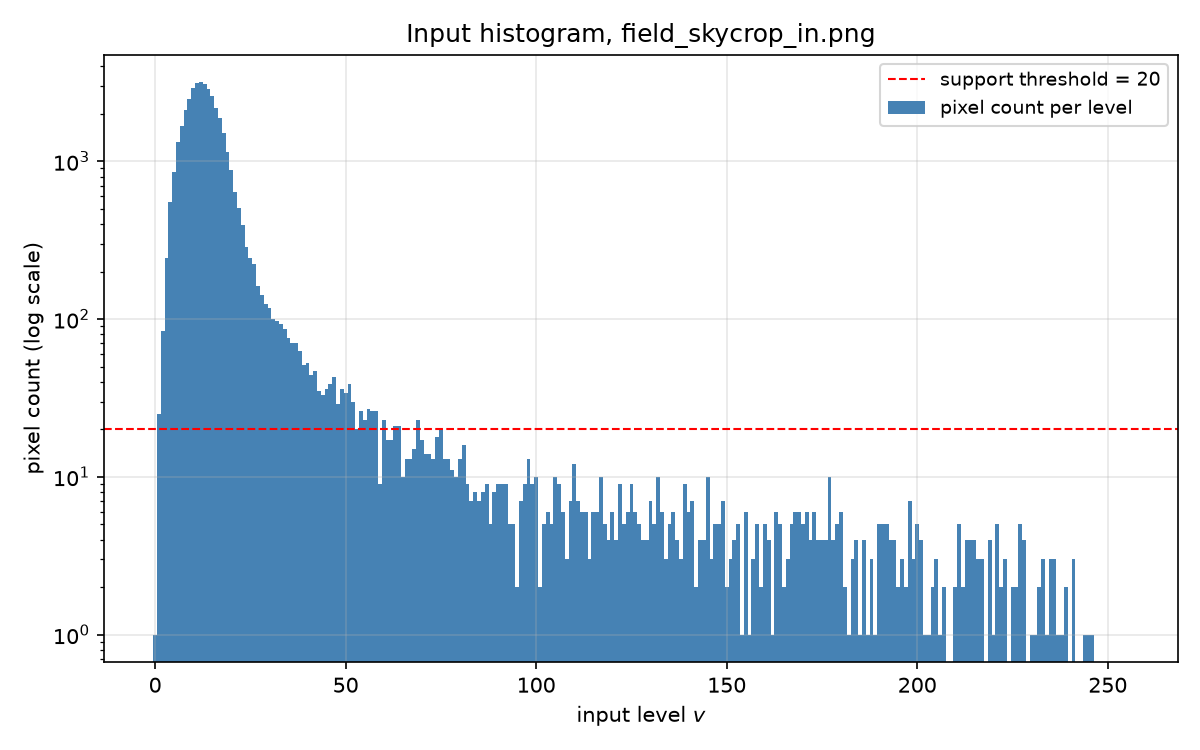
\includegraphics[width=0.75\textwidth]{Images/p3_3_3_input_histogram.png}
\caption{Input histogram (log scale), support threshold $\texttt{cnt}\ge20$ marked.}
\label{fig:p3_histogram_D}
\end{figure}
Sampled input levels span $[0,246]$, but the distribution is extremely peaked: a dense mode
around $v\approx10$--$20$ (thousands of pixels/level) falling to a long tail from $v\approx76$ to
$246$ where most levels have single-digit pixel counts, with several levels entirely unsampled
(e.g.\ $v\in\{208,209,218,224,229,240,242,243\}$ and all of $[247,255]$). The threshold
$\texttt{cnt}\ge20$ was chosen because it sits at the natural knee of the histogram
(Figure~\ref{fig:p3_histogram_D}): it is comfortably above the noisy single-digit tail while
retaining every level in the dense sky-floor mode, and is large enough that a level's mode-value
estimate is not just one or two lucky/unlucky pixels.

\paragraph{(b) What the data supports.}
Restricting \texttt{fit\_piecewise} to only the trusted levels ($\texttt{cnt}\ge20$, contiguous
range $[1,75]$) recovers $k=3$: breakpoints $[1, 21, 56, 75]$, slopes $[1.50, 4.86, 0.33]$.
\begin{figure}[H]
\centering
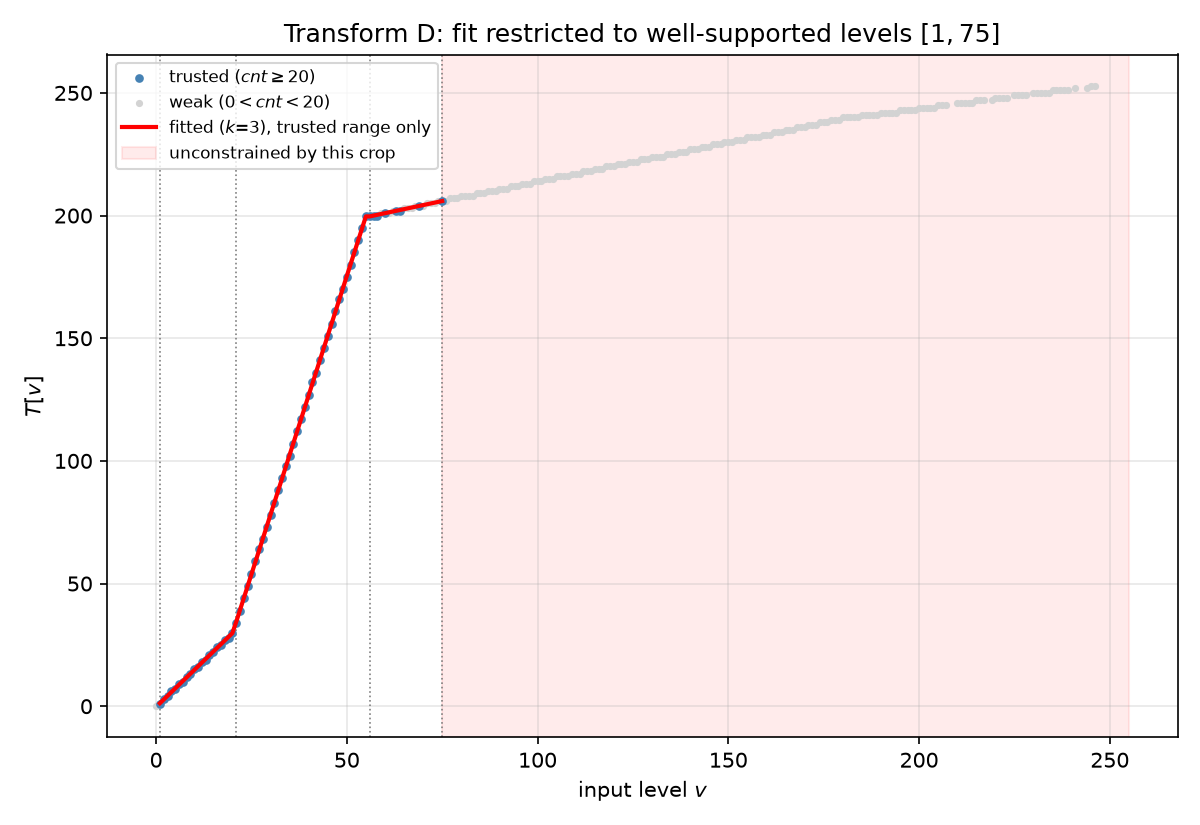
\includegraphics[width=0.75\textwidth]{Images/p3_3_3_scatter_fit_D.png}
\caption{Fit restricted to trusted levels $[1,75]$ (blue points, red fitted curve); weak-support
points ($0<\texttt{cnt}<20$, grey) are shown but not fitted; the shaded band $v>75$ is
unconstrained by this crop.}
\label{fig:p3_scatter_fit_D}
\end{figure}
The two recovered breakpoints ($v\approx21$, $v\approx56$) and their slopes closely match the
first two segments of transform A recovered from the full-frame pair in \S3.1 (breakpoints 13 and
61, slopes 0/3.97), consistent with D's true transform being related to A's and confirming the
trusted-only fit recovered real structure rather than an artefact. For contrast, a naive fit using
every \emph{supported} level (ignoring the support threshold entirely) reports $k=4$ with a
spurious extra breakpoint at $v=177$, built almost entirely on levels with 1--10 supporting
pixels each --- a fabricated-looking but unjustified 4th segment, the mistake the threshold in (a)
exists to prevent. \textbf{The intensity range $v\in(75,255]$ is
unconstrained by this crop}: individual pixels do exist out there (the grey points in
Figure~\ref{fig:p3_scatter_fit_D} trace a smooth-looking curve all the way to $v\approx246$), but
each level has too few supporting pixels to distinguish a real breakpoint from a single noisy or
unrepresentative sample --- the smooth appearance of the untrusted tail is itself the trap: it
looks fittable, but no other curve agreeing with the trusted region and disagreeing only past
$v=75$ can be ruled out by this data.

\paragraph{(c) Why 3, not the stated true 4.}
3 segments were reported, not 4, because only the input levels up to $v\approx75$ are sampled
densely enough to trust $T[v]$ there; the crop is almost pure sky, so it simply does not contain
enough highlight-range pixels to constrain whatever segment(s) exist beyond that level. This is
not a limitation of the fitting method --- \S3.1 showed the same dynamic program recovers all 3
segments of A and all 4 (non-monotonic) segments of B \emph{exactly} when the input image
actually samples the full range. Reporting 4 segments here would mean fitting a breakpoint to
data that contains, at some levels, literally zero supporting pixels and at others only a
handful; recognising that no amount of algorithmic sophistication recovers a parameter the data
does not constrain is the correct answer, not a failure to find one more segment.

%=======================================================================
\section{Problem 4 --- Histograms (25)}
%=======================================================================

\subsection{4.1 Global equalisation (5)}

$T(v)=\text{round}(255F(v))$, $F$ the normalised inclusive CDF, no $\text{CDF}_{\min}$ rescaling.

\begin{figure}[H]
\centering
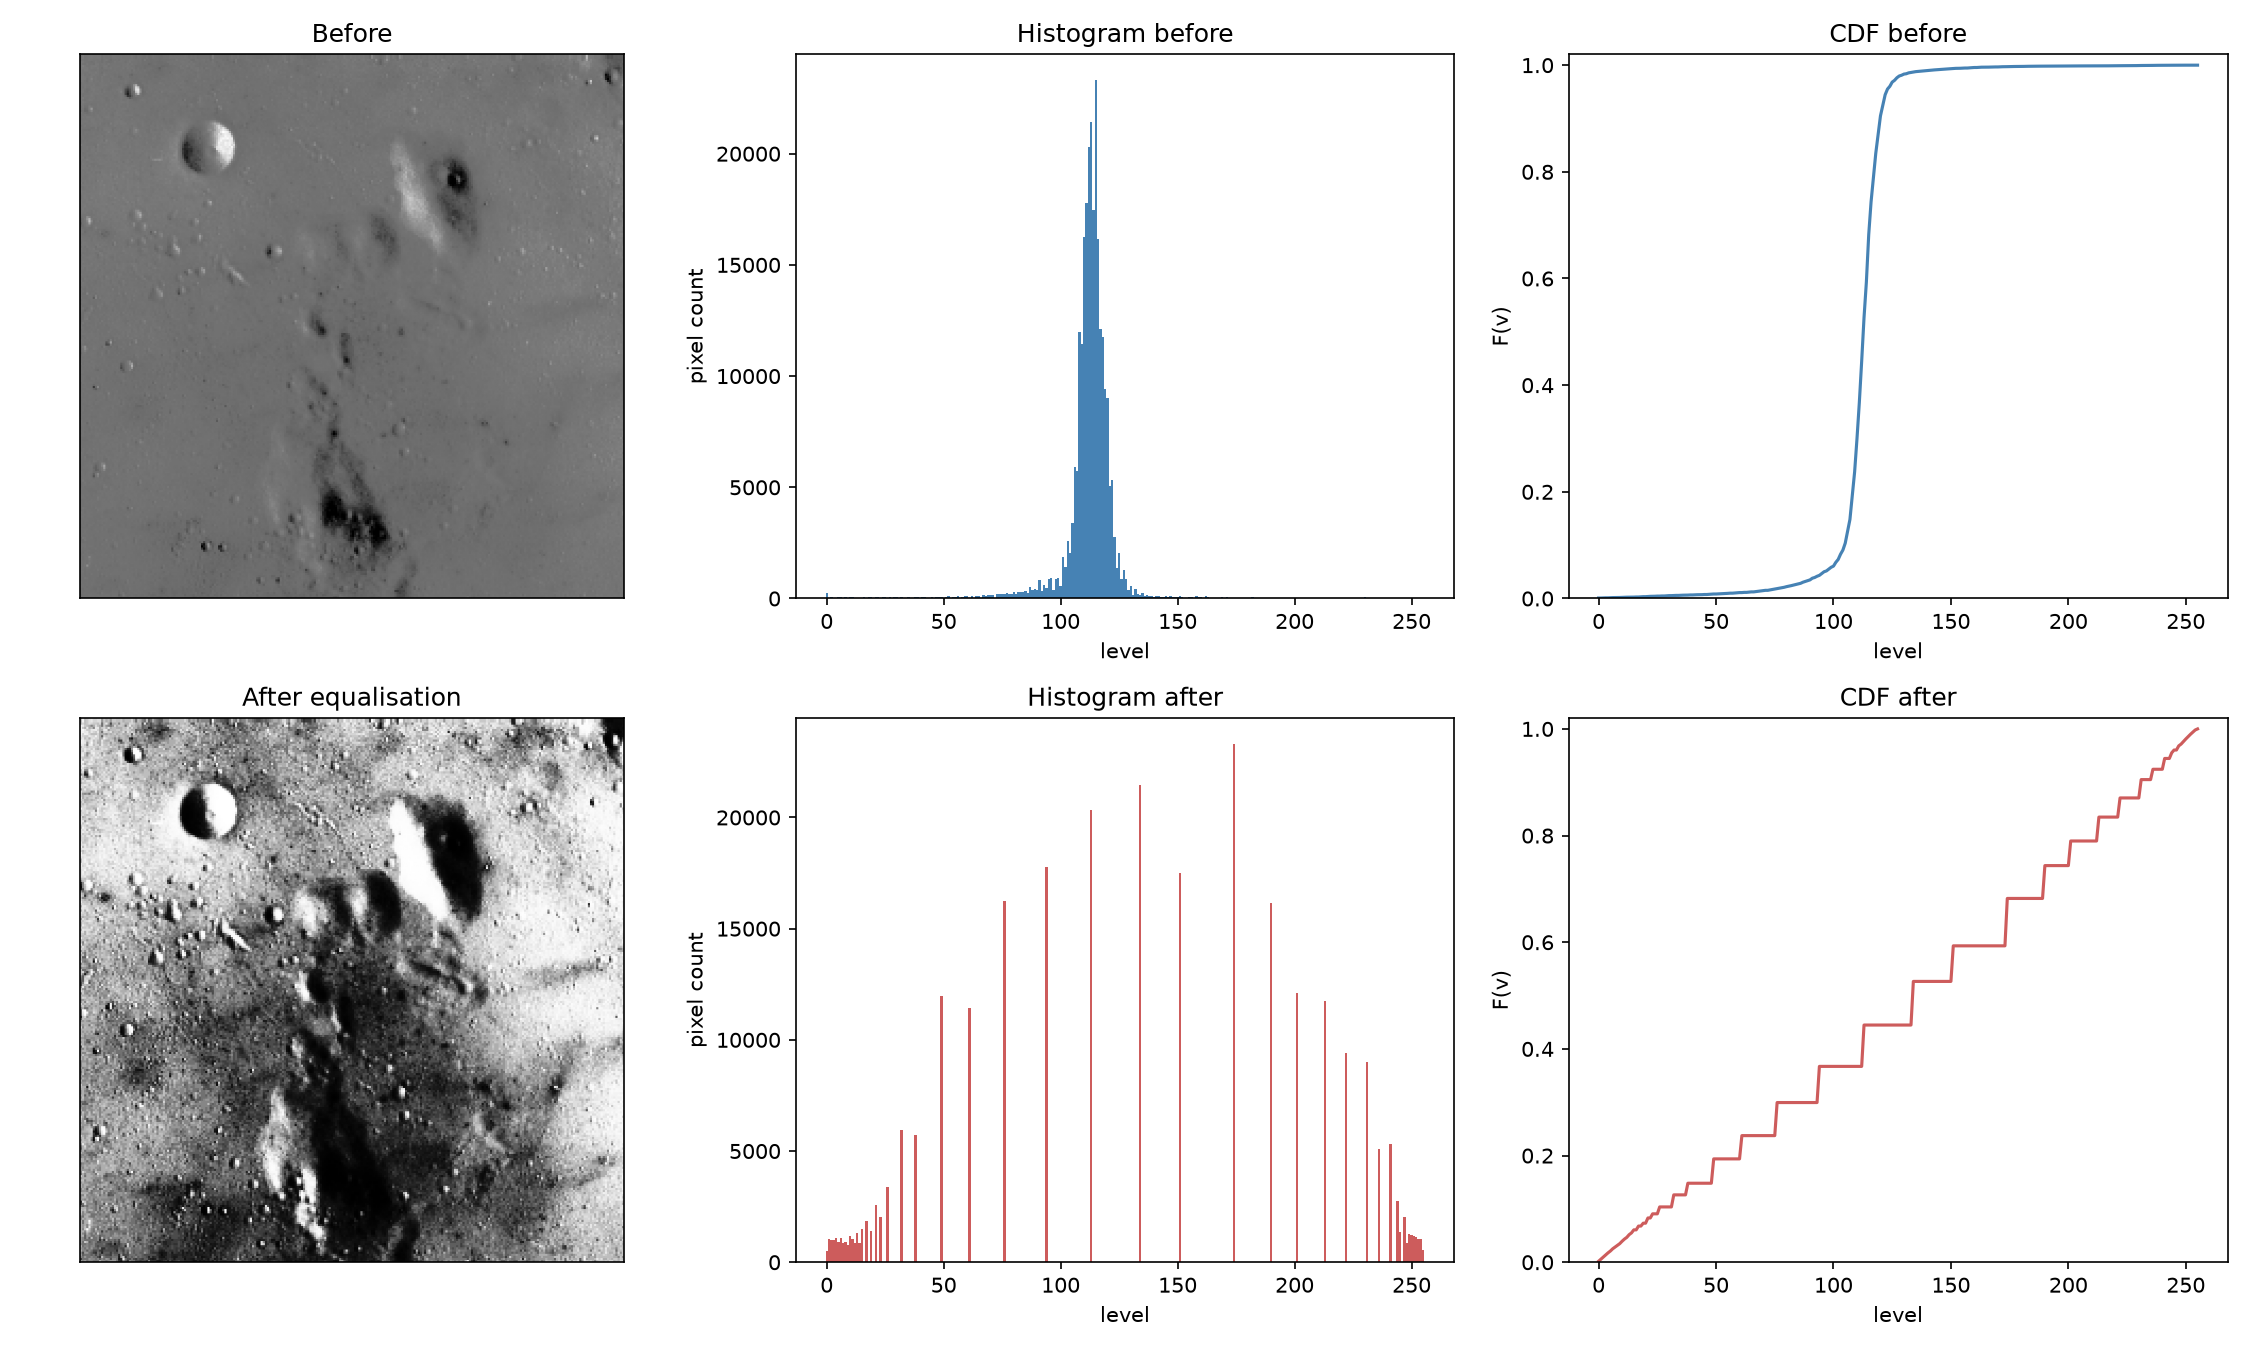
\includegraphics[width=\textwidth]{Images/p4_4_1_before_after.png}
\caption{\texttt{equalization/input.png} before/after equalisation, with histograms and CDFs.}
\label{fig:p4_before_after}
\end{figure}

\paragraph{(a) The equalised histogram cannot be flat.}
$T$ maps the (at most 256) distinct input levels to output levels via rounding a monotonic,
piecewise-constant CDF; it is a many-to-one, integer-valued step function. A perfectly flat
output histogram would require every one of the 256 output bins to receive exactly $N/256$
pixels, for arbitrary $N$ and an arbitrary input distribution. But $T$ can only \emph{merge}
input levels into shared output bins (whenever $F$ is near-constant across levels, several $v$'s
round to the same $w$) or leave gaps (whenever $F$ jumps by more than $1/255$ at one level, the
intermediate output levels get zero pre-images) --- it cannot subdivide a single input level's
pixel mass across multiple output bins. Any input level $v$ with $h(v) \ne N/256$ therefore dumps
its entire (generically unequal) pixel count into one output bin, so the output histogram
inherits the lumpiness of the input's actual level populations wherever $T$ is locally
one-to-one, and produces spikes/gaps wherever $T$ is not. Only an input whose histogram is
\emph{already} uniform escapes this (\S4.1(c)); a generic photograph is not.

\paragraph{(b) Equalisation is exactly idempotent.}
Let $T(v)=\text{round}(255F(v))$ from image $I$, and $I'=T(I)$. Because $F$ is non-decreasing,
$T$ is non-decreasing, so the pre-image of each output level $w$ under $T$ is a contiguous block
of input levels; let $v_w=\max\{v : T(v)=w\}$ be the top of that block (for $w$ that actually
occur in $I'$). Equalising $I'$ again uses $I'$'s own CDF $F'$; because $T$ only merges
contiguous input levels into output bins without redistributing pixel mass, $F'(w)=F(v_w)$ for
every occurring $w$ --- the cumulative pixel count up to and including bin $w$ in $I'$ equals the
cumulative pixel count up to and including level $v_w$ in $I$, since exactly the pixels with
$v\le v_w$ landed in output bins $\le w$. Applying the same LUT formula to $I'$ therefore gives
$\text{round}(255F'(w)) = \text{round}(255F(v_w)) = T(v_w) = w$ for every $w$ that occurs, by the
definition of $v_w$ as (one of) the input level(s) mapping to $w$. So $T$ applied to $I'$ is the
identity on every level $I'$ actually contains: $\text{equalise}(\text{equalise}(I)) =
\text{equalise}(I)$ exactly. Verified numerically on \texttt{input.png}:
$\max|\text{equalise}(\text{equalise}(I)) - \text{equalise}(I)| = 0$ (bit-identical).

\paragraph{(c) An image on which equalisation does essentially nothing.}
If a histogram is already (close to) uniform, $F(v)\approx v/255$ and $T(v)=\text{round}(255F(v))
\approx v$: equalisation is close to the identity, because there is no lumpiness for it to
redistribute (per part (a), $T$ can only act by merging/spacing levels to compensate for uneven
pixel counts per level; if counts are already even, there is nothing to compensate for).
Constructed example: a $256\times256$ image with the integers $0..255$ each appearing exactly
$256$ times, positions shuffled at random.
\begin{figure}[H]
\centering
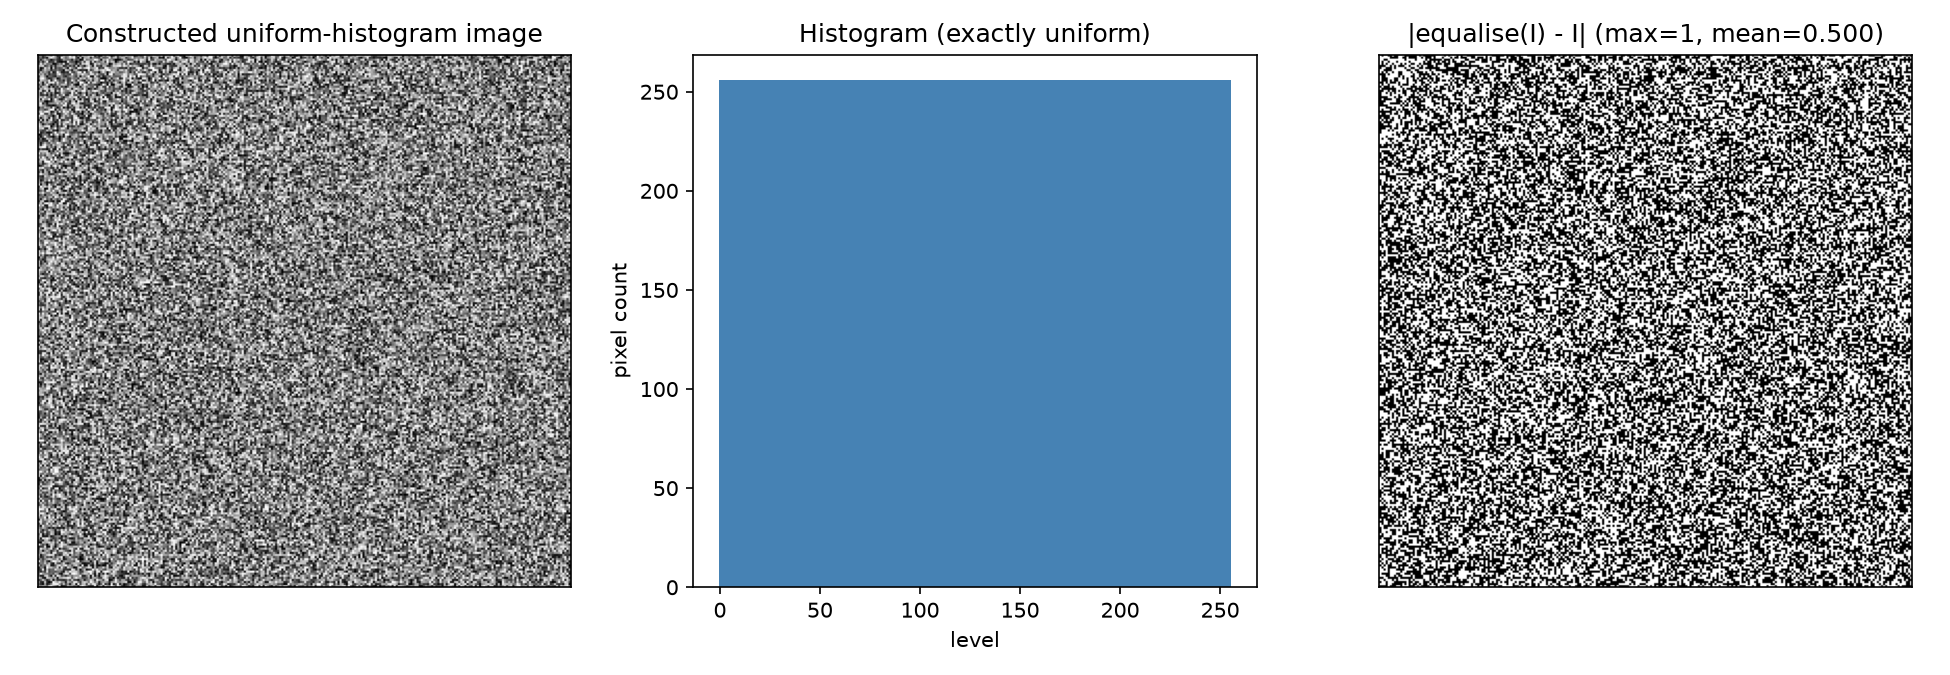
\includegraphics[width=0.9\textwidth]{Images/p4_4_1_near_noop.png}
\caption{Constructed exactly-uniform-histogram image: equalisation changes at most 1 grey level
per pixel (pure integer-rounding artefact), mean absolute change $0.5$.}
\label{fig:p4_near_noop}
\end{figure}

\subsection{4.2 Histogram matching and specification (6)}

\texttt{specify} implements inverse-CDF composition: for source level $v$, the output level is
the smallest $w$ with $F_{\text{target}}(w) \ge F_{\text{source}}(v)$ --- the standard
generalised-inverse construction, working from any prescribed 256-bin target distribution (not
necessarily from a real image).

\paragraph{(a) Image matching.}
\begin{figure}[H]
\centering
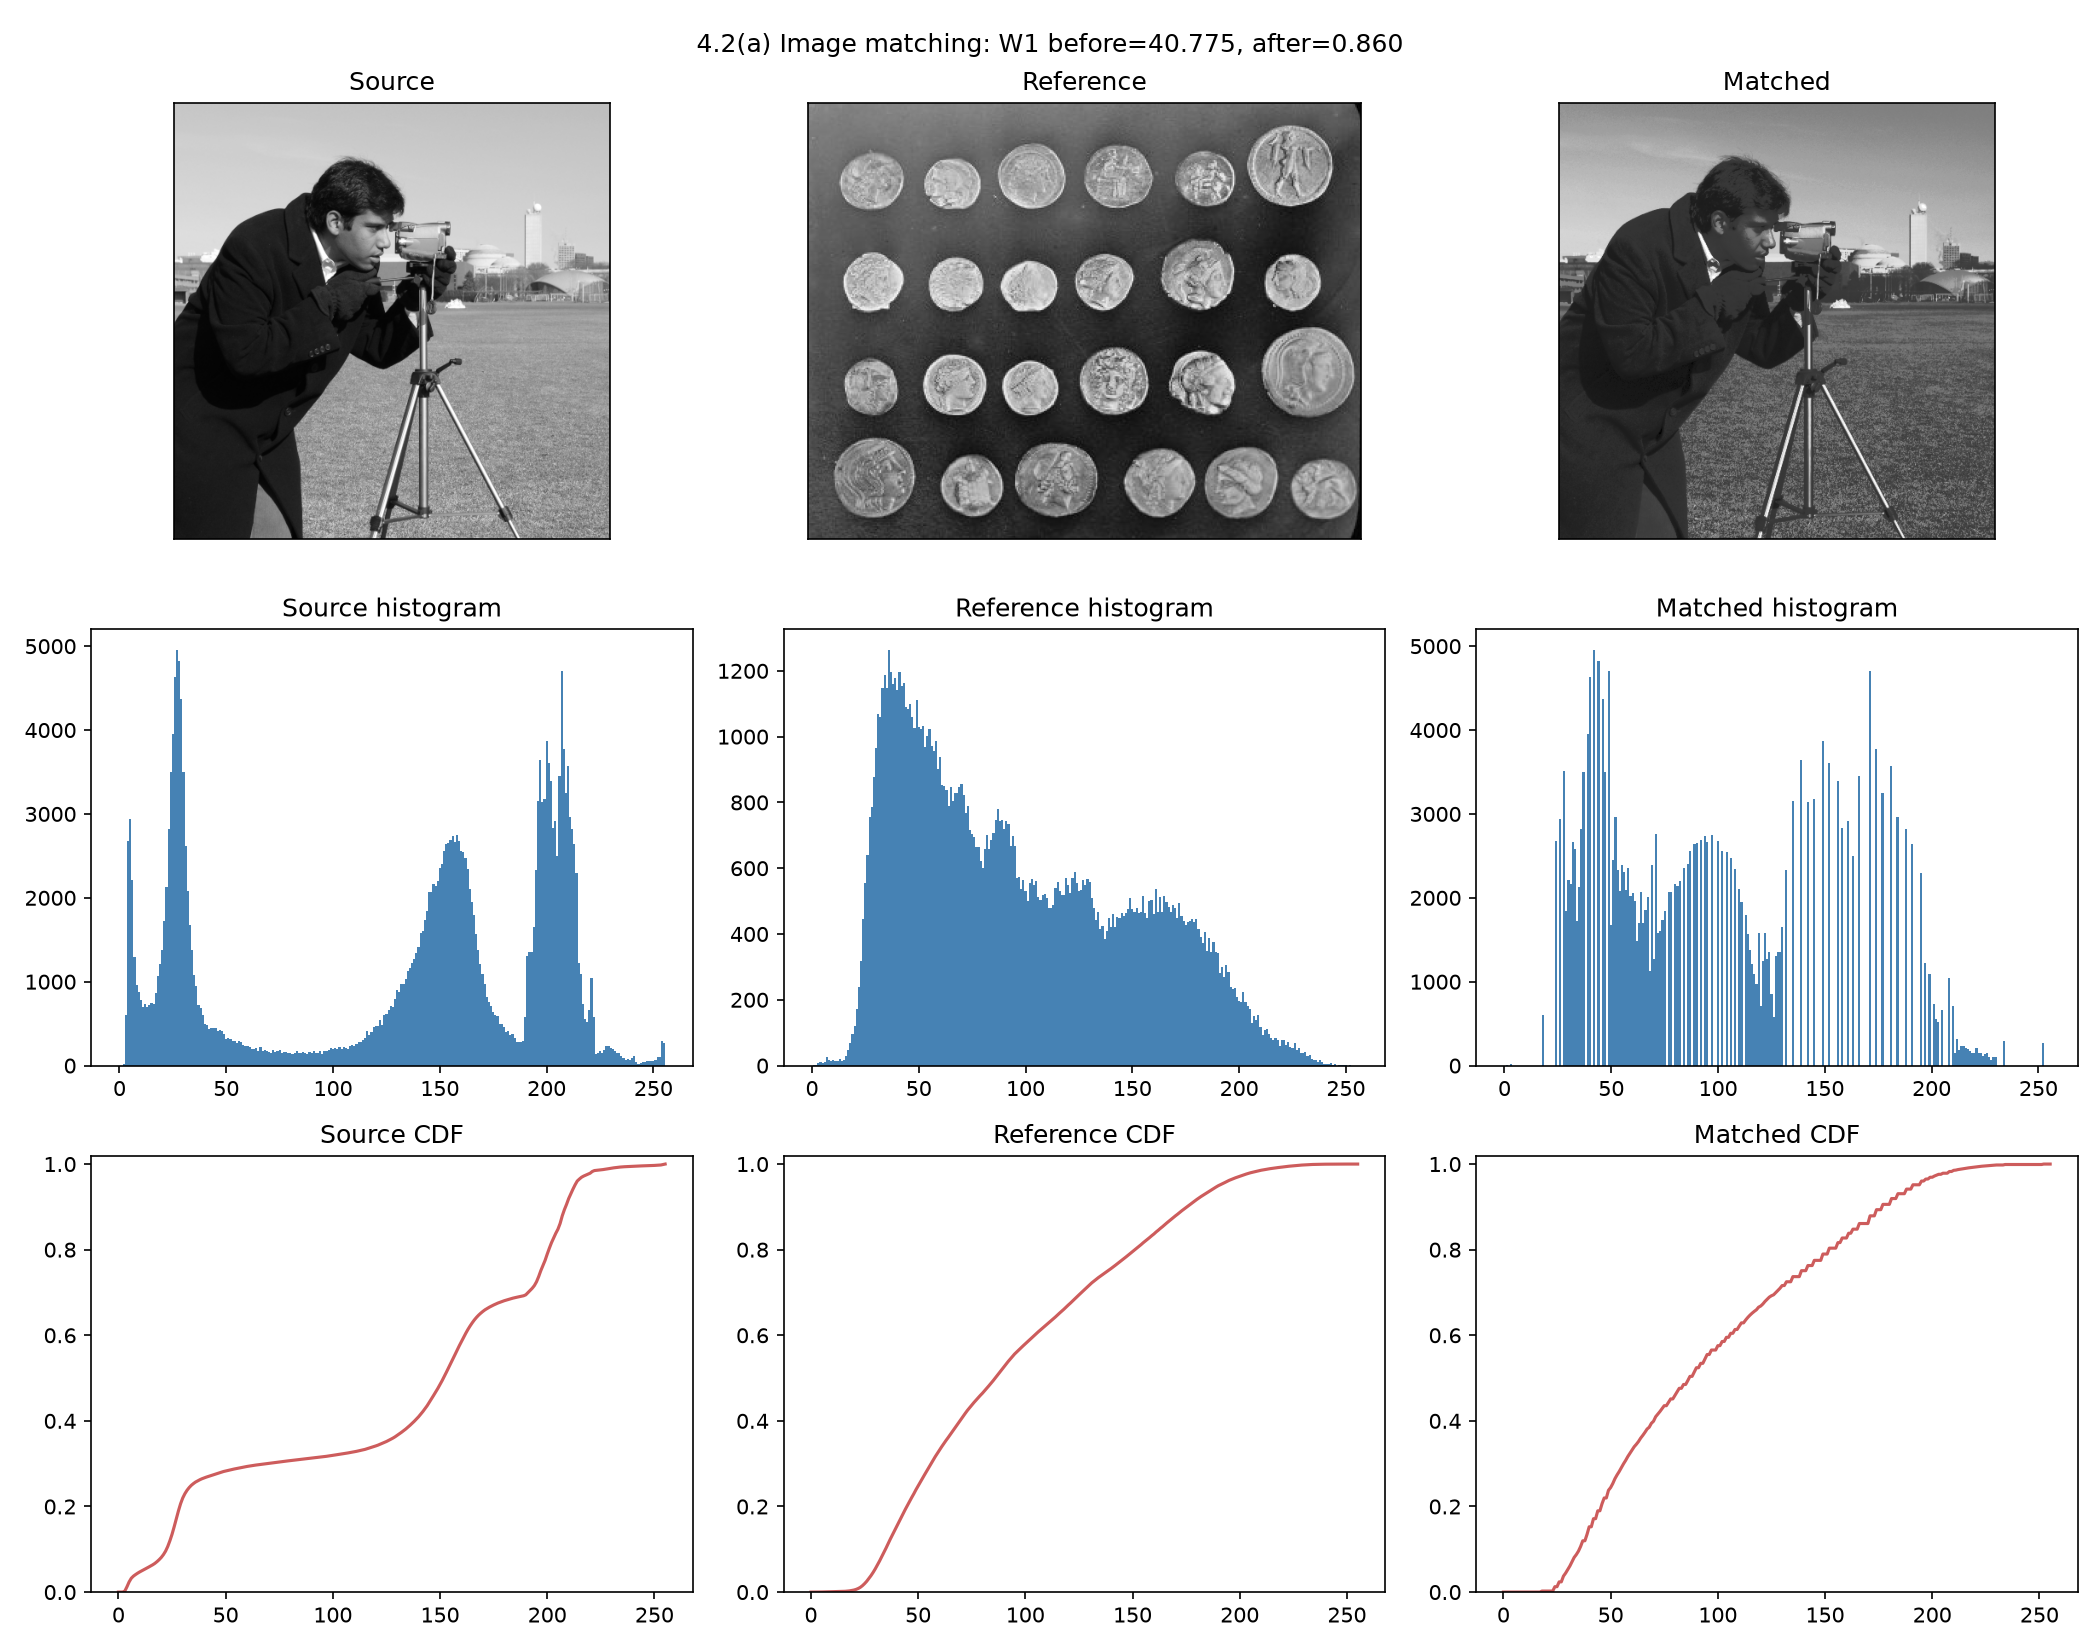
\includegraphics[width=\textwidth]{Images/p4_4_2_matching.png}
\caption{\texttt{matching/source.png} matched to \texttt{matching/reference.png}'s histogram.}
\label{fig:p4_matching}
\end{figure}

\paragraph{(b) Histogram specification: uniform and Gaussian targets.}
\begin{figure}[H]
\centering
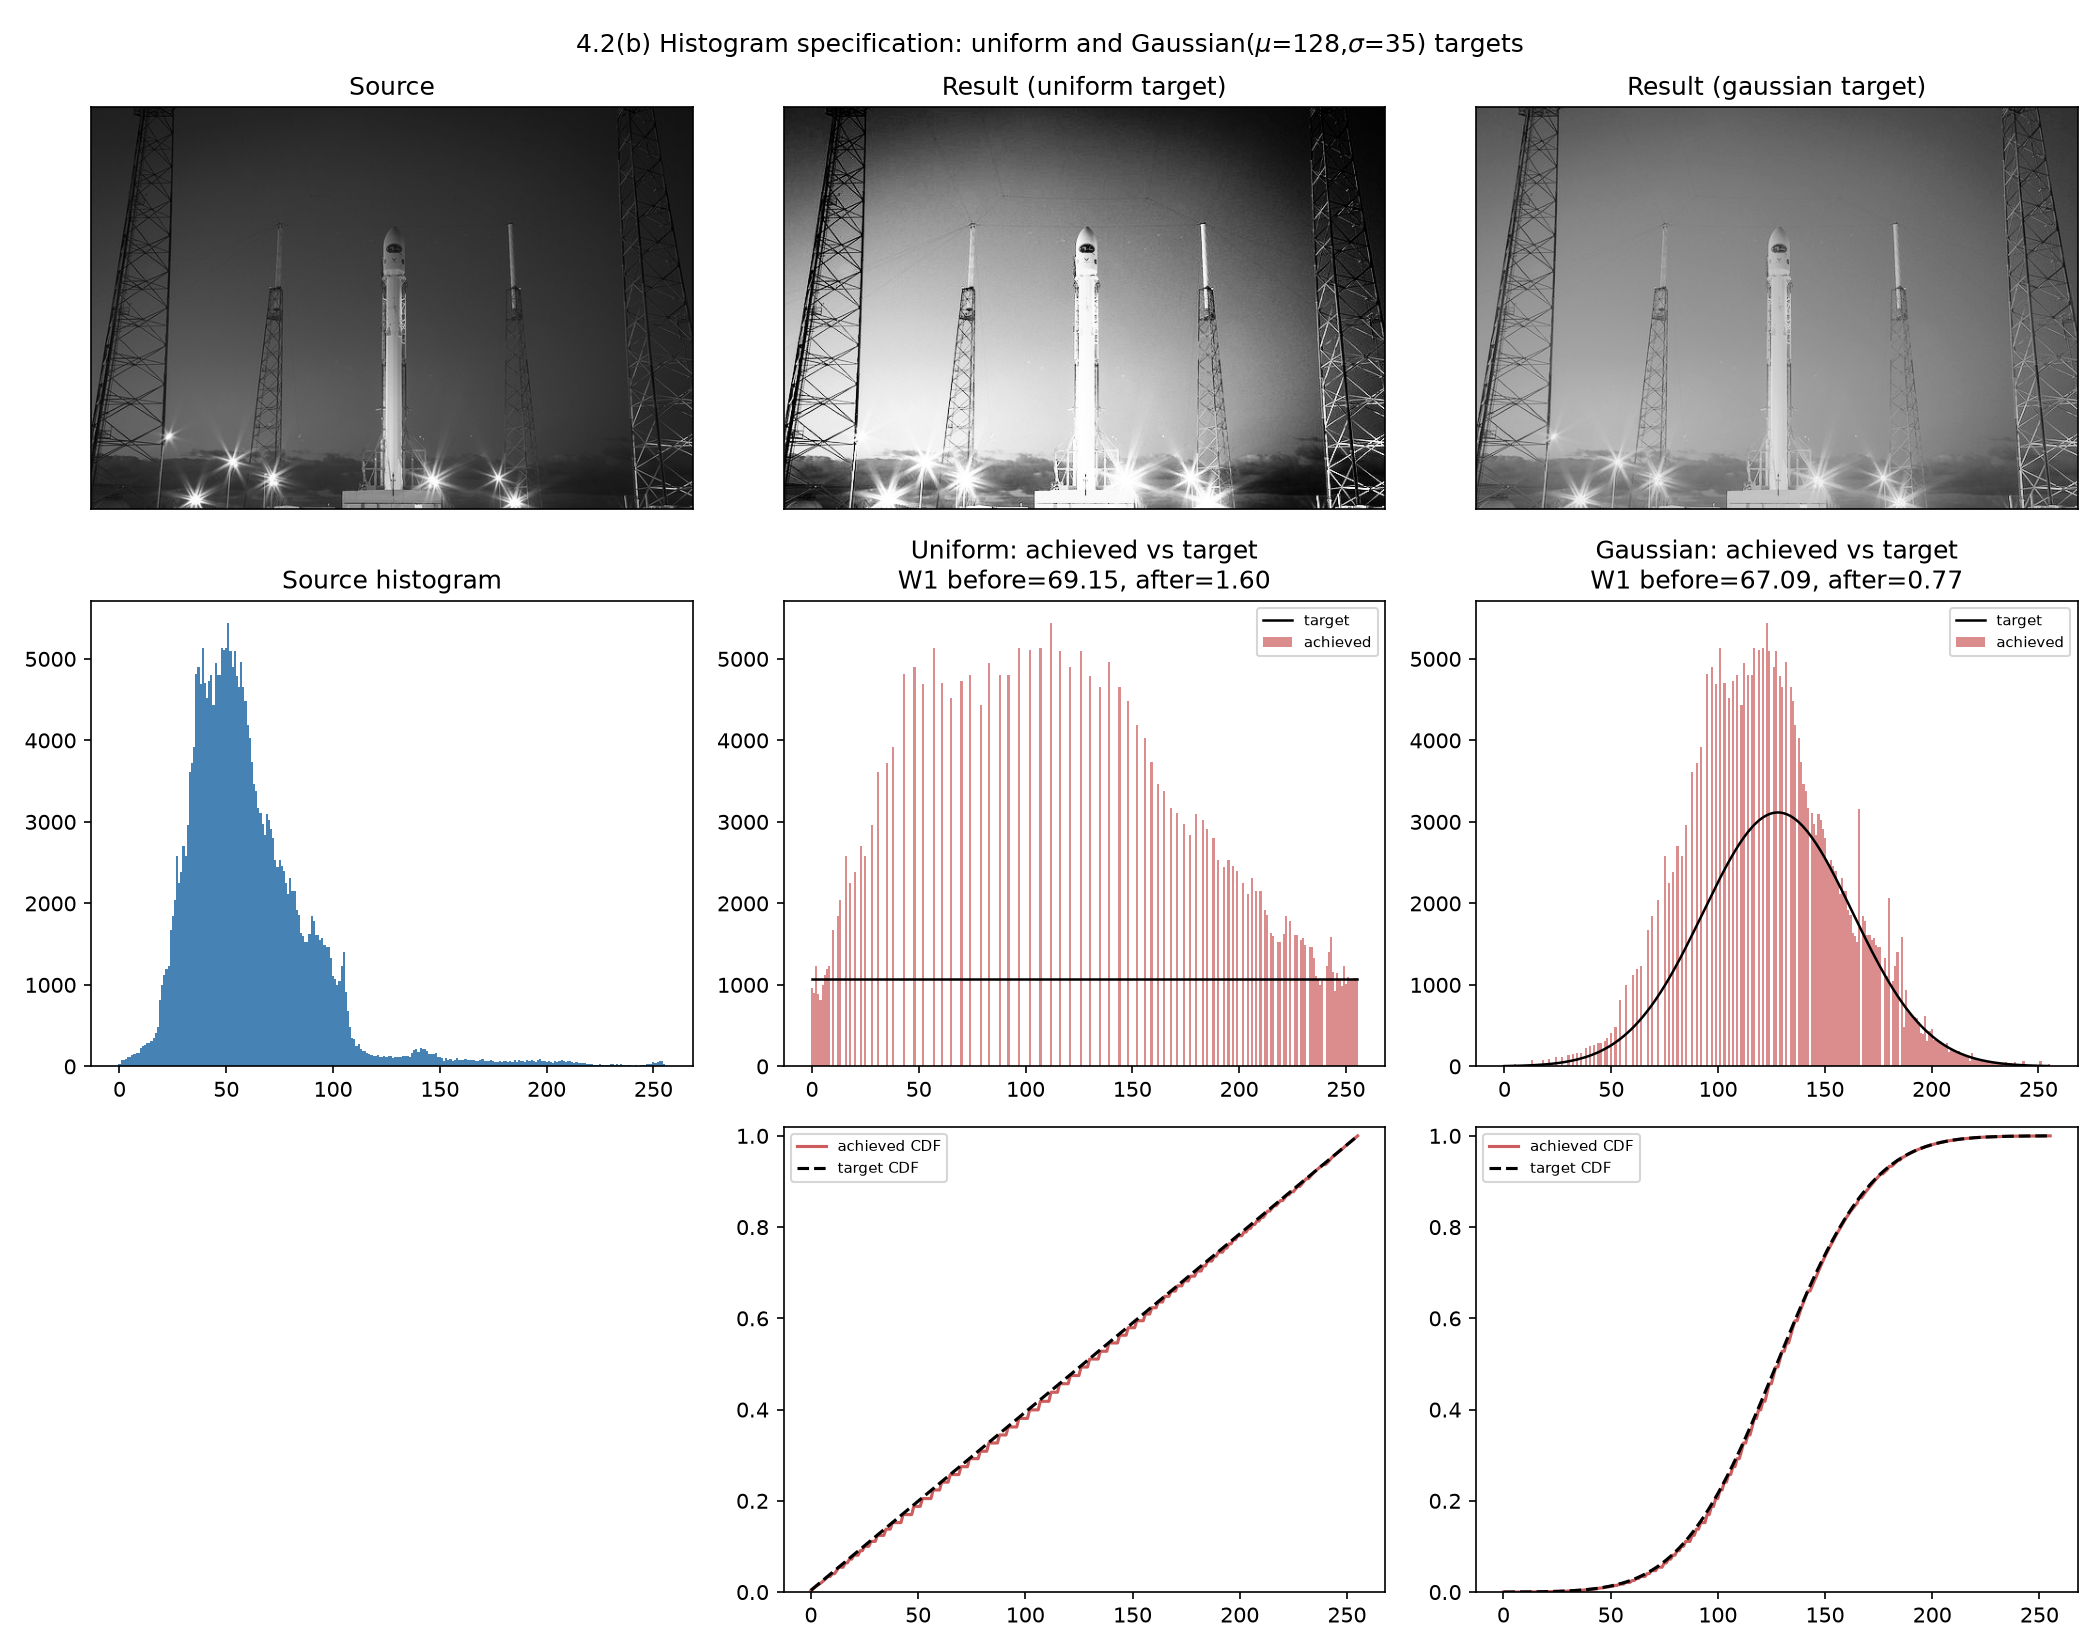
\includegraphics[width=\textwidth]{Images/p4_4_2_specification.png}
\caption{\texttt{specification/source.png} specified to a uniform target and a Gaussian
($\mu=128,\sigma=35$) target.}
\label{fig:p4_specification}
\end{figure}
Uniform specification and plain equalisation are the same operation when the target is exactly
uniform: $F_{\text{target}}(w) = w/255$, so $\text{smallest } w \text{ with } F_{\text{target}}(w)
\ge F_{\text{source}}(v)$ reduces to $w = \lceil 255 F_{\text{source}}(v)\rceil$, matching
\texttt{equalise}'s $\text{round}(255F(v))$ up to the round-vs-ceiling convention at exact
half-integer boundaries. Specification is the strictly more general operation: it supports
\emph{any} target distribution (e.g.\ the Gaussian case here), of which equalisation is the
special case where the target happens to be uniform.

\paragraph{(c) Colour.}
Colour space: RGB image converted per-pixel to HSV from scratch (max/min/delta construction);
hue $H\in[0,360)$, saturation $S\in[0,1]$. Circular hue distance: $d(h_1,h_2) = \min(|h_1-h_2|
\bmod 360,\ 360 - (|h_1-h_2| \bmod 360))$, correctly handling hue's wraparound at $0^\circ$/$360^\circ$.
Near-achromatic pixels ($S \le 0.08$) are excluded from the hue-shift statistic because hue is
numerically undefined/unstable there (a near-grey pixel's tiny RGB differences make its measured
hue essentially noise).
\begin{figure}[H]
\centering
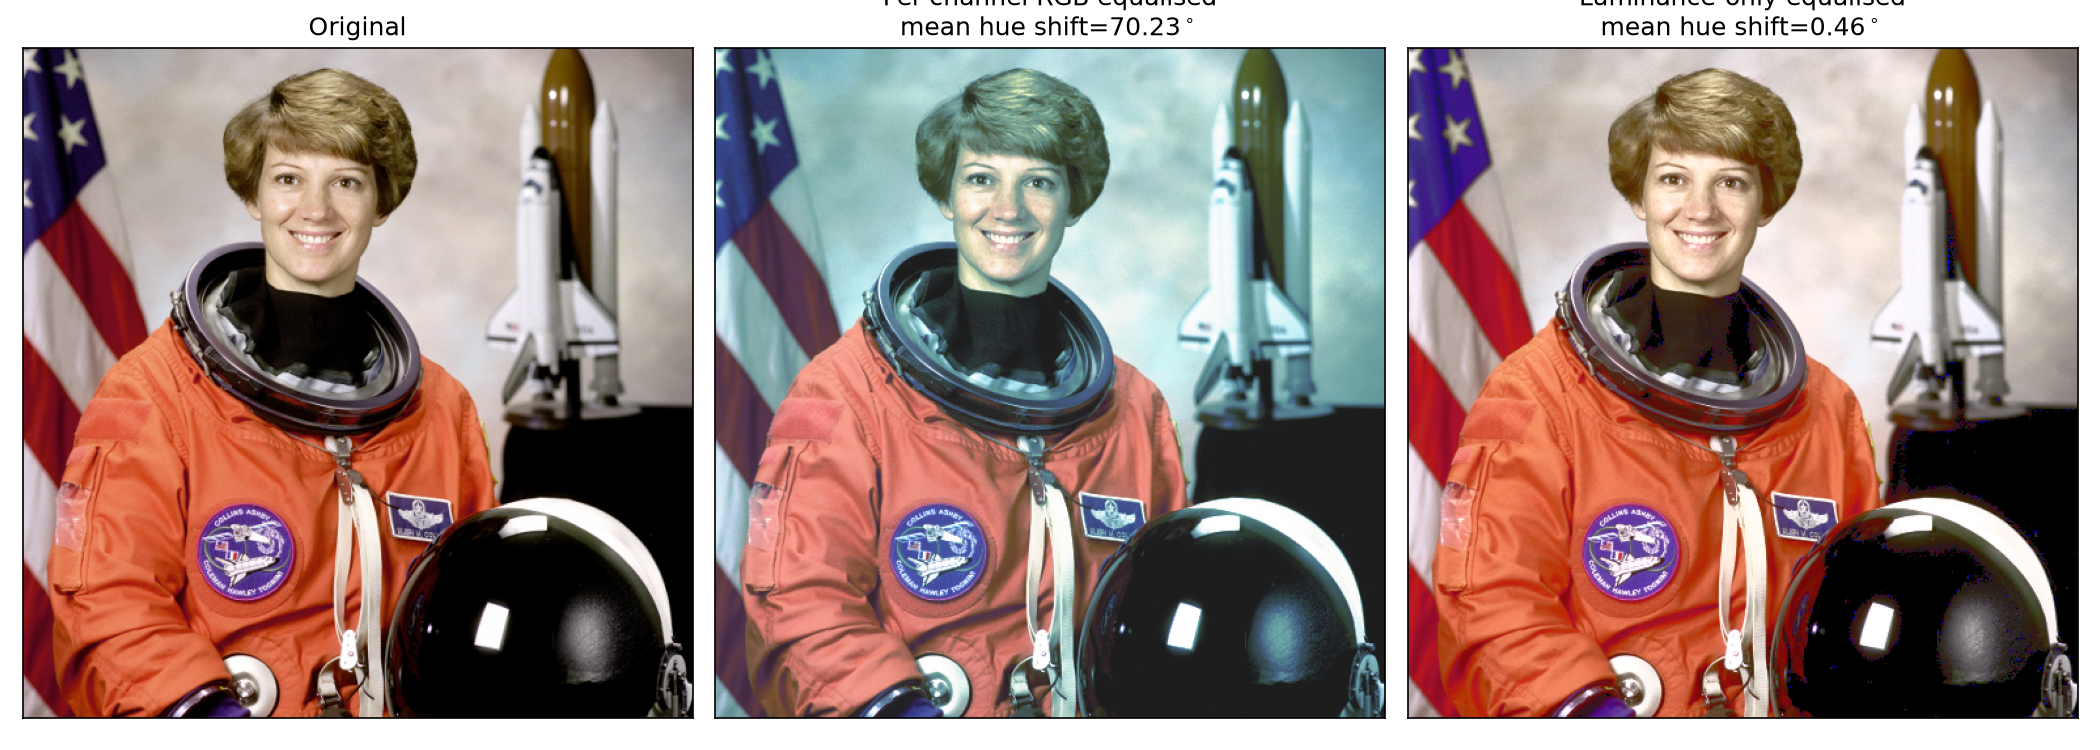
\includegraphics[width=\textwidth]{Images/p4_4_2_colour.png}
\caption{Per-channel RGB equalisation vs.\ luminance-only equalisation, \texttt{colour\_source.png}.}
\label{fig:p4_colour}
\end{figure}
Mean hue shift: per-channel equalisation $=70.23^\circ$; luminance-only equalisation
$=0.46^\circ$. Per-channel equalisation is wrong because equalisation assumes its input is a
single scalar signal whose \emph{value itself} is what should be redistributed; applying it
independently to R, G, and B computes three \emph{different} monotonic remappings (each channel
has its own histogram/CDF), which generally changes the R:G:B \emph{ratios} at a pixel --- and
hue is defined entirely by those ratios. Equalising luminance only and rescaling R,G,B by the
resulting brightness ratio changes every channel by the \emph{same} multiplicative factor at each
pixel, preserving ratios (hence hue) by construction; the $150\times$ smaller measured mean shift
confirms this is not merely a theoretical distinction.

\paragraph{Wasserstein-1 distances.}
\begin{table}[H]
\centering
% Auto-generated by run_4_2_matching.py -- do not edit by hand
\begin{tabular}{lcc}
\toprule
Target & W1 before & W1 after \\
\midrule
Image matching (source->reference) & 40.775 & 0.860 \\
Specification (uniform target) & 69.146 & 1.605 \\
Specification (gaussian target) & 67.085 & 0.767 \\
\bottomrule
\end{tabular}

\caption{W1 distance between achieved and target histogram, before (source vs.\ target) and
after (result vs.\ target), for all three matching/specification cases.}
\label{tab:p4_w1}
\end{table}
All three cases show W1 collapsing by roughly 40--90$\times$ after matching/specification,
confirming the achieved histograms closely approximate their targets --- consistent with the
visual overlays in Figures~\ref{fig:p4_matching}--\ref{fig:p4_specification} but quantified
rather than eyeballed.

\subsection{4.3 Local histogram processing (10)}
\texttt{local\_regions.png} converted once to 8-bit BT.601 luminance,
$Y=\text{round}(0.299R+0.587G+0.114B)$, used throughout this section.

\paragraph{(a) Five distinct local patches.}
\begin{figure}[H]
\centering
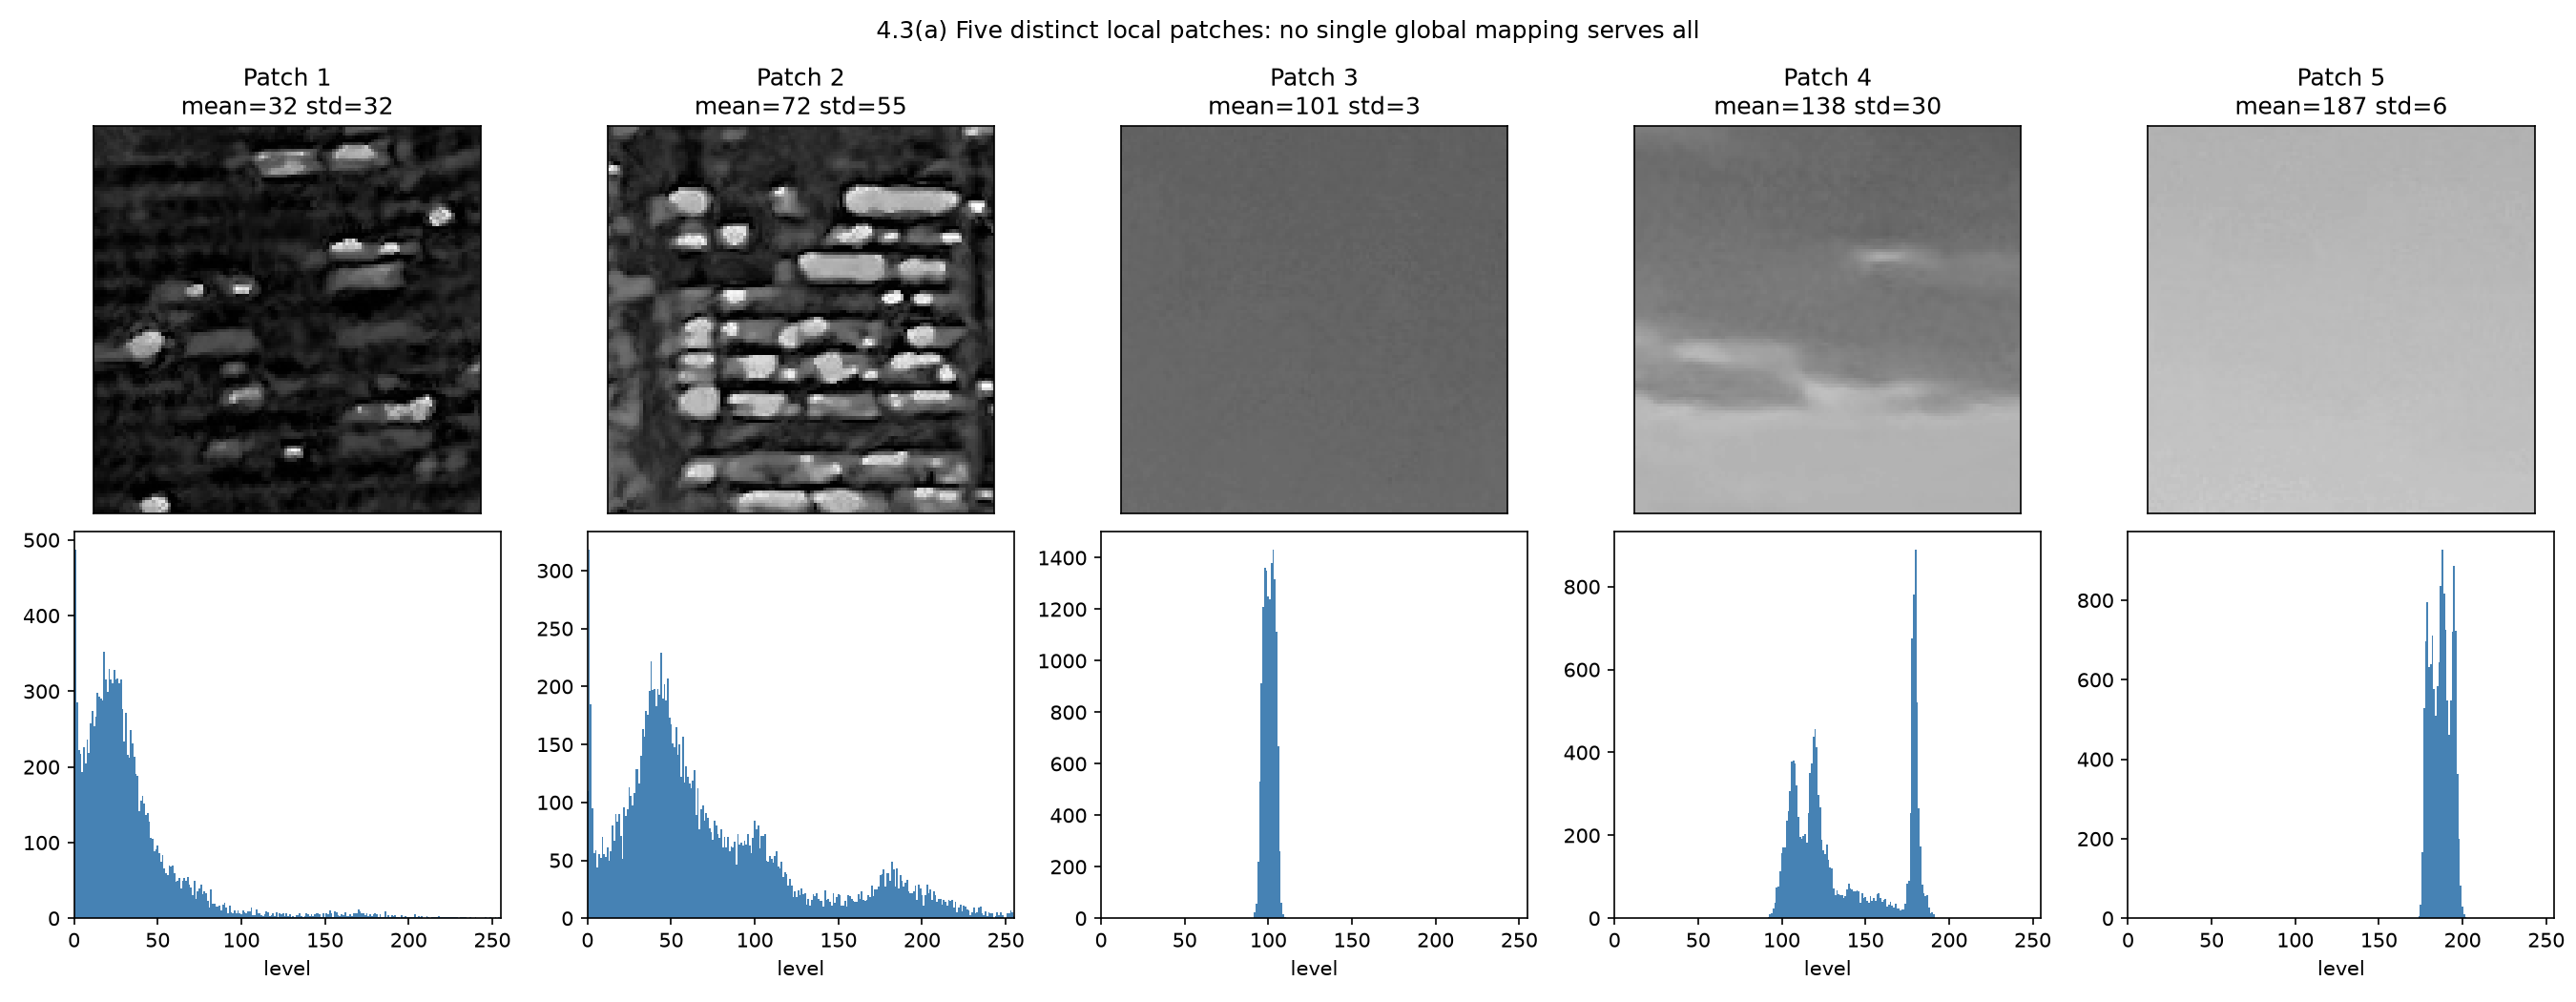
\includegraphics[width=\textwidth]{Images/p4_4_3_patches.png}
\caption{Five $120\times120$ patches spanning the image's brightness range (means
$32$--$187$), each with a markedly different local histogram.}
\label{fig:p4_patches}
\end{figure}
The five patches' histograms occupy almost disjoint intensity ranges with different shapes
(narrow/peaked vs.\ broad) --- no single global mapping $T(v)$ can simultaneously stretch the
dark patch's narrow range and preserve the already-broad bright patch's contrast, since a global
$T$ applies the same function to level $v$ regardless of which patch it came from.

\paragraph{(b) Plain tiled AHE: two failure modes.}
\begin{figure}[H]
\centering
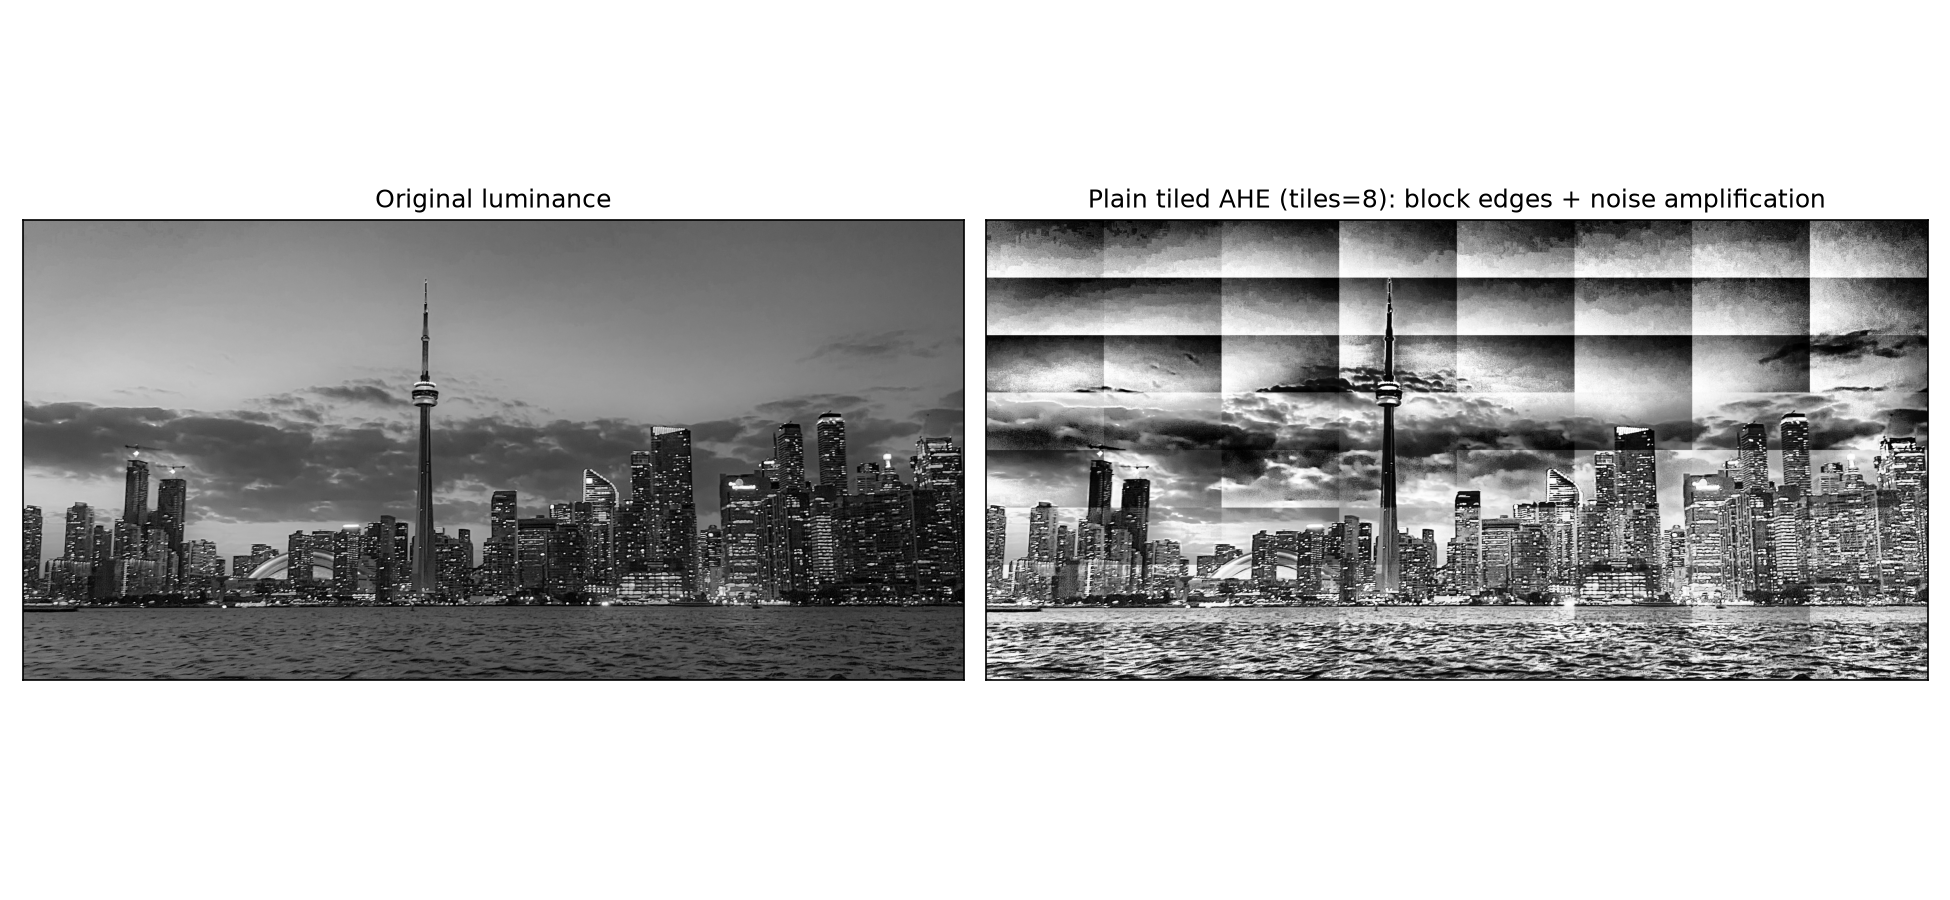
\includegraphics[width=\textwidth]{Images/p4_4_3_ahe_failure.png}
\caption{Plain tiled AHE, tiles=8: no clipping, no interpolation.}
\label{fig:p4_ahe_failure}
\end{figure}
Two failure modes are visible: (1) \textbf{hard block-boundary discontinuities} at every tile
edge --- the sky and skyline show a visible grid, because each tile is equalised by its own
completely independent LUT with no blending at the seams, so brightness can jump abruptly
crossing from one tile into its neighbour even though the underlying scene is continuous; (2)
\textbf{noise amplification in near-flat tiles} --- the sky tiles have almost no original
dynamic range (Figure~\ref{fig:p4_ahe_noise}, flattest tile std $\approx4.7$), so equalising them
independently stretches their tiny natural variation (including sensor noise/banding) across the
full 0--255 range, turning a smooth sky into visible grain.
\begin{figure}[H]
\centering
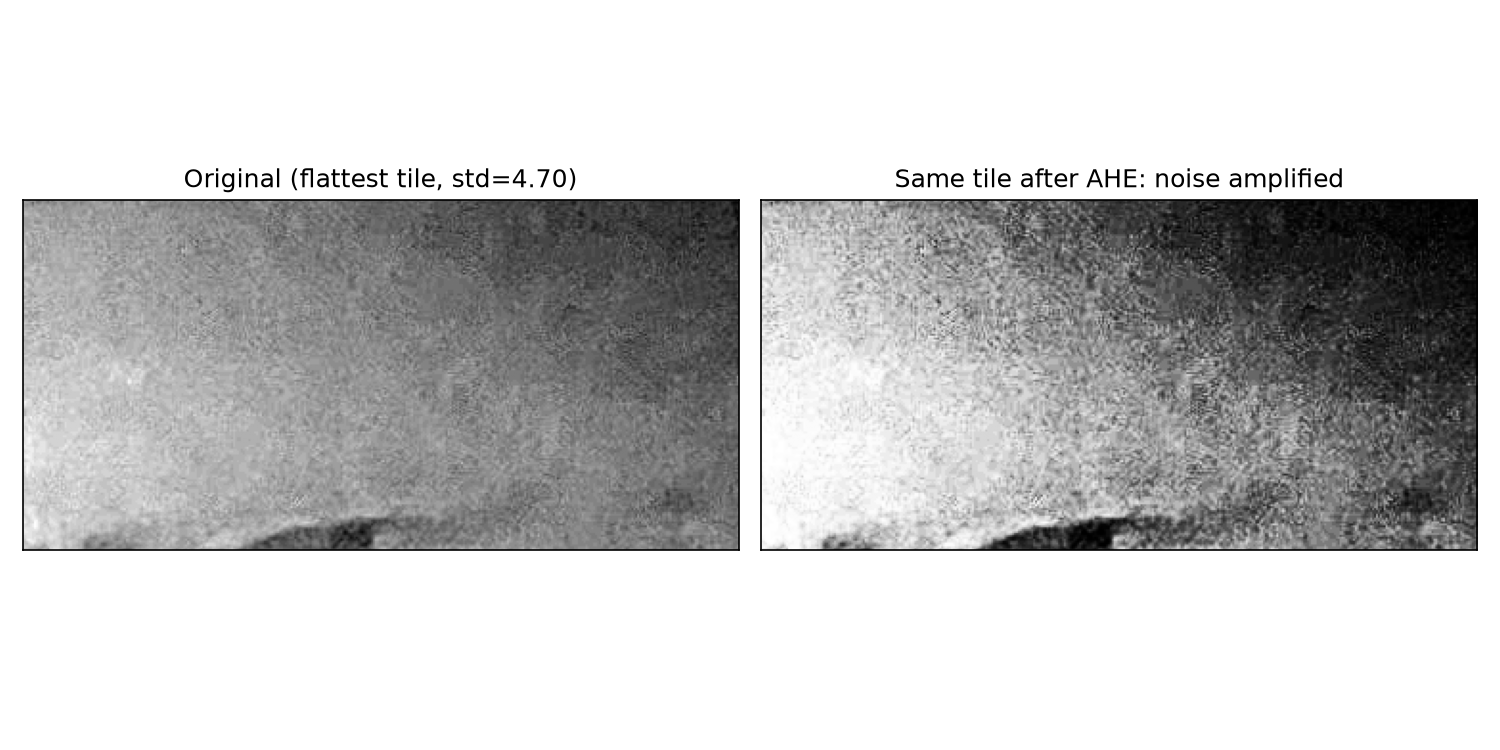
\includegraphics[width=0.7\textwidth]{Images/p4_4_3_ahe_noise_zoom.png}
\caption{Zoom on the flattest tile (std$\approx4.7$): AHE amplifies its tiny original variation
into visible noise.}
\label{fig:p4_ahe_noise}
\end{figure}

\paragraph{(c) CLAHE.}
\begin{figure}[H]
\centering
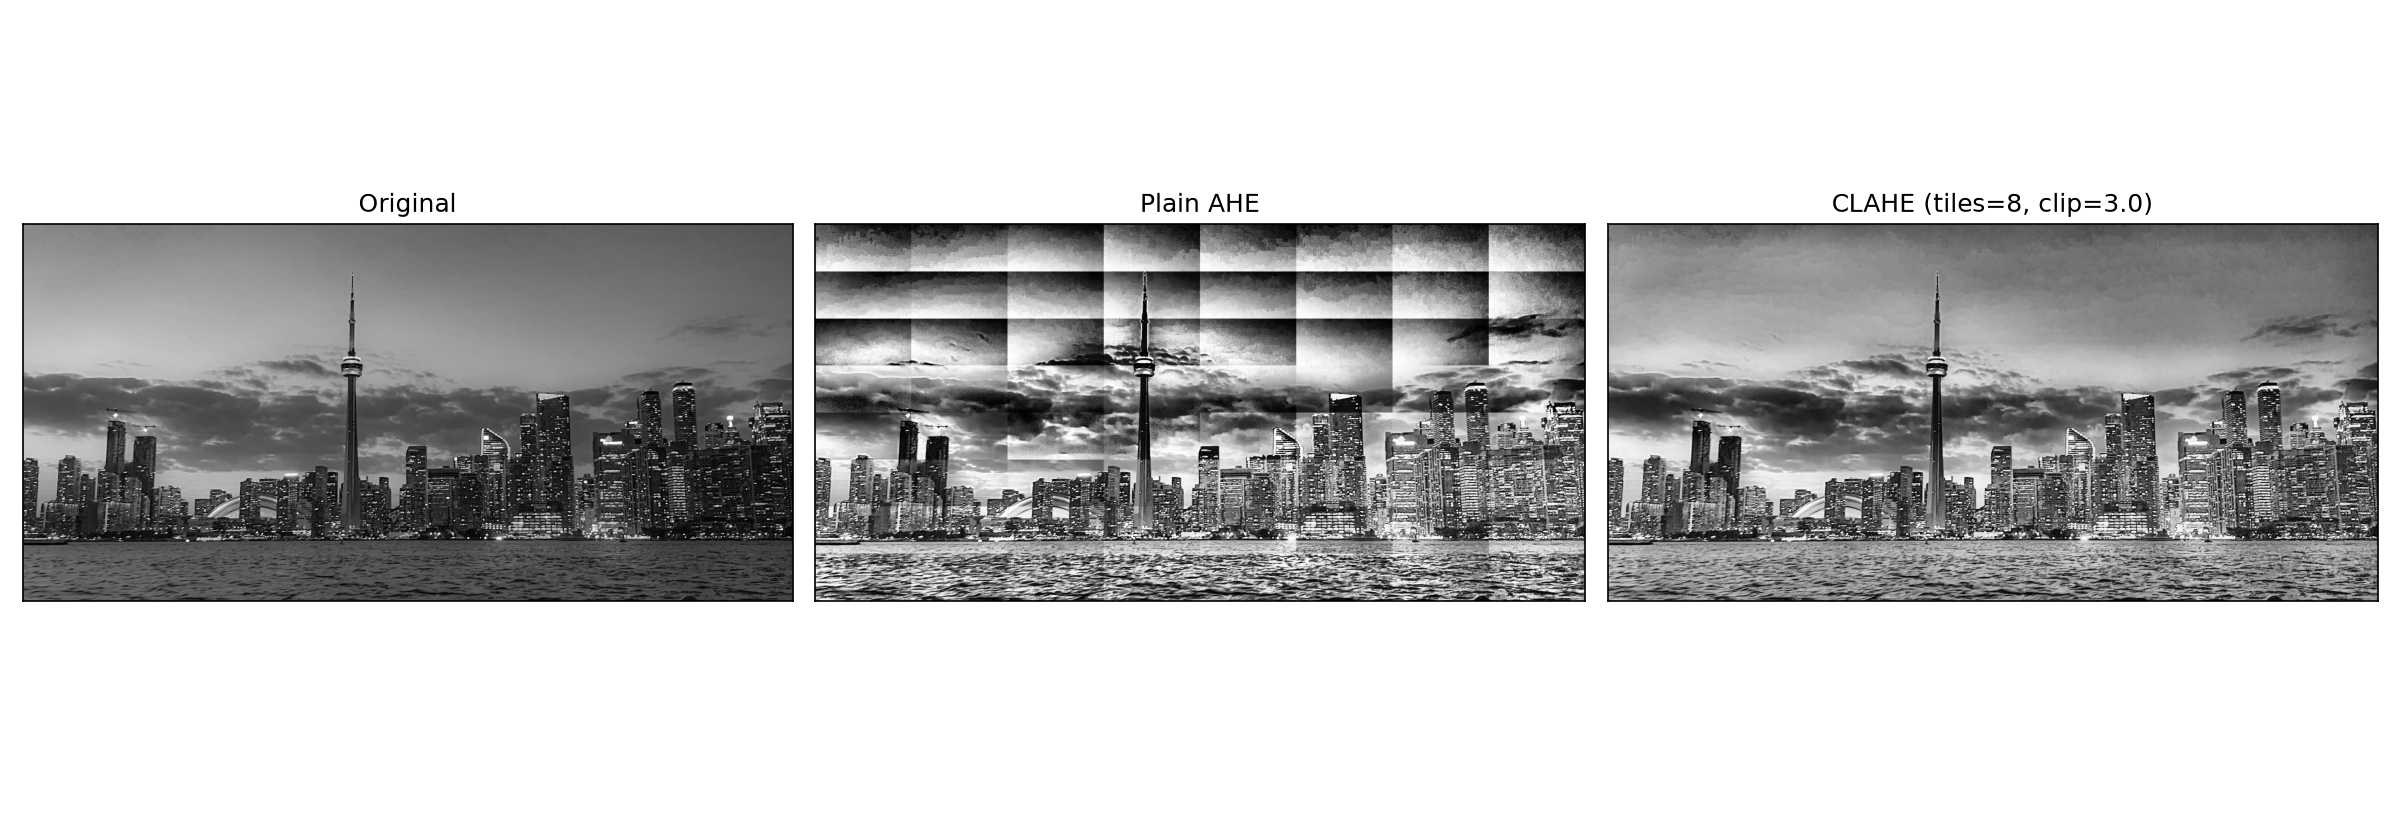
\includegraphics[width=\textwidth]{Images/p4_4_3_clahe.png}
\caption{Original, plain AHE, and CLAHE (tiles=8, clip=3.0) side by side.}
\label{fig:p4_clahe}
\end{figure}
CLAHE (clip-limited tile histograms, excess redistributed uniformly, bilinear interpolation
between the four surrounding tile-\emph{centre} LUTs at every pixel) removes both AHE failure
modes: no visible tile-boundary discontinuities (interpolation blends adjacent tiles' mappings
smoothly), and no runaway noise amplification in flat regions (the clip limit caps how much any
one bin's count -- including a flat tile's narrow spike -- can dominate its LUT's slope).

\paragraph{(d) Ablation: clip limit $\times$ tile count.}
\begin{figure}[H]
\centering
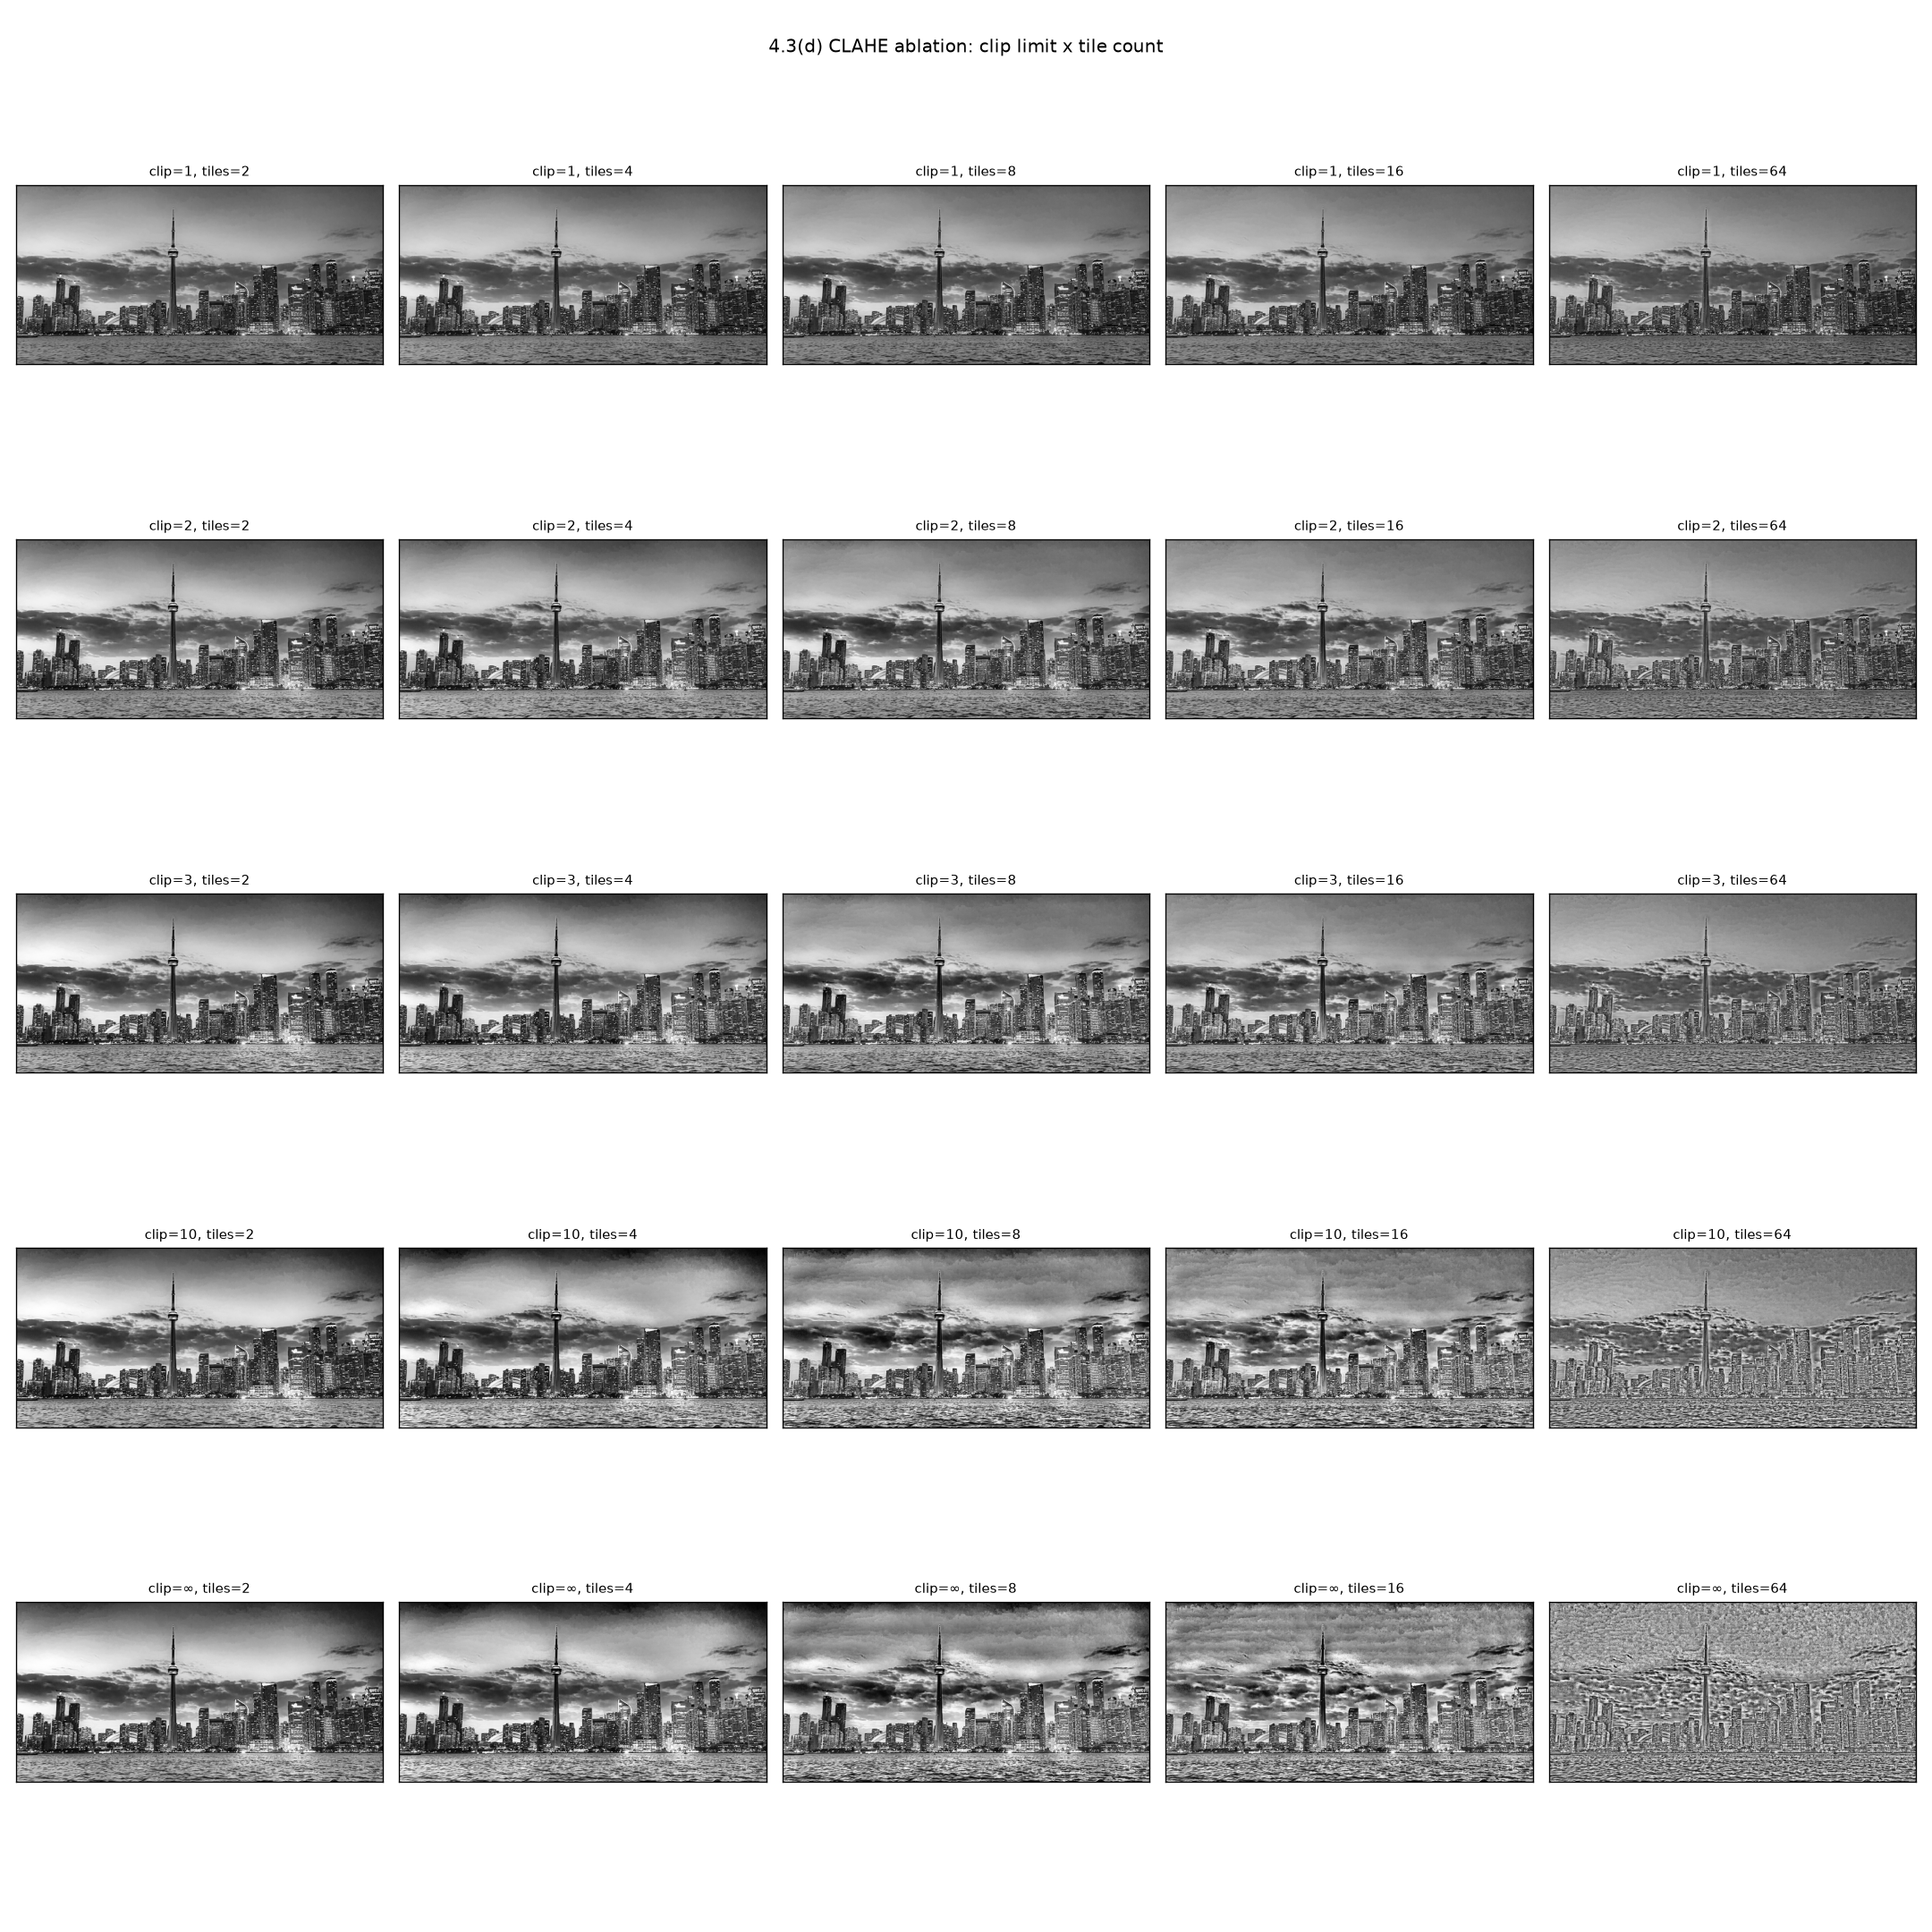
\includegraphics[width=\textwidth]{Images/p4_4_3_ablation.png}
\caption{CLAHE output over clip $\in\{1,2,3,10,\infty\}$ (rows) and tiles
$\in\{2,4,8,16,64\}$ (columns).}
\label{fig:p4_ablation}
\end{figure}
Both axes have a clear degenerate end. \textbf{Clip} $\to 1$ (top row): the clip limit is so
tight that almost every tile histogram is clipped nearly flat before it can enhance contrast at
all, and the result is close to the unmodified original --- under-enhancement. \textbf{Clip}
$\to\infty$ (bottom row): clipping is disabled, so CLAHE degenerates towards plain (interpolated)
AHE, and the noise-amplification failure mode of \S4.3(b) reappears, worst at large tile counts.
\textbf{Tiles} $\to 2$ (left column): each tile spans roughly half the image, so "local" contrast
is barely more local than a single global equalisation, and distant regions with very different
brightness are forced through the same coarse mapping. \textbf{Tiles} $\to 64$ (right column,
bottom rows especially): tiles become tiny (a few dozen pixels), each with too few pixels to
estimate a stable histogram, and combined with a loose clip limit this is the worst cell in the
grid --- visibly the noisiest, blockiest result, both failure modes compounding at once.

\paragraph{(e) Local histogram specification vs.\ CLAHE.}
\begin{figure}[H]
\centering
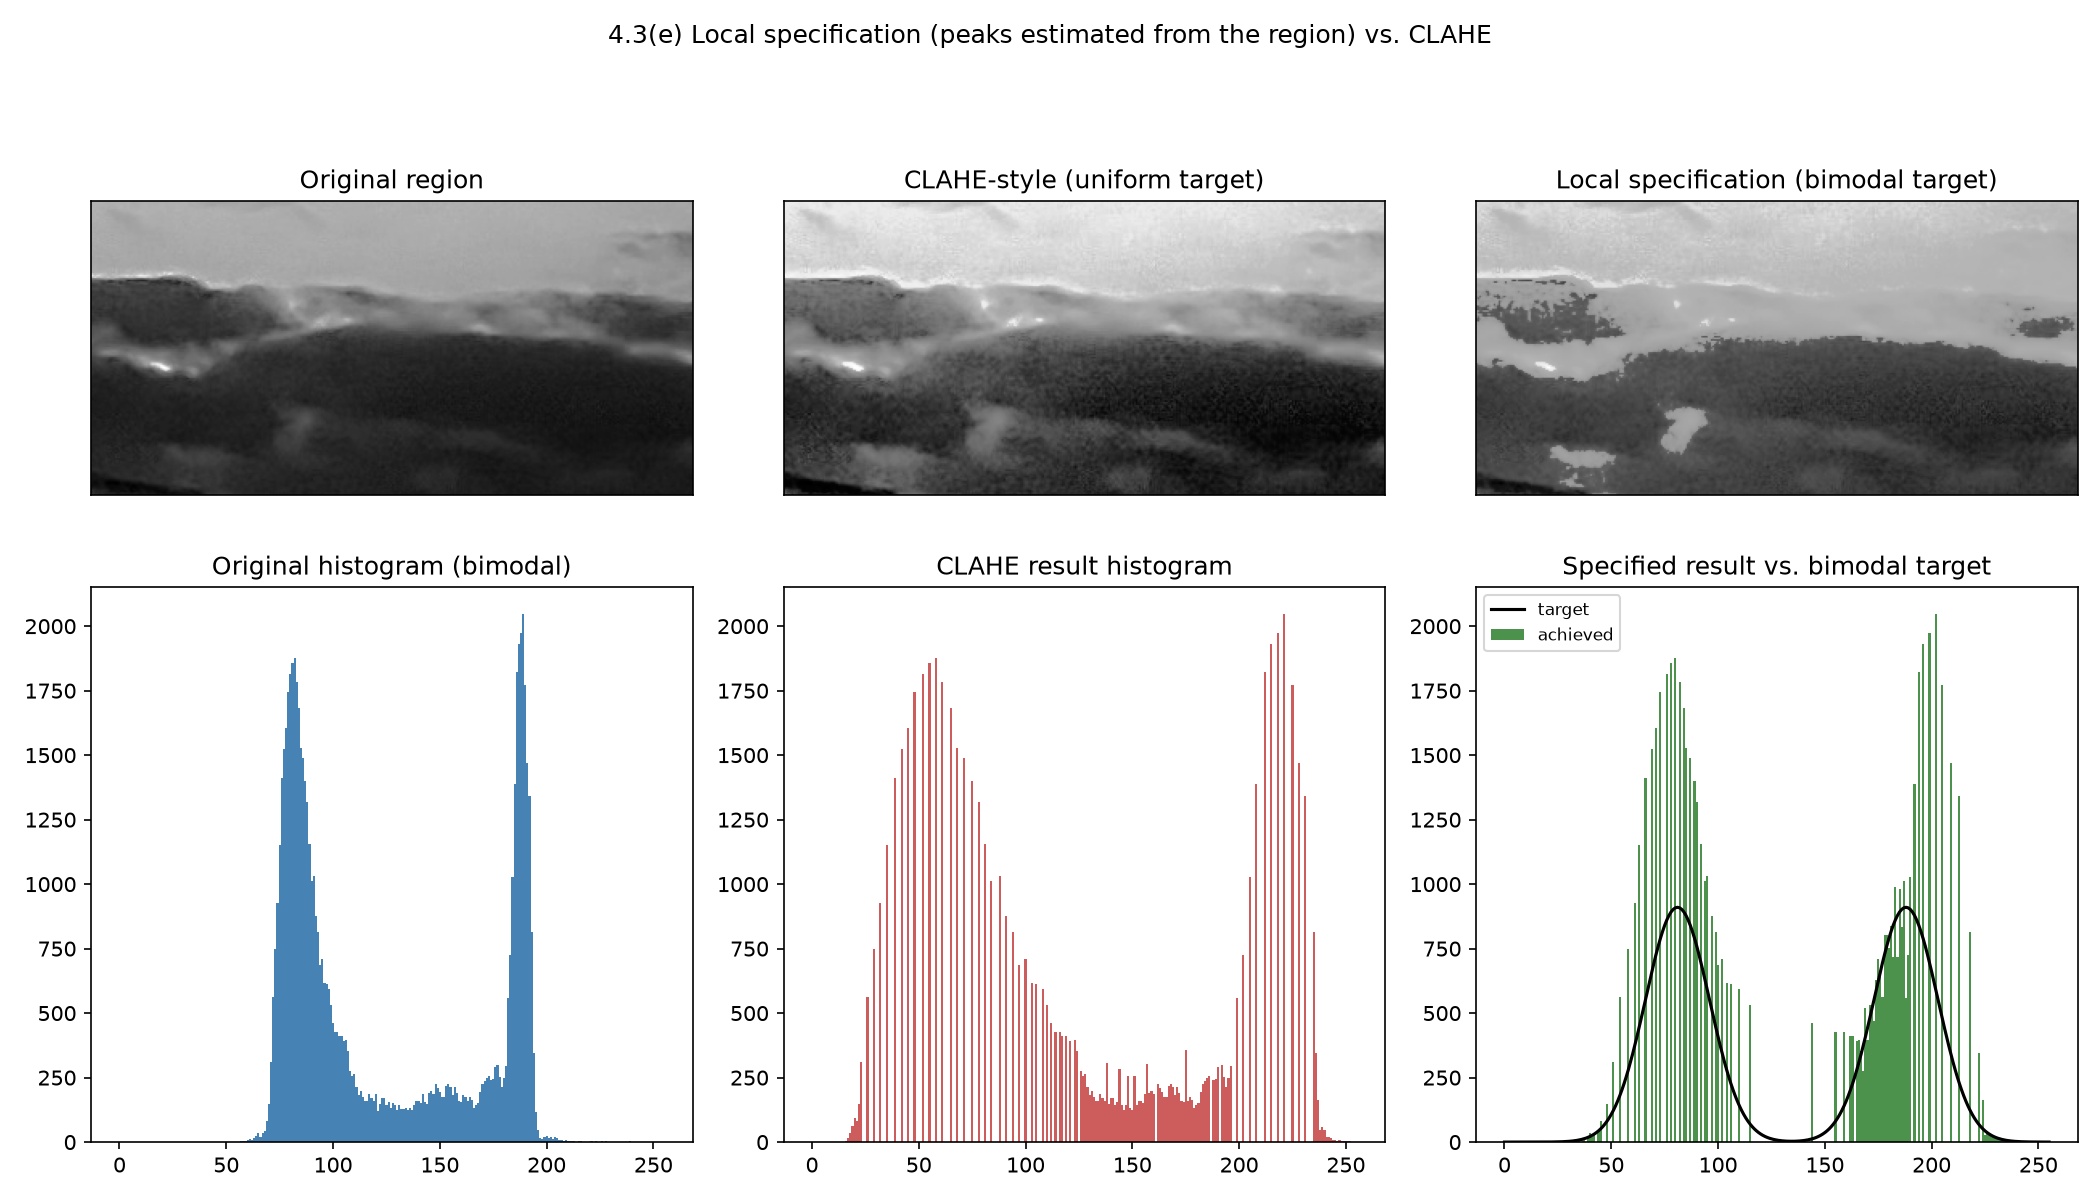
\includegraphics[width=\textwidth]{Images/p4_4_3_local_specification.png}
\caption{A region with a strongly bimodal histogram (bright sky + dark silhouette): CLAHE-style
(uniform target) vs.\ local specification to a bimodal target estimated from the region's own
two histogram peaks.}
\label{fig:p4_local_spec}
\end{figure}
On a region whose histogram is genuinely bimodal (two well-separated populous intensity bands,
e.g.\ bright sky above a dark building silhouette), a uniform target (what CLAHE effectively
pushes each tile towards) spreads pixel mass evenly across all 256 levels, which necessarily
pulls some of the two original modes together and can blur the boundary between them. Specifying
directly to a bimodal target --- two Gaussians centred on the region's own two histogram peaks
--- preserves the two-population structure explicitly rather than as a side effect of clipping.
The extra information this needs beyond CLAHE: an appropriate \emph{target shape} for the region,
here estimated from the region's own smoothed histogram peaks rather than assumed uniform ---
knowledge CLAHE does not use because it always targets (a clipped approximation of) uniform.

\subsection{4.4 Automatic correction (4)}

\paragraph{Estimator.} \texttt{auto\_correct} applies a percentile-based linear contrast stretch
to BT.601 luma: the image's own 1st and 99th luma percentiles $p_1, p_{99}$ (computed fresh from
that image, not a fixed constant) are mapped to $0$ and $255$; R, G, B are then rescaled by the
resulting per-pixel luma ratio (as in \S4.2(c)'s luminance-only operator) so hue is preserved.
Nothing is tuned per image by hand -- $p_1,p_{99}$ \emph{are} the per-image estimate the function
computes internally, satisfying "takes an image, returns an image; anything it needs it estimates
from the image." A guard falls back to a no-op when $p_{99}-p_1 < 10$ grey levels (see failure
case below).

\begin{figure}[H]
\centering
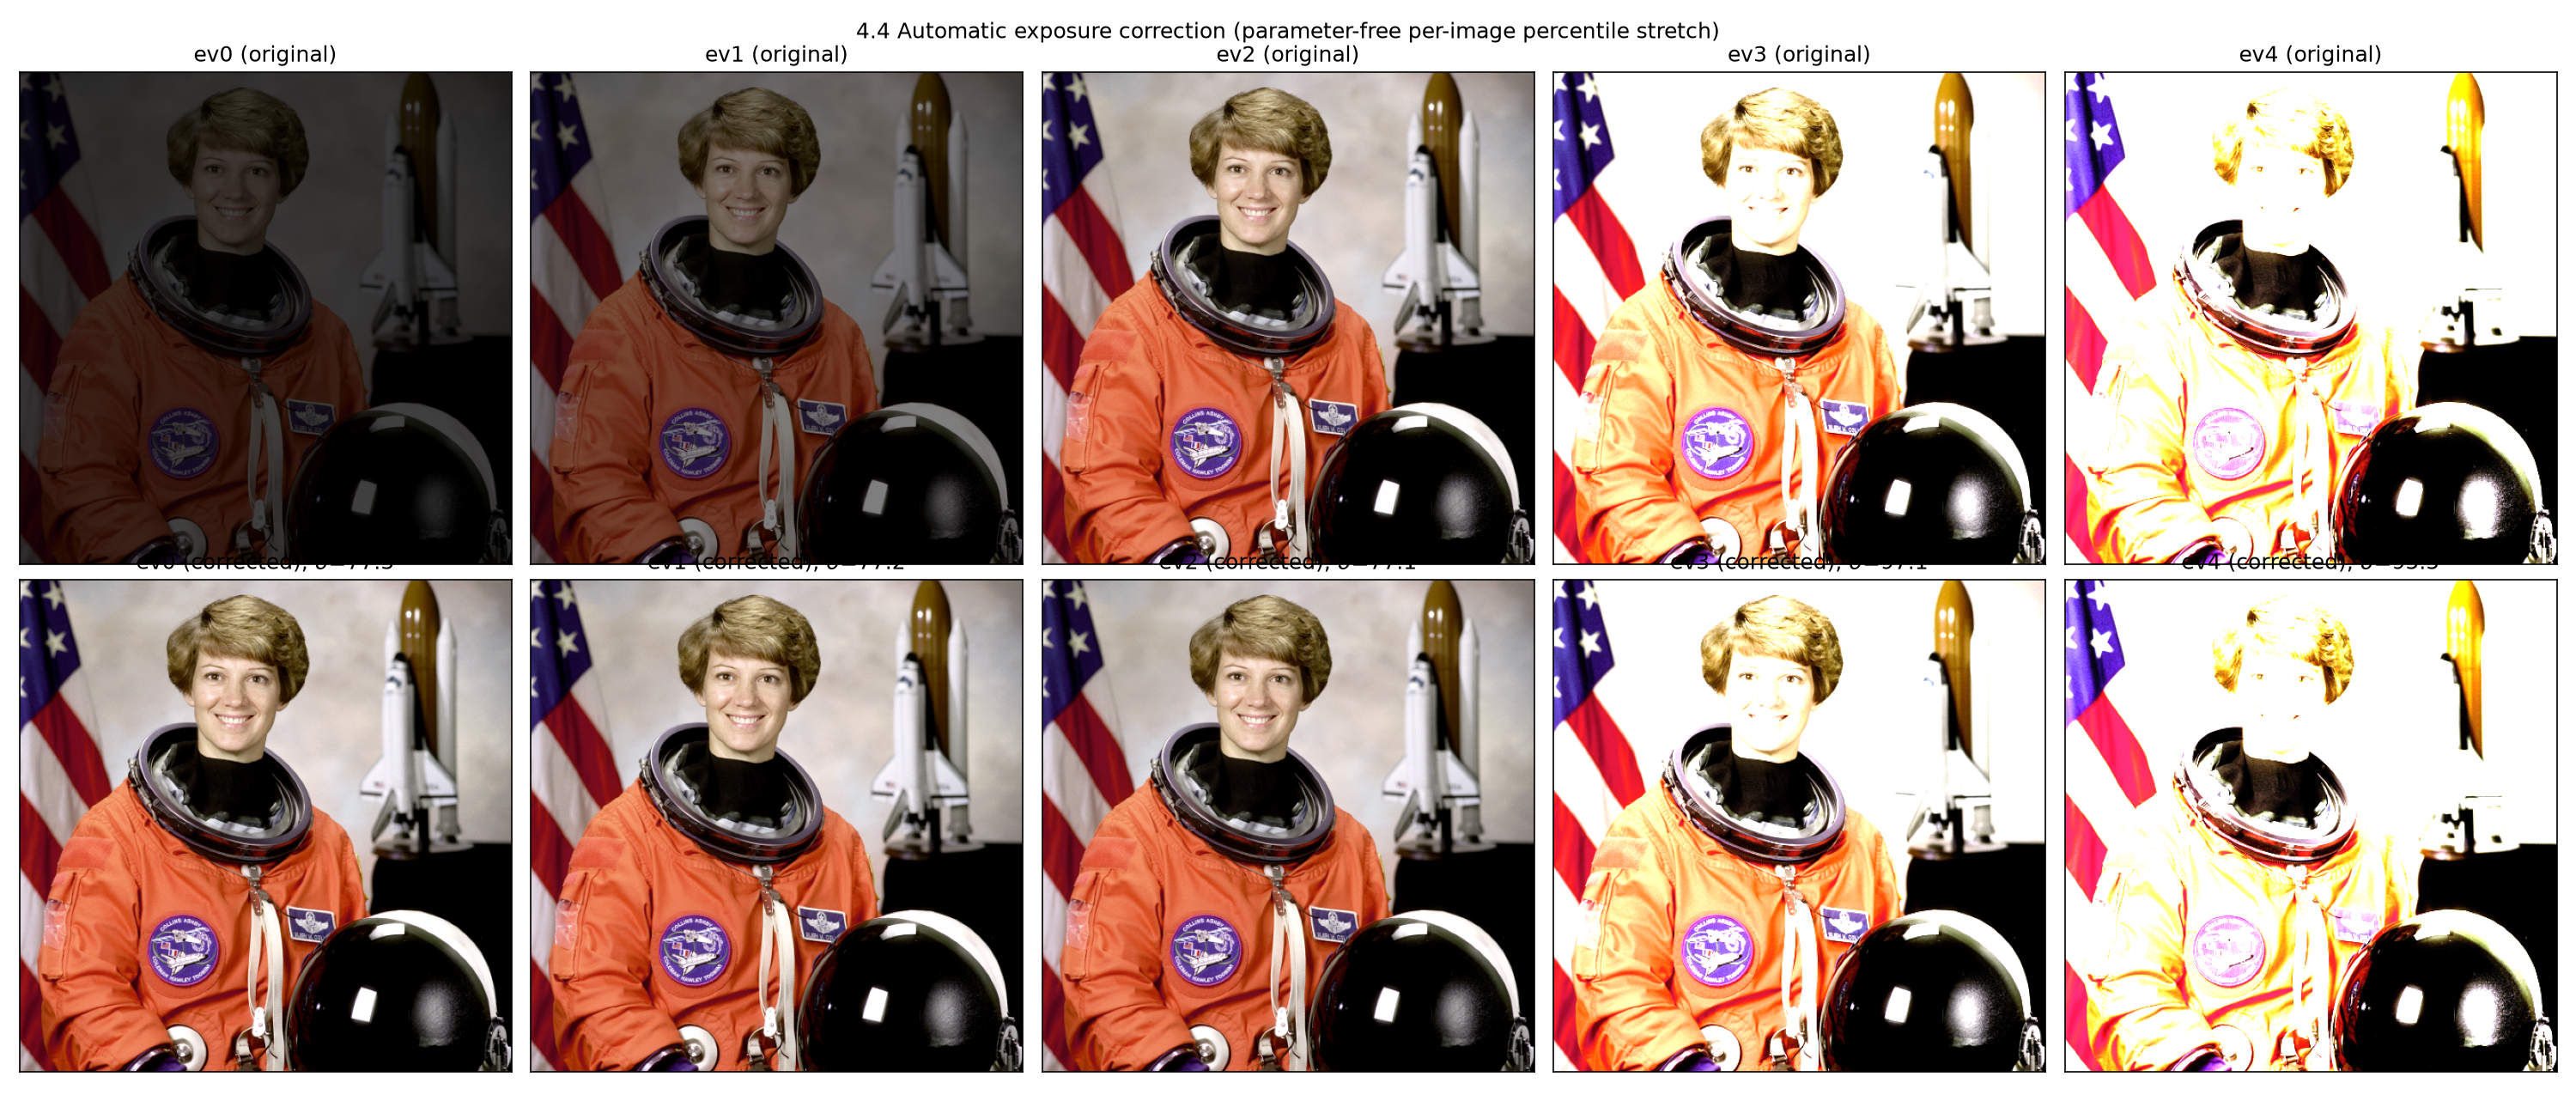
\includegraphics[width=\textwidth]{Images/p4_4_4_exposure_correction.png}
\caption{ev0--ev4 before and after \texttt{auto\_correct}.}
\label{fig:p4_exposure}
\end{figure}

\begin{table}[H]
\centering
% Auto-generated by run_4_4_auto_correct.py -- do not edit by hand
\begin{tabular}{lcc}
\toprule
Pair & W1 before & W1 after \\
\midrule
ev0--ev1 & 28.906 & 0.542 \\
ev0--ev2 & 86.632 & 0.769 \\
ev0--ev3 & 143.018 & 53.980 \\
ev0--ev4 & 165.311 & 76.273 \\
ev1--ev2 & 57.726 & 0.336 \\
ev1--ev3 & 114.112 & 53.461 \\
ev1--ev4 & 136.404 & 75.753 \\
ev2--ev3 & 56.386 & 53.247 \\
ev2--ev4 & 78.679 & 75.539 \\
ev3--ev4 & 22.293 & 22.293 \\
\midrule
Mean & 88.947 & 41.219 \\
Max & 165.311 & 76.273 \\
\bottomrule
\end{tabular}

\caption{W1 distance (normalised luma histograms) between every pair of the five exposures,
before and after correction.}
\label{tab:p4_4_4_w1}
\end{table}

Mean pairwise W1 drops from $88.9$ to $41.2$; the largest reductions are among the pairs that
\emph{can} be corrected (ev0--ev2: $86.6\to0.77$; ev1--ev2: $57.7\to0.34$; ev0--ev1:
$28.9\to0.54$) --- these three exposures' clipping is mild enough that $p_1,p_{99}$ give a
reliable stretch, and after correction they agree almost exactly.

\begin{table}[H]
\centering
% Auto-generated by run_4_4_auto_correct.py -- do not edit by hand
\begin{tabular}{lccc}
\toprule
Image & Output luma std & 1st pct & 99th pct \\
\midrule
ev0 & 77.26 & 0 & 254 \\
ev1 & 77.24 & 0 & 253 \\
ev2 & 77.12 & 0 & 254 \\
ev3 & 97.14 & 0 & 255 \\
ev4 & 95.51 & 0 & 255 \\
\bottomrule
\end{tabular}

\caption{Output luma standard deviation and 1st/99th percentile range per image, confirming
non-degenerate (non-constant) output.}
\label{tab:p4_4_4_stats}
\end{table}

Every corrected output has luma std $\ge77$ and a 1st--99th percentile range $\ge253$ --- i.e.\
none of the five collapses to a constant or near-constant image, which would trivially zero every
pairwise W1 (an invalid "solution" the handout explicitly warns against) while destroying all
image content; the corrected outputs remain full-range, detailed images.

\paragraph{Concrete failure case.} ev3 and ev4 are already badly overexposed (ev4's luma
\emph{median} is $255$, i.e.\ more than half the image is fully clipped white) and, measured,
both have $p_1=0$, $p_{99}=255$ -- their percentile spread is not small (the small-spread guard
does not fire), because enough shadow \emph{and} highlight pixels are already clipped that the
distribution spans the full range regardless of how much genuine mid-tone detail survives. The
stretch $(Y-p_1)\cdot255/(p_{99}-p_1)$ then reduces to the identity ($p_1=0,p_{99}=255$
$\Rightarrow$ no rescaling), so \texttt{auto\_correct} leaves both essentially unchanged --- which
is visible in the W1 table as ev3--ev4 being completely unchanged by correction ($22.293\to
22.293$ identically) and every pair involving ev3 or ev4 remaining at high residual W1
($53$--$76$) even after correction, versus near-zero for the three well-exposed images. The
deeper problem is structural, not a mistuned threshold: once a pixel is clipped to 0 or 255 in
the original 8-bit capture, the information needed to recover its true brightness is gone, and no
image-domain estimator --- percentile-based or otherwise --- can invert that many-to-one clip.
Because the clipped mass at both ends inflates the measured spread to look like a healthy,
full-range image, a percentile estimator cannot even reliably \emph{detect} this failure from
$p_1,p_{99}$ alone; a more robust estimator would need to look at what \emph{fraction} of pixels
sit exactly at 0 or 255, not just the percentile values, to recognise saturation directly. This is
a real limitation of purely image-domain auto-correction, not a bug specific to this estimator.

%=======================================================================
\section{Problem 5 --- Green screen compositing (15)}
%=======================================================================

\todoblock{Source qualifying footage (720p+, hair/motion-blur/translucent subject on green
backing, 48 frames) and a background plate $\geq 2.5\times$ frame width; state the clip choice
and why it qualifies.}

\subsection{5.1 Naive key (3)}
\todoblock{Threshold on green dominance in raw RGB, then key on chroma alone in YCbCr or HSV;
identify a specific failing pixel for the RGB version and explain the RGB property responsible.}

\subsection{5.2 Soft matte and spill suppression (7)}
\todoblock{(a) Chroma-distance distributions for backing / partially-transparent / foreground
pixels; state whether the three populations separate.}

\todoblock{(b) Continuous alpha from chroma distance; composite $I = \alpha F + (1-\alpha)B$;
report the fraction of pixels with fractional alpha.}

\todoblock{(c) Spill suppression scaling with $(1-\alpha)$; measure residual green excess over
fractional-alpha pixels only.}

\todoblock{(d) Compare naive vs.\ soft mattes: mean absolute difference of alpha maps and of
their gradient fields; explain the disagreement.}

\subsection{5.3 Video, efficiently (5)}
\todoblock{Vectorised compositing of 48 frames against a panning background crop, encoded to
mp4; report fps and the measured bottleneck.}

\todoblock{Temporal filtering to reduce flicker (measured in a static region or after
motion-aligning consecutive mattes); show the flicker measure drops and moving edges are not
smeared/lagged.}

\end{document}
